\PassOptionsToPackage{unicode=true}{hyperref} % options for packages loaded elsewhere
\PassOptionsToPackage{hyphens}{url}
\PassOptionsToPackage{dvipsnames,svgnames*,x11names*}{xcolor}
%
\documentclass[ignorenonframetext,]{beamer}
\usepackage{pgfpages}
\setbeamertemplate{caption}[numbered]
\setbeamertemplate{caption label separator}{: }
\setbeamercolor{caption name}{fg=normal text.fg}
\beamertemplatenavigationsymbolsempty
% Prevent slide breaks in the middle of a paragraph:
\widowpenalties 1 10000
\raggedbottom
\setbeamertemplate{part page}{
\centering
\begin{beamercolorbox}[sep=16pt,center]{part title}
  \usebeamerfont{part title}\insertpart\par
\end{beamercolorbox}
}
\setbeamertemplate{section page}{
\centering
\begin{beamercolorbox}[sep=12pt,center]{part title}
  \usebeamerfont{section title}\insertsection\par
\end{beamercolorbox}
}
\setbeamertemplate{subsection page}{
\centering
\begin{beamercolorbox}[sep=8pt,center]{part title}
  \usebeamerfont{subsection title}\insertsubsection\par
\end{beamercolorbox}
}
\AtBeginPart{
  \frame{\partpage}
}
\AtBeginSection{
  \ifbibliography
  \else
    \frame{\sectionpage}
  \fi
}
\AtBeginSubsection{
  \frame{\subsectionpage}
}
\usepackage{lmodern}
\usepackage{amssymb,amsmath}
\usepackage{ifxetex,ifluatex}
\usepackage{fixltx2e} % provides \textsubscript
\ifnum 0\ifxetex 1\fi\ifluatex 1\fi=0 % if pdftex
  \usepackage[T1]{fontenc}
  \usepackage[utf8]{inputenc}
  \usepackage{textcomp} % provides euro and other symbols
\else % if luatex or xelatex
  \usepackage{unicode-math}
  \defaultfontfeatures{Ligatures=TeX,Scale=MatchLowercase}
\fi
% use upquote if available, for straight quotes in verbatim environments
\IfFileExists{upquote.sty}{\usepackage{upquote}}{}
% use microtype if available
\IfFileExists{microtype.sty}{%
\usepackage[]{microtype}
\UseMicrotypeSet[protrusion]{basicmath} % disable protrusion for tt fonts
}{}
\IfFileExists{parskip.sty}{%
\usepackage{parskip}
}{% else
\setlength{\parindent}{0pt}
\setlength{\parskip}{6pt plus 2pt minus 1pt}
}
\usepackage{xcolor}
\usepackage{hyperref}
\hypersetup{
            pdftitle={Introduction to R Programming},
            pdfauthor={Pedro Fonseca},
            colorlinks=true,
            linkcolor=Maroon,
            filecolor=Maroon,
            citecolor=Blue,
            urlcolor=blue,
            breaklinks=true}
\urlstyle{same}  % don't use monospace font for urls
\newif\ifbibliography
\usepackage{color}
\usepackage{fancyvrb}
\newcommand{\VerbBar}{|}
\newcommand{\VERB}{\Verb[commandchars=\\\{\}]}
\DefineVerbatimEnvironment{Highlighting}{Verbatim}{commandchars=\\\{\}}
% Add ',fontsize=\small' for more characters per line
\usepackage{framed}
\definecolor{shadecolor}{RGB}{248,248,248}
\newenvironment{Shaded}{\begin{snugshade}}{\end{snugshade}}
\newcommand{\AlertTok}[1]{\textcolor[rgb]{0.94,0.16,0.16}{#1}}
\newcommand{\AnnotationTok}[1]{\textcolor[rgb]{0.56,0.35,0.01}{\textbf{\textit{#1}}}}
\newcommand{\AttributeTok}[1]{\textcolor[rgb]{0.77,0.63,0.00}{#1}}
\newcommand{\BaseNTok}[1]{\textcolor[rgb]{0.00,0.00,0.81}{#1}}
\newcommand{\BuiltInTok}[1]{#1}
\newcommand{\CharTok}[1]{\textcolor[rgb]{0.31,0.60,0.02}{#1}}
\newcommand{\CommentTok}[1]{\textcolor[rgb]{0.56,0.35,0.01}{\textit{#1}}}
\newcommand{\CommentVarTok}[1]{\textcolor[rgb]{0.56,0.35,0.01}{\textbf{\textit{#1}}}}
\newcommand{\ConstantTok}[1]{\textcolor[rgb]{0.00,0.00,0.00}{#1}}
\newcommand{\ControlFlowTok}[1]{\textcolor[rgb]{0.13,0.29,0.53}{\textbf{#1}}}
\newcommand{\DataTypeTok}[1]{\textcolor[rgb]{0.13,0.29,0.53}{#1}}
\newcommand{\DecValTok}[1]{\textcolor[rgb]{0.00,0.00,0.81}{#1}}
\newcommand{\DocumentationTok}[1]{\textcolor[rgb]{0.56,0.35,0.01}{\textbf{\textit{#1}}}}
\newcommand{\ErrorTok}[1]{\textcolor[rgb]{0.64,0.00,0.00}{\textbf{#1}}}
\newcommand{\ExtensionTok}[1]{#1}
\newcommand{\FloatTok}[1]{\textcolor[rgb]{0.00,0.00,0.81}{#1}}
\newcommand{\FunctionTok}[1]{\textcolor[rgb]{0.00,0.00,0.00}{#1}}
\newcommand{\ImportTok}[1]{#1}
\newcommand{\InformationTok}[1]{\textcolor[rgb]{0.56,0.35,0.01}{\textbf{\textit{#1}}}}
\newcommand{\KeywordTok}[1]{\textcolor[rgb]{0.13,0.29,0.53}{\textbf{#1}}}
\newcommand{\NormalTok}[1]{#1}
\newcommand{\OperatorTok}[1]{\textcolor[rgb]{0.81,0.36,0.00}{\textbf{#1}}}
\newcommand{\OtherTok}[1]{\textcolor[rgb]{0.56,0.35,0.01}{#1}}
\newcommand{\PreprocessorTok}[1]{\textcolor[rgb]{0.56,0.35,0.01}{\textit{#1}}}
\newcommand{\RegionMarkerTok}[1]{#1}
\newcommand{\SpecialCharTok}[1]{\textcolor[rgb]{0.00,0.00,0.00}{#1}}
\newcommand{\SpecialStringTok}[1]{\textcolor[rgb]{0.31,0.60,0.02}{#1}}
\newcommand{\StringTok}[1]{\textcolor[rgb]{0.31,0.60,0.02}{#1}}
\newcommand{\VariableTok}[1]{\textcolor[rgb]{0.00,0.00,0.00}{#1}}
\newcommand{\VerbatimStringTok}[1]{\textcolor[rgb]{0.31,0.60,0.02}{#1}}
\newcommand{\WarningTok}[1]{\textcolor[rgb]{0.56,0.35,0.01}{\textbf{\textit{#1}}}}
\usepackage{graphicx,grffile}
\makeatletter
\def\maxwidth{\ifdim\Gin@nat@width>\linewidth\linewidth\else\Gin@nat@width\fi}
\def\maxheight{\ifdim\Gin@nat@height>\textheight\textheight\else\Gin@nat@height\fi}
\makeatother
% Scale images if necessary, so that they will not overflow the page
% margins by default, and it is still possible to overwrite the defaults
% using explicit options in \includegraphics[width, height, ...]{}
\setkeys{Gin}{width=\maxwidth,height=\maxheight,keepaspectratio}
\setlength{\emergencystretch}{3em}  % prevent overfull lines
\providecommand{\tightlist}{%
  \setlength{\itemsep}{0pt}\setlength{\parskip}{0pt}}
\setcounter{secnumdepth}{0}

% set default figure placement to htbp
\makeatletter
\def\fps@figure{htbp}
\makeatother


\title{Introduction to R Programming}
\providecommand{\subtitle}[1]{}
\subtitle{Data Visualitazion with ggplot2}
\author{Pedro Fonseca}
\date{20 Abril 2020}

\begin{document}
\frame{\titlepage}

\begin{frame}

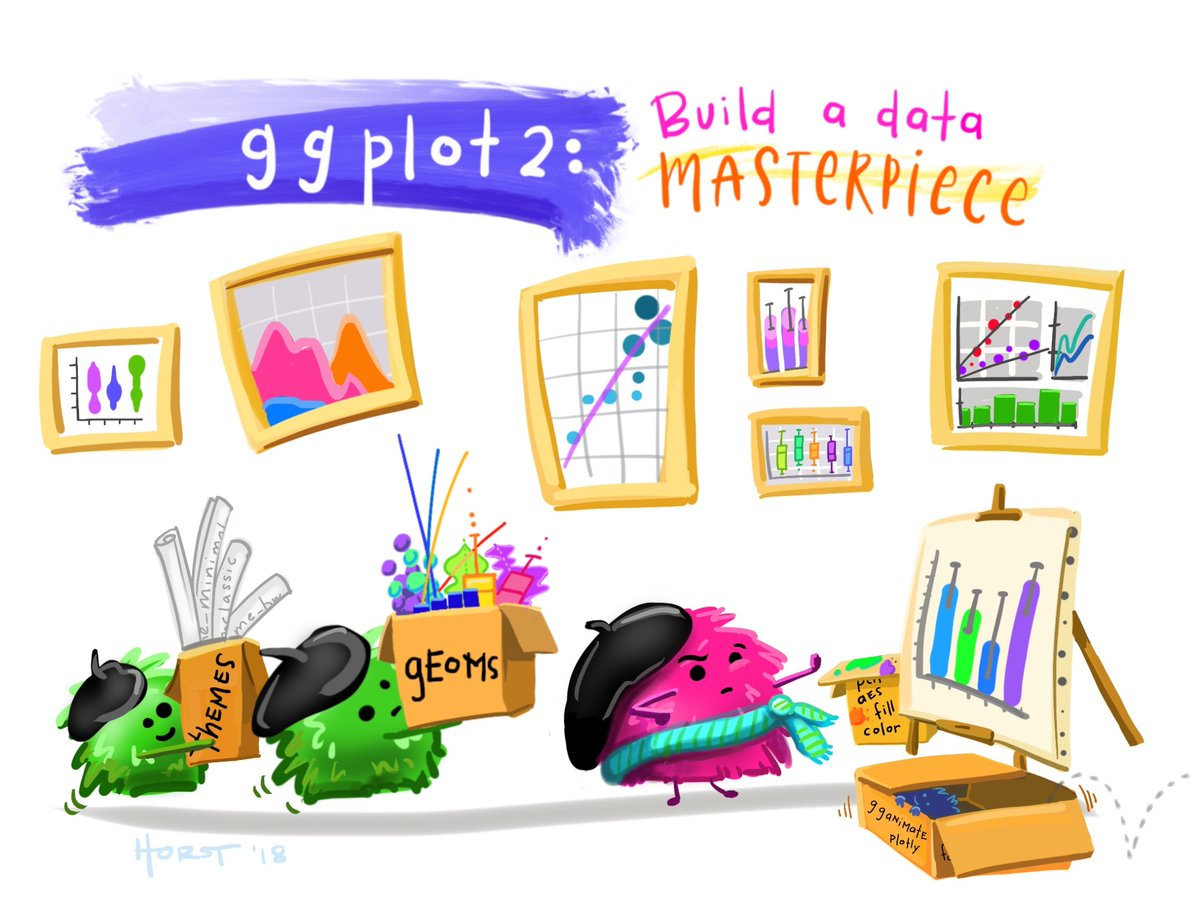
\includegraphics{figures/pic.png}

\end{frame}

\begin{frame}{Introduction}
\protect\hypertarget{introduction}{}

\begin{itemize}
\item
  In lecture you will learn how to visualise data with the ggplot2
  package.
\item
  ggplot2 is one of the most elegant and versatile systems for making
  graphs.
\item
  ggplot2 implements the grammar of graphics (Wickham 2010), a coherent
  system for describing and building graphs.
\end{itemize}

\end{frame}

\begin{frame}[fragile]{Preliminars}
\protect\hypertarget{preliminars}{}

\begin{Shaded}
\begin{Highlighting}[]
\KeywordTok{library}\NormalTok{(ggplot2)}
\end{Highlighting}
\end{Shaded}

\begin{itemize}
\tightlist
\item
  To access the datasets, help pages, and functions that we will use,
  load the ggplot2 package.
\end{itemize}

\end{frame}

\begin{frame}[fragile]{The \texttt{mpg} dataset}
\protect\hypertarget{the-mpg-dataset}{}

The \texttt{mpg} dataset contains information about 38 models of cars.
Among the variables in mpg are:

\begin{itemize}
\item
  \texttt{displ}: engine size, in litres
\item
  \texttt{cyl}: number of cylinders
\item
  \texttt{cty}: city miles per gallon
\item
  \texttt{hwy}: fuel efficiency on the highway, in miles per gallon
  (mpg).
\item
  \texttt{class}: type of car
\end{itemize}

\begin{Shaded}
\begin{Highlighting}[]
\KeywordTok{View}\NormalTok{(mpg)}
\end{Highlighting}
\end{Shaded}

For additional information see \texttt{?mpg}.

\end{frame}

\begin{frame}[fragile]{My first \texttt{ggplot()}}
\protect\hypertarget{my-first-ggplot}{}

Let's build a graph to answer the following questions:

\begin{itemize}
\item
  Do cars with big engines use more fuel than cars with small engines?
\item
  What does the relationship between engine size and fuel efficiency
  look like? Is it positive? Negative? Linear? Nonlinear?
\end{itemize}

We start by plotting engine size (\texttt{displ}) versus fuel efficiency
(\texttt{hwy}).

\end{frame}

\begin{frame}[fragile]{My first \texttt{ggplot()}}
\protect\hypertarget{my-first-ggplot-1}{}

\begin{Shaded}
\begin{Highlighting}[]
\KeywordTok{ggplot}\NormalTok{(}\DataTypeTok{data =}\NormalTok{ mpg) }\OperatorTok{+}
\StringTok{  }\KeywordTok{geom_point}\NormalTok{(}\DataTypeTok{mapping =} \KeywordTok{aes}\NormalTok{(}\DataTypeTok{x =}\NormalTok{ displ, }\DataTypeTok{y =}\NormalTok{ hwy))}
\end{Highlighting}
\end{Shaded}

\begin{center}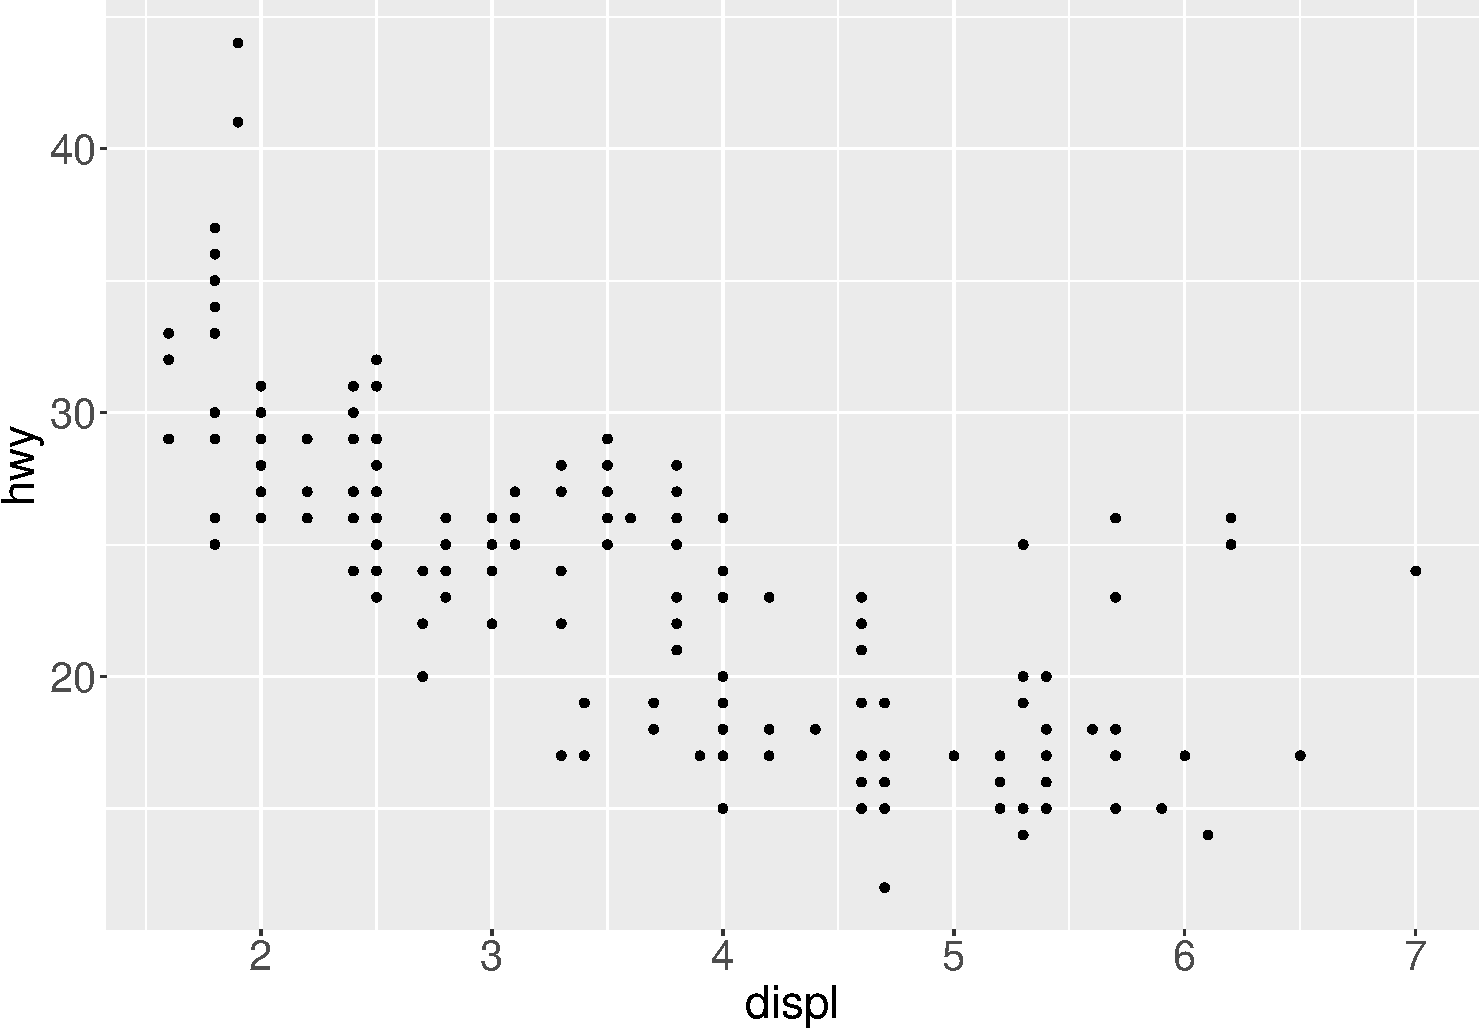
\includegraphics[height=150px]{data-visualization_files/figure-beamer/unnamed-chunk-3-1} \end{center}

\end{frame}

\begin{frame}{My first \texttt{ggplot()}}
\protect\hypertarget{my-first-ggplot-2}{}

\begin{itemize}
\item
  The plot shows a negative relationship between engine size and fuel
  efficiency.
\item
  In other words: on average, cars with big engines use more fuel.
\end{itemize}

\end{frame}

\begin{frame}[fragile]{A simple \texttt{ggplot()} template}
\protect\hypertarget{a-simple-ggplot-template}{}

\begin{Shaded}
\begin{Highlighting}[]
\KeywordTok{ggplot}\NormalTok{(}\DataTypeTok{data =} \OperatorTok{<}\NormalTok{DATA}\OperatorTok{>}\NormalTok{) }\OperatorTok{+}\StringTok{ }
\StringTok{  }\ErrorTok{<}\NormalTok{GEOM_FUNCTION}\OperatorTok{>}\NormalTok{(}\DataTypeTok{mapping =} \KeywordTok{aes}\NormalTok{(}\OperatorTok{<}\NormalTok{MAPPINGS}\OperatorTok{>}\NormalTok{))}
\end{Highlighting}
\end{Shaded}

\begin{itemize}
\item
  The first argument of \texttt{ggplot()} is a dataset
\item
  We complete the graph by adding layers to \texttt{ggplot()}
\item
  \texttt{geom\_point()} adds a layer of points, creating scatterplot.
\item
  ggplot2 has many geom functions that each add a different type of
  layer to a plot.
\end{itemize}

\end{frame}

\begin{frame}[fragile]{A simple \texttt{ggplot()} template}
\protect\hypertarget{a-simple-ggplot-template-1}{}

\begin{itemize}
\item
  Each geom function takes a \texttt{mapping} argument.
\item
  The \texttt{mapping} argument is always paired with \texttt{aes()}.
\item
  The \texttt{x} and \texttt{y} arguments of \texttt{aes()} specify
  which variables to map to the \texttt{x} and \texttt{y} axes.
\end{itemize}

\end{frame}

\begin{frame}{Geometrical objects}
\protect\hypertarget{geometrical-objects}{}

\begin{itemize}
\item
  A \textbf{geom} is the geometrical object that a plot uses to
  represent data (e.g.~points, bars, lines\ldots{}).
\item
  People often describe plots by the type of \textbf{geom} that it uses:

  \begin{itemize}
  \tightlist
  \item
    Bar charts use \textbf{bar} geoms
  \item
    Line charts use \textbf{line} geoms
  \item
    Boxplots use \textbf{boxplot} geom
  \item
    \ldots{}
  \end{itemize}
\item
  Scatterplots break the trend: they use the \textbf{point} geom.
\item
  In ggplot2, we add geoms to a plot with \textbf{geom functions}.
\end{itemize}

\end{frame}

\begin{frame}[fragile]{Geometrical objects}
\protect\hypertarget{geometrical-objects-1}{}

Compare the next two plots. How are they similar?

\begin{Shaded}
\begin{Highlighting}[]
\KeywordTok{ggplot}\NormalTok{(}\DataTypeTok{data =}\NormalTok{ mpg) }\OperatorTok{+}\StringTok{ }
\StringTok{  }\KeywordTok{geom_point}\NormalTok{(}\DataTypeTok{mapping =} \KeywordTok{aes}\NormalTok{(}\DataTypeTok{x =}\NormalTok{ displ, }\DataTypeTok{y =}\NormalTok{ hwy))}

\KeywordTok{ggplot}\NormalTok{(}\DataTypeTok{data =}\NormalTok{ mpg) }\OperatorTok{+}\StringTok{ }
\StringTok{  }\KeywordTok{geom_smooth}\NormalTok{(}\DataTypeTok{mapping =} \KeywordTok{aes}\NormalTok{(}\DataTypeTok{x =}\NormalTok{ displ, }\DataTypeTok{y =}\NormalTok{ hwy))}
\end{Highlighting}
\end{Shaded}

\end{frame}

\begin{frame}{Geometrical objects}
\protect\hypertarget{geometrical-objects-2}{}

\begin{center}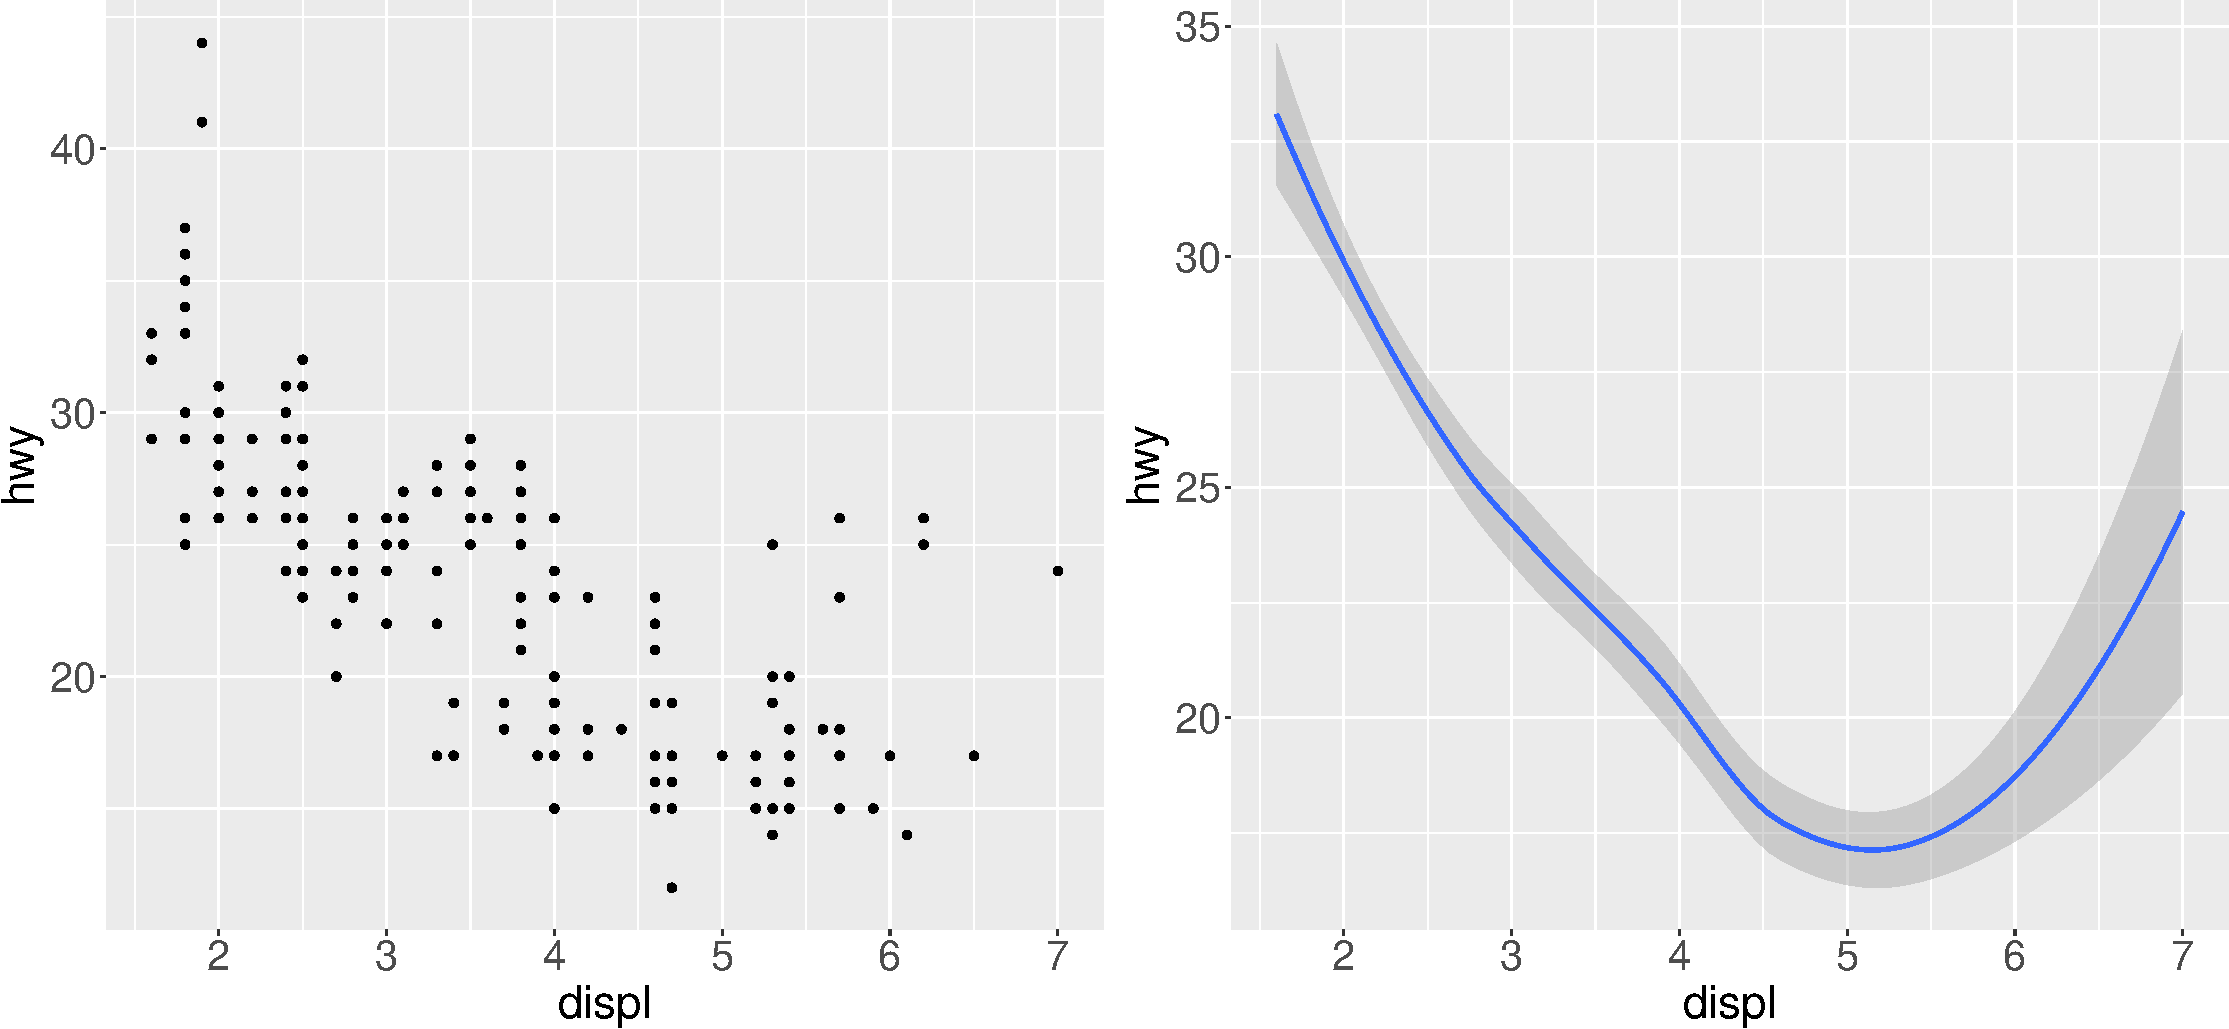
\includegraphics[height=150px]{data-visualization_files/figure-beamer/unnamed-chunk-6-1} \end{center}

\end{frame}

\begin{frame}[fragile]{Geometrical objects}
\protect\hypertarget{geometrical-objects-3}{}

Both plots:

\begin{itemize}
\item
  use the same data
\item
  have the same \texttt{x} variable
\item
  have the same \texttt{y} variable
\end{itemize}

But they are not identical:

\begin{itemize}
\item
  Each plot uses a different \textbf{geom}.
\item
  The plot on the left uses the \textbf{point} geom.
\item
  The plot on the right uses the \textbf{smooth} geom, a smooth line
  fitted to the data.
\end{itemize}

\end{frame}

\begin{frame}{The ggplot2 cheatsheet}
\protect\hypertarget{the-ggplot2-cheatsheet}{}

\begin{itemize}
\tightlist
\item
  ggplot2 provides over 40 geoms
\item
  The best way to get a comprehensive overview is the
  \href{https://rstudio.com/wp-content/uploads/2016/11/ggplot2-cheatsheet-2.1.pdf}{ggplot2
  cheatsheet}.
\end{itemize}

\end{frame}

\begin{frame}[fragile]{Aesthetics}
\protect\hypertarget{aesthetics}{}

\begin{itemize}
\item
  \textbf{Aesthetics} are visual properties of the \textbf{geoms}.
\item
  \textbf{Aesthetics} include things like the size, shape, and color of
  the points in a scatterplot.
\item
  \texttt{aes()} builds \textbf{aesthetic mappings} that define how the
  variables in the dataset are mapped to aesthetics of the geoms.
\item
  To map an aesthetic to a variable, associate the name of the aesthetic
  to the name of the variable inside \texttt{aes()}.
\item
  Every geom function needs an aesthetic mapping, but not every
  aesthetic works with every geom, for example:

  \begin{itemize}
  \tightlist
  \item
    We can set the shape of a point, but not of a line.
  \item
    We can set the linetype of a line, but not of a point.
  \end{itemize}
\end{itemize}

\end{frame}

\begin{frame}{My first \texttt{ggplot()} revisited}
\protect\hypertarget{my-first-ggplot-revisited}{}

One group of points (highlighted in red) seems to fall outside the
linear trend. How can we explain these cars?

\begin{figure}
\centering
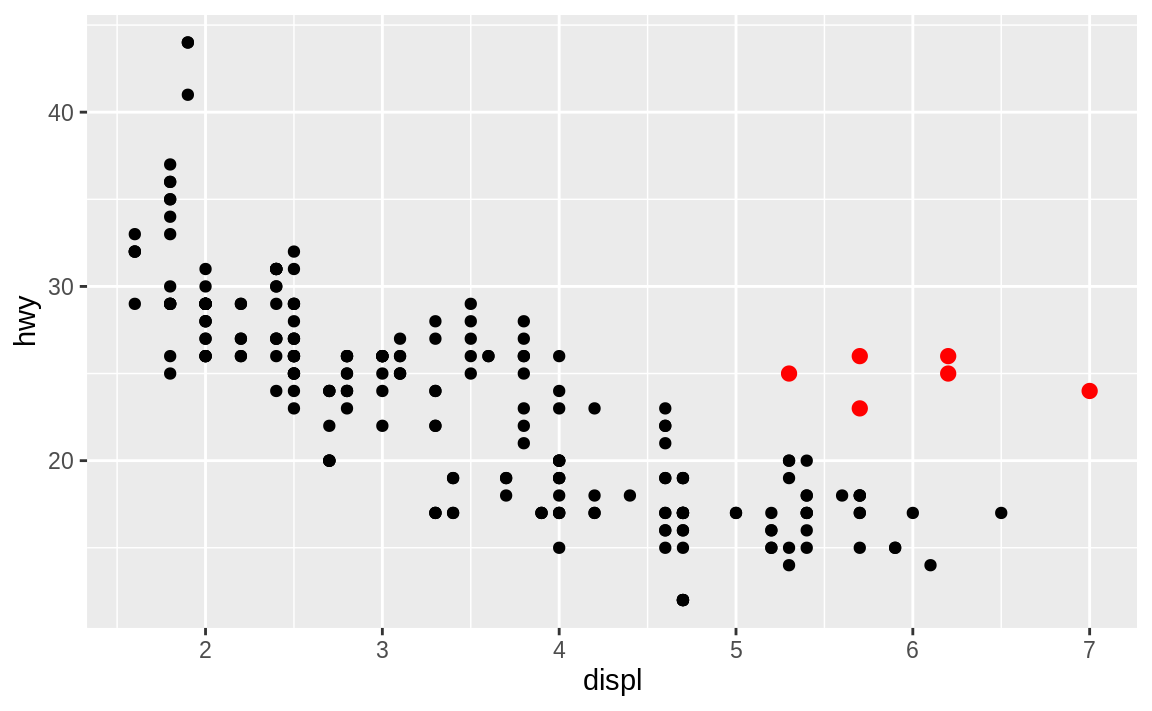
\includegraphics[width=3.125in,height=\textheight]{figures/outl.png}
\caption{Some cars have a higher mileage than we might expect}
\end{figure}

\end{frame}

\begin{frame}[fragile]{My first \texttt{ggplot()} revisited}
\protect\hypertarget{my-first-ggplot-revisited-1}{}

\begin{itemize}
\item
  The highlited cars may have some common caractheristic with respect to
  some other variable (e.g.~they might all be hybrids).
\item
  Lets try \texttt{class}, a variable that classifies cars into groups
  such as compact, midsize, and SUV.
\item
  We can add a third variable to a two dimensional scatterplot by
  mapping it to an aesthetic.
\end{itemize}

\end{frame}

\begin{frame}[fragile]{The color aesthetic}
\protect\hypertarget{the-color-aesthetic}{}

For example, we can map the color of the points to the \texttt{class}
variable, so that the graph reveals the class of each car:

\begin{Shaded}
\begin{Highlighting}[]
\KeywordTok{ggplot}\NormalTok{(}\DataTypeTok{data =}\NormalTok{ mpg) }\OperatorTok{+}
\StringTok{  }\KeywordTok{geom_point}\NormalTok{(}\KeywordTok{aes}\NormalTok{(}\DataTypeTok{x =}\NormalTok{ displ, }\DataTypeTok{y =}\NormalTok{ hwy, }\DataTypeTok{color =}\NormalTok{ class))}
\end{Highlighting}
\end{Shaded}

\end{frame}

\begin{frame}{The color aesthetic}
\protect\hypertarget{the-color-aesthetic-1}{}

\begin{center}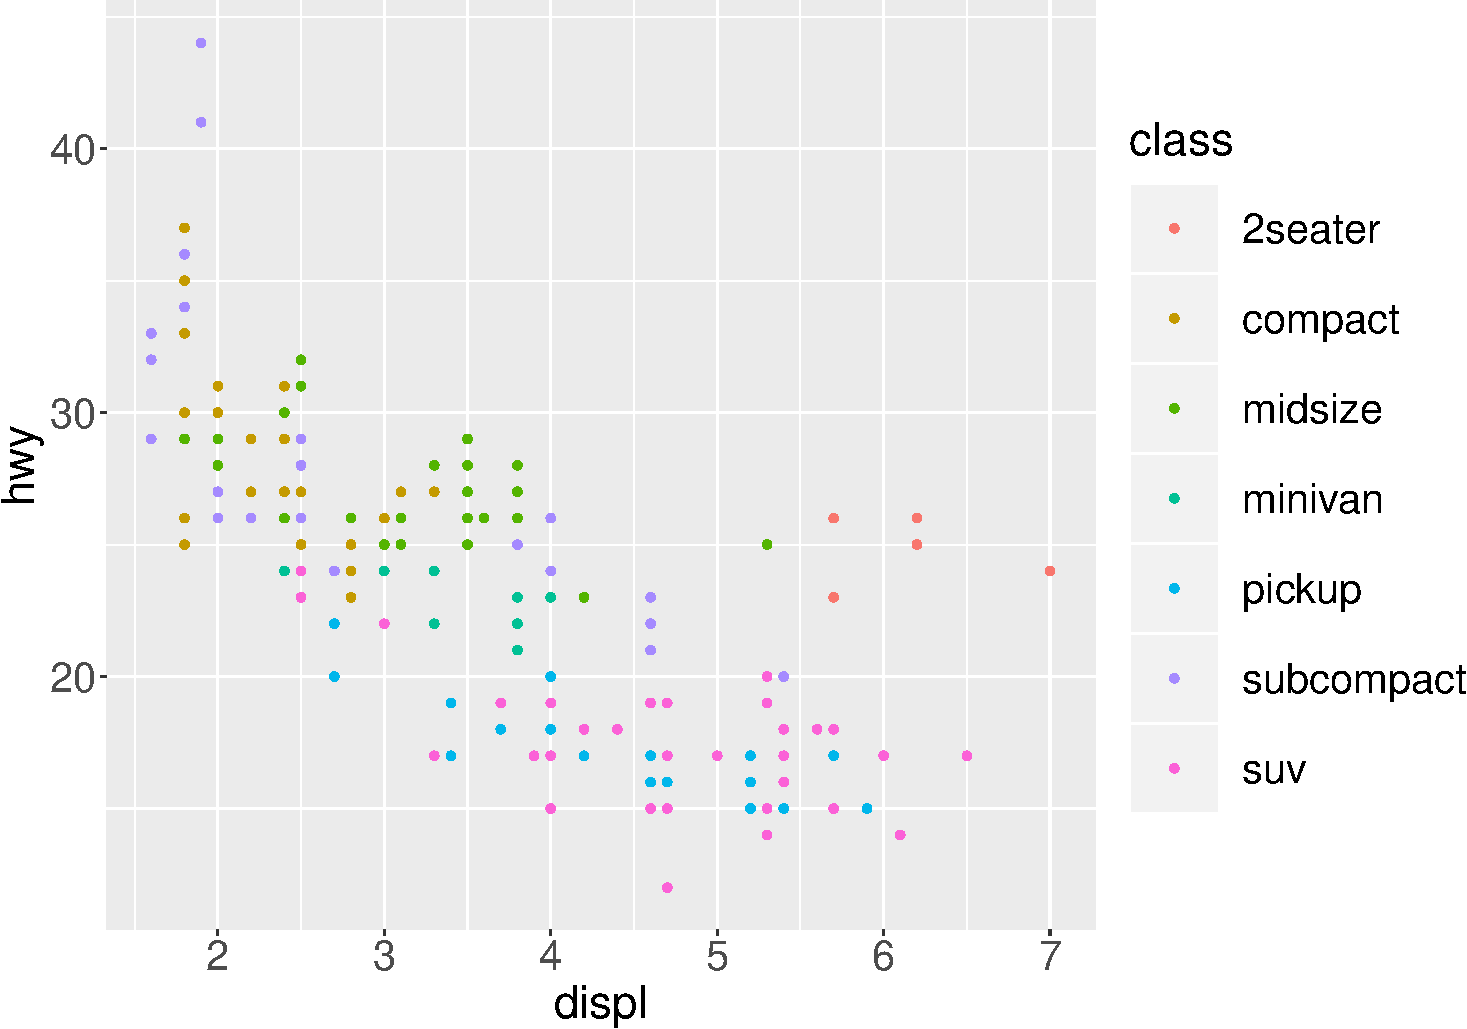
\includegraphics[height=200px]{data-visualization_files/figure-beamer/unnamed-chunk-8-1} \end{center}

\end{frame}

\begin{frame}[fragile]{The color aesthetic}
\protect\hypertarget{the-color-aesthetic-2}{}

Now we know that all but one of the highlited cars are two-seater cars!
Let's find their model and manufacturer:

\begin{Shaded}
\begin{Highlighting}[]
\KeywordTok{subset}\NormalTok{(mpg, class }\OperatorTok{==}\StringTok{ "2seater"}\NormalTok{, }
       \DataTypeTok{select =} \KeywordTok{c}\NormalTok{(}\StringTok{"manufacturer"}\NormalTok{, }\StringTok{"model"}\NormalTok{, }\StringTok{"year"}\NormalTok{))}
\end{Highlighting}
\end{Shaded}

\begin{verbatim}
## # A tibble: 5 x 3
##   manufacturer model     year
##   <chr>        <chr>    <int>
## 1 chevrolet    corvette  1999
## 2 chevrolet    corvette  1999
## 3 chevrolet    corvette  2008
## 4 chevrolet    corvette  2008
## 5 chevrolet    corvette  2008
\end{verbatim}

\end{frame}

\begin{frame}{The color aesthetic}
\protect\hypertarget{the-color-aesthetic-3}{}

\begin{itemize}
\item
  These cars are, in fact, sports cars!
\item
  Sports cars have large engines like SUVs and pickup trucks, but small
  bodies like midsize and compact cars, which improves their gas
  mileage.
\end{itemize}

\begin{figure}
\centering
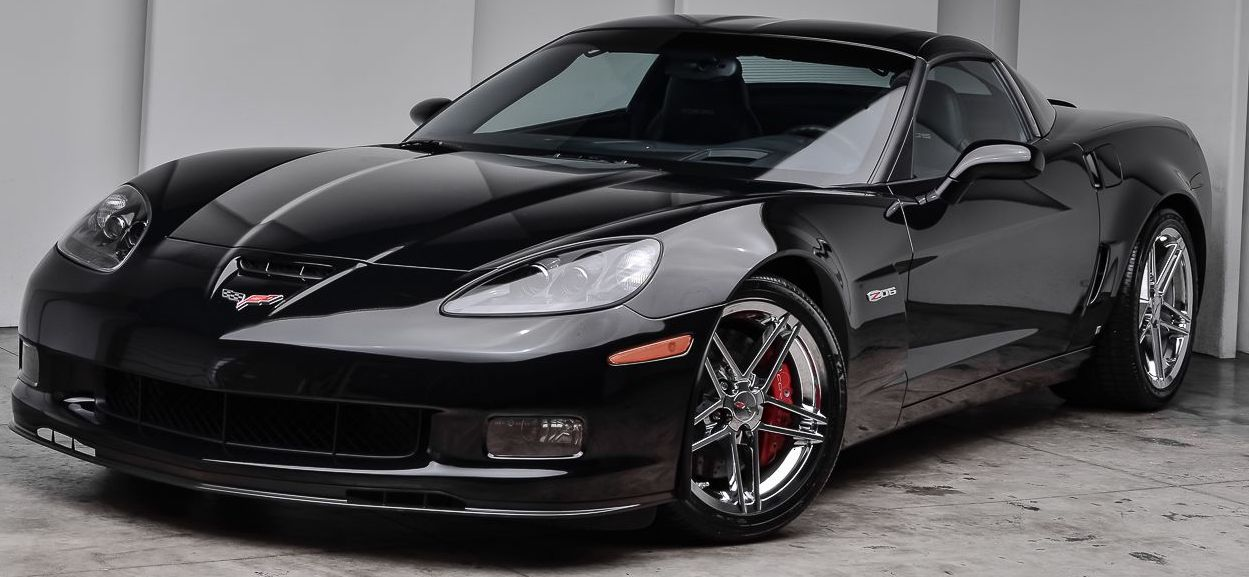
\includegraphics[width=2.60417in,height=\textheight]{figures/cc.jpg}
\caption{2008 Chevrolet Corvette}
\end{figure}

\end{frame}

\begin{frame}[fragile]{The size aesthetic}
\protect\hypertarget{the-size-aesthetic}{}

Now let´s map \texttt{class} to the size aesthetic:

\begin{Shaded}
\begin{Highlighting}[]
\KeywordTok{ggplot}\NormalTok{(}\DataTypeTok{data =}\NormalTok{ mpg) }\OperatorTok{+}
\StringTok{  }\KeywordTok{geom_point}\NormalTok{(}\KeywordTok{aes}\NormalTok{(}\DataTypeTok{x =}\NormalTok{ displ, }\DataTypeTok{y =}\NormalTok{ hwy, }\DataTypeTok{size =}\NormalTok{ class))}
\end{Highlighting}
\end{Shaded}

\end{frame}

\begin{frame}{The size aesthetic}
\protect\hypertarget{the-size-aesthetic-1}{}

\begin{center}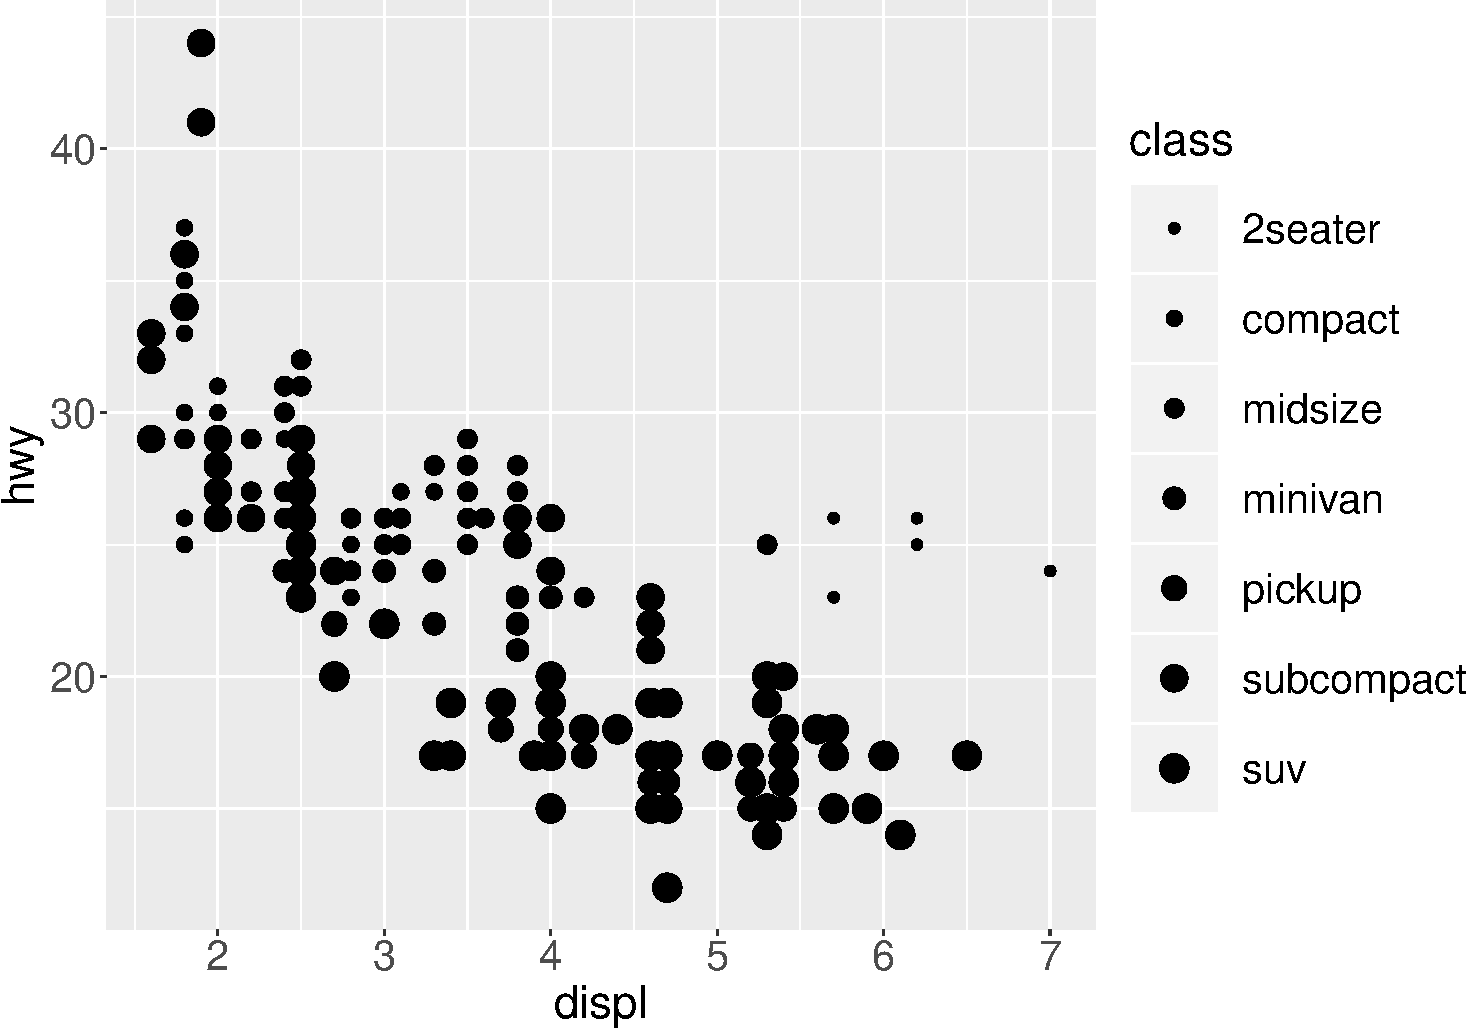
\includegraphics[height=200px]{data-visualization_files/figure-beamer/unnamed-chunk-11-1} \end{center}

\end{frame}

\begin{frame}[fragile]{The size aesthetic}
\protect\hypertarget{the-size-aesthetic-2}{}

\begin{itemize}
\item
  Each level of the \texttt{class} variable is assigned to a different
  size.
\item
  This plot, however, came with a warning message:
\end{itemize}

\begin{Shaded}
\begin{Highlighting}[]
\CommentTok{#> Using size for a discrete variable is not advised.}
\end{Highlighting}
\end{Shaded}

\begin{itemize}
\item
  This is because mapping an unordered variable (\texttt{class}) to
  ordered aesthetic (\texttt{size}) is not a good idea.
\item
  Ordered aesthetics, like \texttt{size} and \texttt{alpha}, are more
  appropriate for continuous variables.
\end{itemize}

\end{frame}

\begin{frame}[fragile]{The alpha aesthetic}
\protect\hypertarget{the-alpha-aesthetic}{}

The \texttt{alpha} aesthetic changes the transparency of the points:

\begin{Shaded}
\begin{Highlighting}[]
\KeywordTok{ggplot}\NormalTok{(}\DataTypeTok{data =}\NormalTok{ mpg) }\OperatorTok{+}
\StringTok{  }\KeywordTok{geom_point}\NormalTok{(}\KeywordTok{aes}\NormalTok{(}\DataTypeTok{x =}\NormalTok{ displ, }\DataTypeTok{y =}\NormalTok{ hwy, }\DataTypeTok{alpha =}\NormalTok{ class))}
\end{Highlighting}
\end{Shaded}

\end{frame}

\begin{frame}{The alpha aesthetic}
\protect\hypertarget{the-alpha-aesthetic-1}{}

\begin{center}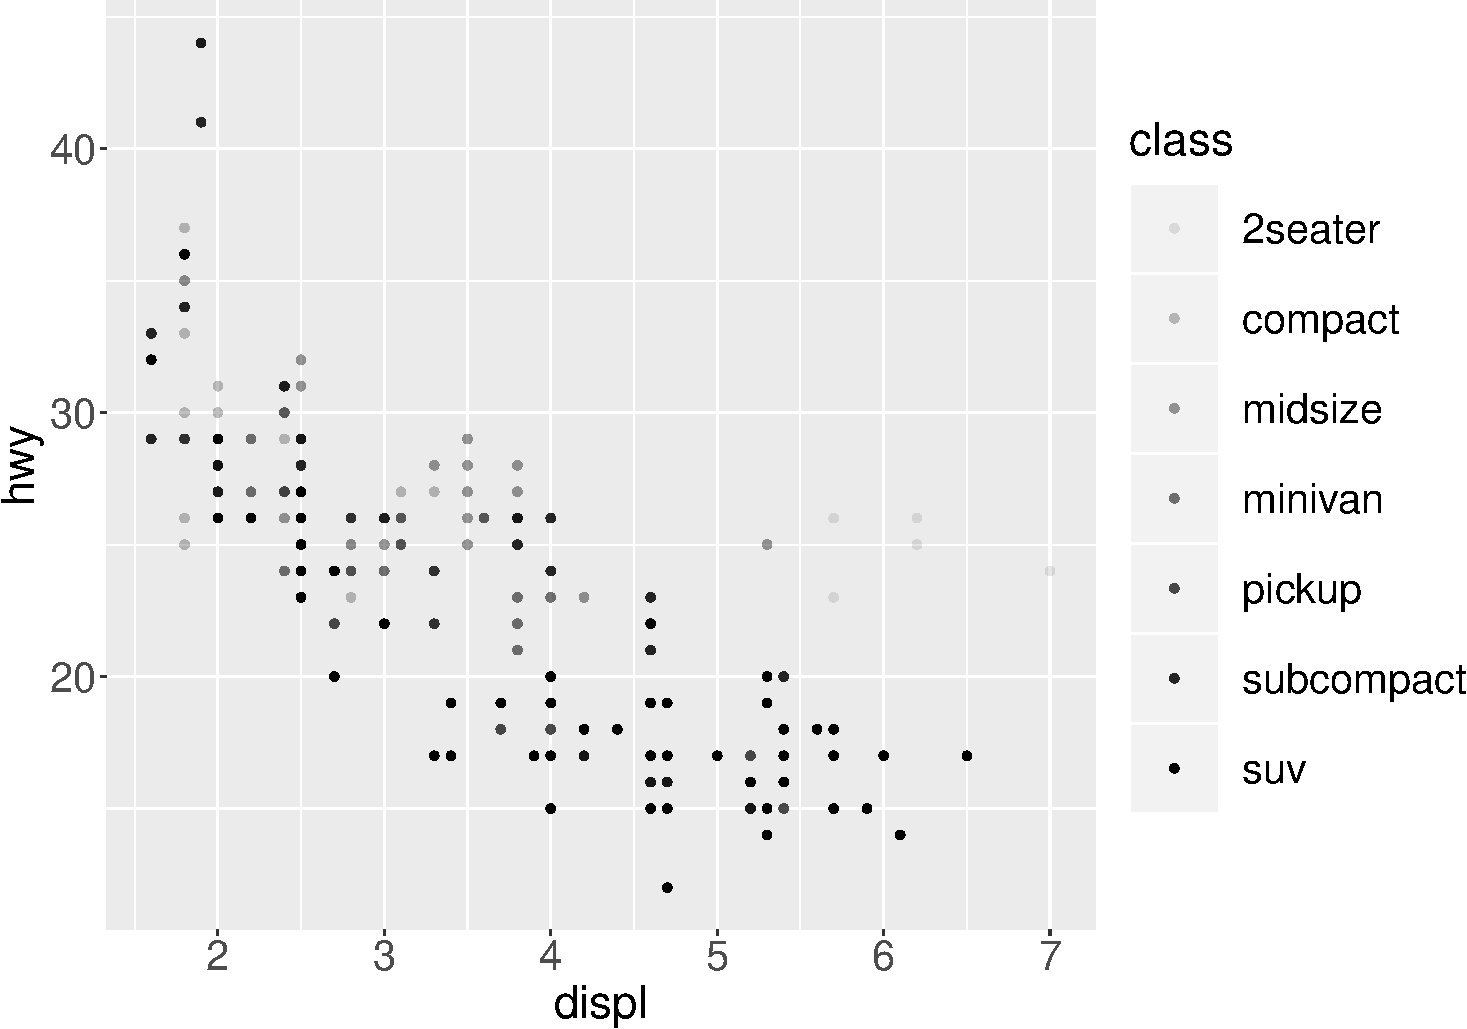
\includegraphics[height=200px]{data-visualization_files/figure-beamer/unnamed-chunk-14-1} \end{center}

\end{frame}

\begin{frame}[fragile]{The shape aesthetic}
\protect\hypertarget{the-shape-aesthetic}{}

The \texttt{shape} aesthetic changes the shape of the points:

\begin{Shaded}
\begin{Highlighting}[]
\KeywordTok{ggplot}\NormalTok{(}\DataTypeTok{data =}\NormalTok{ mpg) }\OperatorTok{+}
\StringTok{  }\KeywordTok{geom_point}\NormalTok{(}\KeywordTok{aes}\NormalTok{(}\DataTypeTok{x =}\NormalTok{ displ, }\DataTypeTok{y =}\NormalTok{ hwy, }\DataTypeTok{shape =}\NormalTok{ class))}
\end{Highlighting}
\end{Shaded}

\end{frame}

\begin{frame}{The shape aesthetic}
\protect\hypertarget{the-shape-aesthetic-1}{}

\begin{center}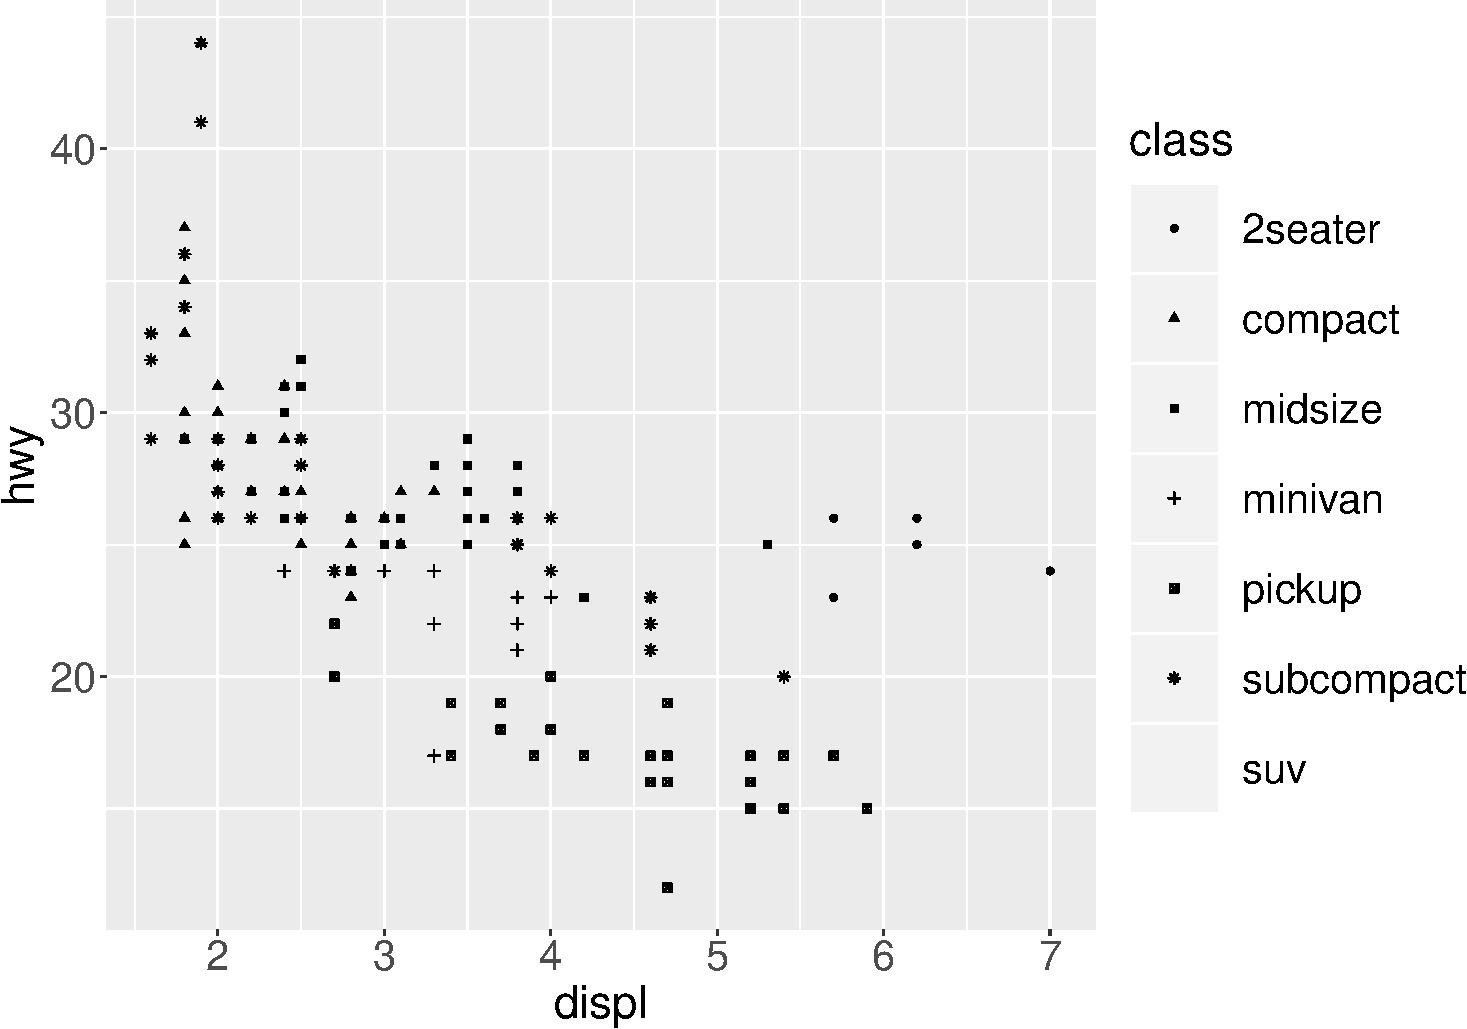
\includegraphics[height=200px]{data-visualization_files/figure-beamer/unnamed-chunk-16-1} \end{center}

\end{frame}

\begin{frame}[fragile]{The shape aesthetic}
\protect\hypertarget{the-shape-aesthetic-2}{}

\begin{itemize}
\item
  What happened to the SUVs?
\item
  By default ggplot2 uses only up to six shapes at a time.
\item
  This is because points become difficult to discriminate if we use too
  many shapes.
\item
  We can, however, use more than six shapes if we set them ``manually''
  with \texttt{scale\_shape\_manual()}.
\end{itemize}

\end{frame}

\begin{frame}{The shape aesthetic}
\protect\hypertarget{the-shape-aesthetic-3}{}

We can choose the following shapes of points by their number:

\begin{figure}
\centering
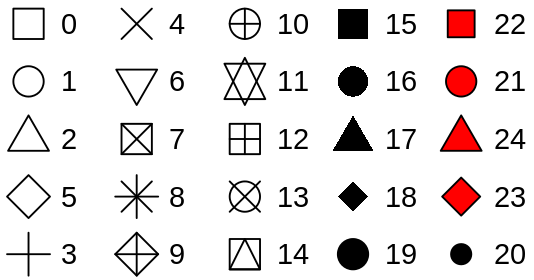
\includegraphics[width=2.08333in,height=\textheight]{figures/shapes-1}
\caption{R Built in shapes}
\end{figure}

\end{frame}

\begin{frame}[fragile]{The shape aesthetic}
\protect\hypertarget{the-shape-aesthetic-4}{}

Let's choose the first 7 shapes:

\begin{Shaded}
\begin{Highlighting}[]
\KeywordTok{ggplot}\NormalTok{(}\DataTypeTok{data =}\NormalTok{ mpg) }\OperatorTok{+}
\StringTok{  }\KeywordTok{geom_point}\NormalTok{(}\KeywordTok{aes}\NormalTok{(}\DataTypeTok{x =}\NormalTok{ displ, }\DataTypeTok{y =}\NormalTok{ hwy, }\DataTypeTok{shape =}\NormalTok{ class)) }\OperatorTok{+}
\StringTok{  }\KeywordTok{scale_shape_manual}\NormalTok{(}\DataTypeTok{values =} \DecValTok{0}\OperatorTok{:}\DecValTok{6}\NormalTok{)}
\end{Highlighting}
\end{Shaded}

\end{frame}

\begin{frame}{The shape aesthetic}
\protect\hypertarget{the-shape-aesthetic-5}{}

\begin{center}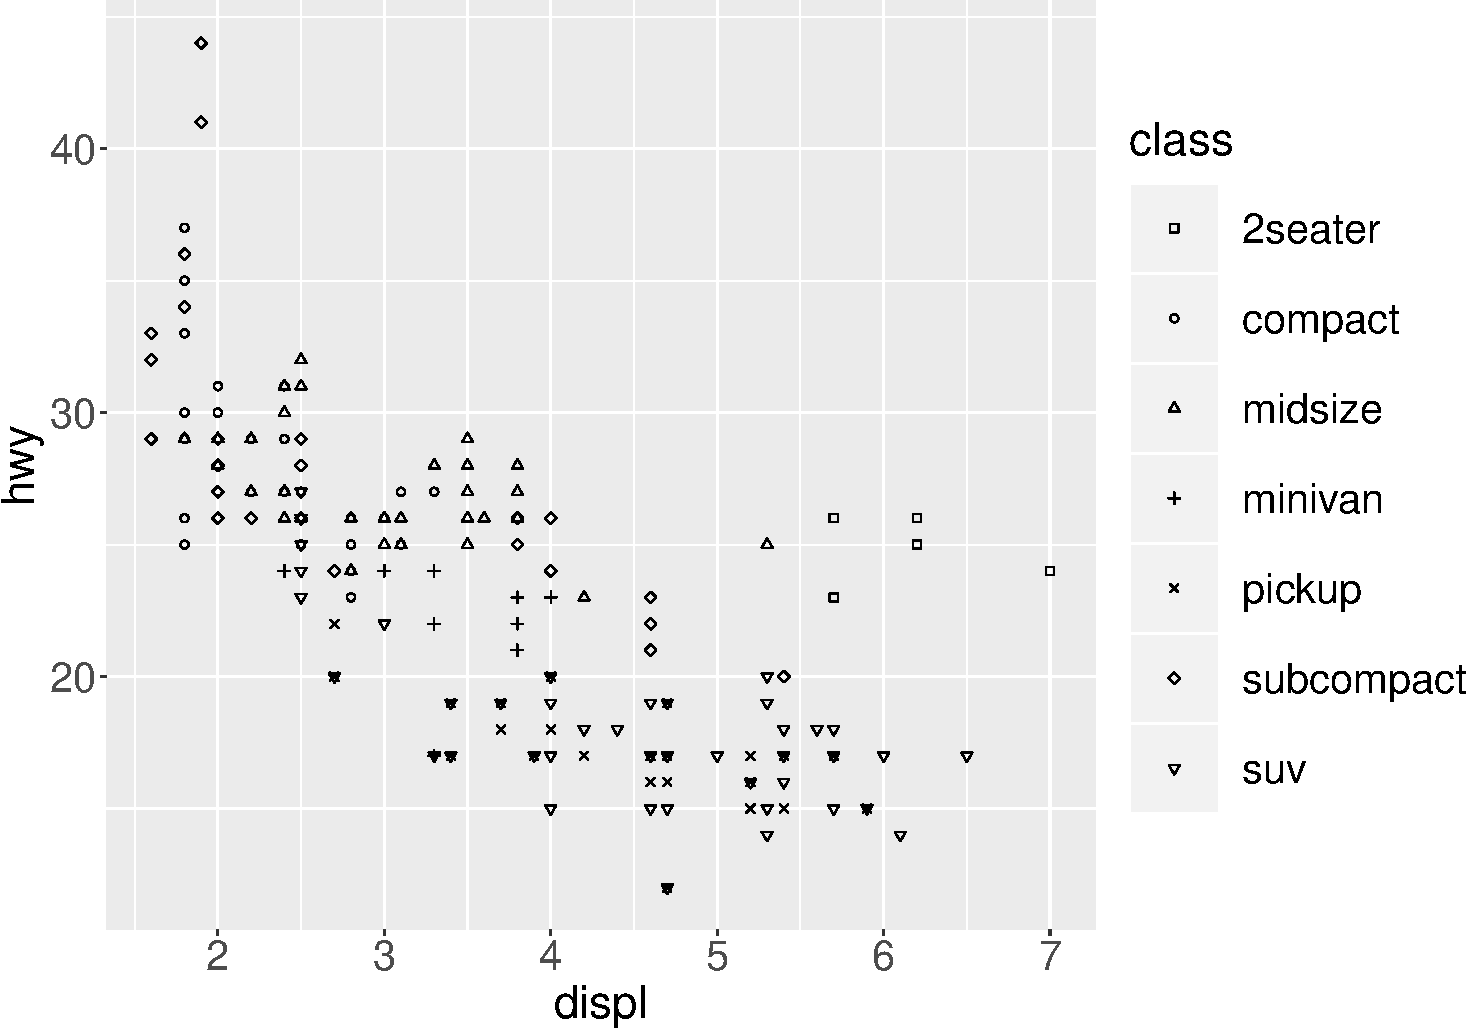
\includegraphics[height=200px]{data-visualization_files/figure-beamer/unnamed-chunk-18-1} \end{center}

\end{frame}

\begin{frame}[fragile]{Mapping one variable to two aesthetics}
\protect\hypertarget{mapping-one-variable-to-two-aesthetics}{}

\begin{itemize}
\item
  Mapping a single variable to multiple aesthetics is redundant, and
  should be avoided in most cases.
\item
  In this case, however, since we have many categories, it can improving
  visual discrimanation.
\item
  Let´s map \texttt{class} to \texttt{color} and \texttt{shape}:
\end{itemize}

\begin{Shaded}
\begin{Highlighting}[]
\KeywordTok{ggplot}\NormalTok{(}\DataTypeTok{data =}\NormalTok{ mpg) }\OperatorTok{+}
\StringTok{  }\KeywordTok{geom_point}\NormalTok{(}\KeywordTok{aes}\NormalTok{(}\DataTypeTok{x =}\NormalTok{ displ, }\DataTypeTok{y =}\NormalTok{ hwy, }
                 \DataTypeTok{shape =}\NormalTok{ class, }\DataTypeTok{color =}\NormalTok{ class)) }\OperatorTok{+}
\StringTok{  }\KeywordTok{scale_shape_manual}\NormalTok{(}\DataTypeTok{values =} \DecValTok{1}\OperatorTok{:}\DecValTok{7}\NormalTok{)}
\end{Highlighting}
\end{Shaded}

\end{frame}

\begin{frame}{Mapping one variable to two aesthetics}
\protect\hypertarget{mapping-one-variable-to-two-aesthetics-1}{}

\begin{center}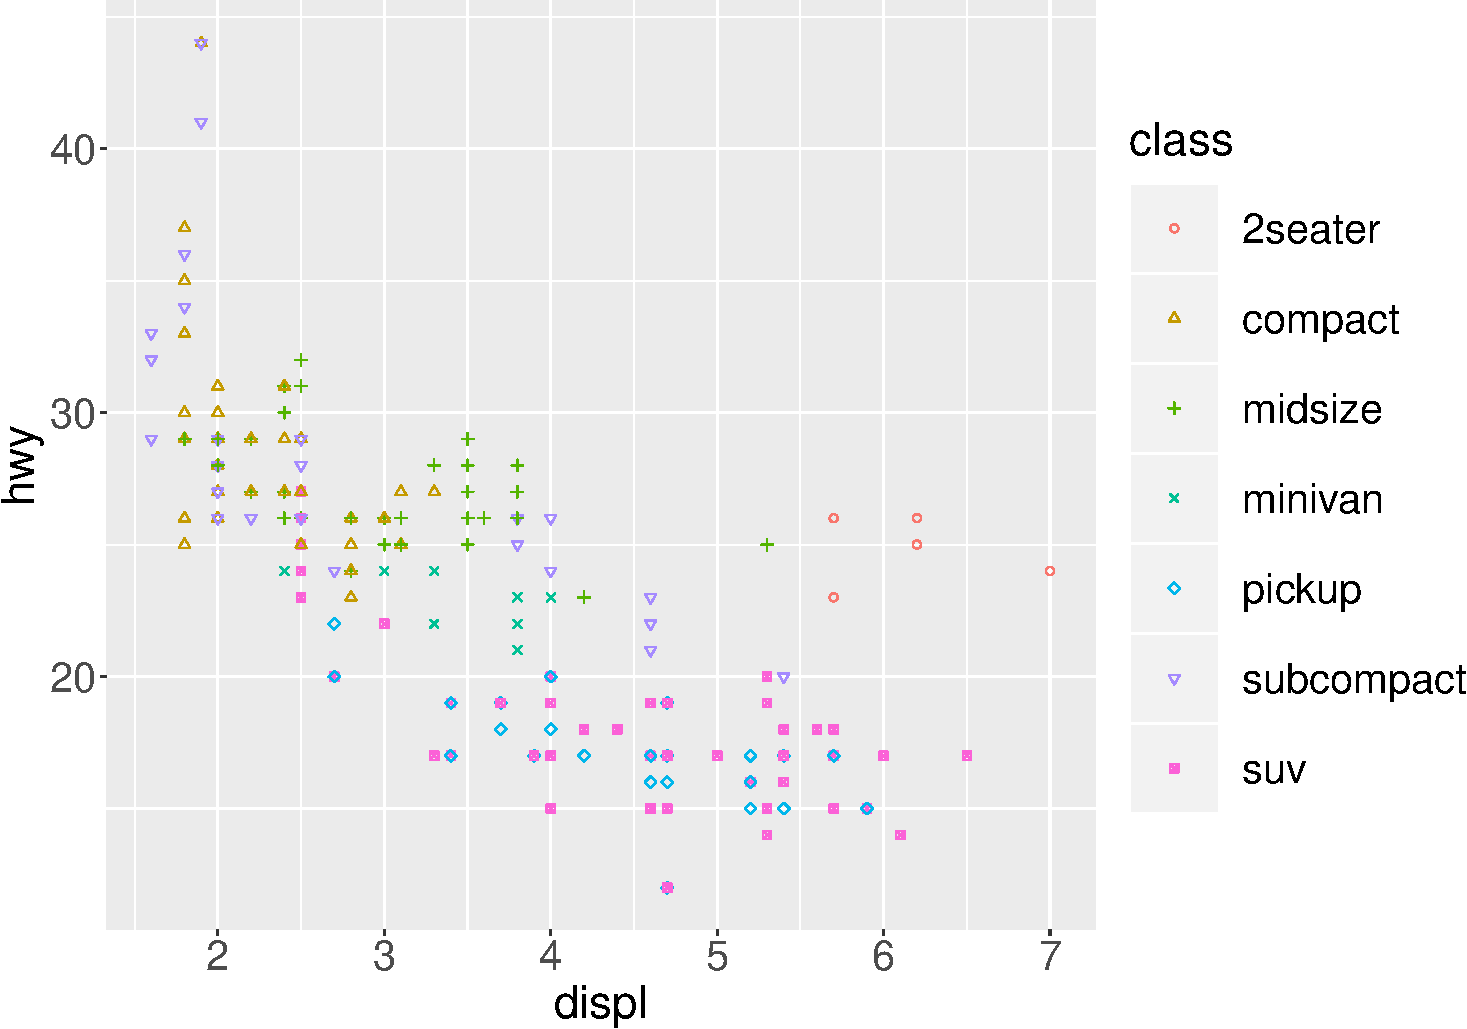
\includegraphics[height=200px]{data-visualization_files/figure-beamer/unnamed-chunk-20-1} \end{center}

\end{frame}

\begin{frame}[fragile]{Mapping continuous variables to aesthetics}
\protect\hypertarget{mapping-continuous-variables-to-aesthetics}{}

\begin{itemize}
\item
  So far we mapped \texttt{class}, a categorical variable, to the
  \texttt{color}, \texttt{size}, \texttt{shape} and \texttt{alpha}
  aesthetics of \texttt{geom\_point()}.
\item
  Now let´s map continuous variables to these aesthetics and see how
  they behaves differently for categorial versus continuous variables.
\item
  The variable \texttt{cty} (city miles per gallon) is a continuous
  variable.
\end{itemize}

\end{frame}

\begin{frame}[fragile]{Mapping continuous variables to aesthetics}
\protect\hypertarget{mapping-continuous-variables-to-aesthetics-1}{}

Let's map \texttt{cty} to the \texttt{color} aesthetic:

\begin{Shaded}
\begin{Highlighting}[]
\KeywordTok{ggplot}\NormalTok{(mpg) }\OperatorTok{+}
\StringTok{  }\KeywordTok{geom_point}\NormalTok{(}\KeywordTok{aes}\NormalTok{(}\DataTypeTok{x =}\NormalTok{ displ,}\DataTypeTok{y =}\NormalTok{ hwy, }\DataTypeTok{colour =}\NormalTok{ cty))}
\end{Highlighting}
\end{Shaded}

\end{frame}

\begin{frame}{Mapping continuous variables to aesthetics}
\protect\hypertarget{mapping-continuous-variables-to-aesthetics-2}{}

\begin{center}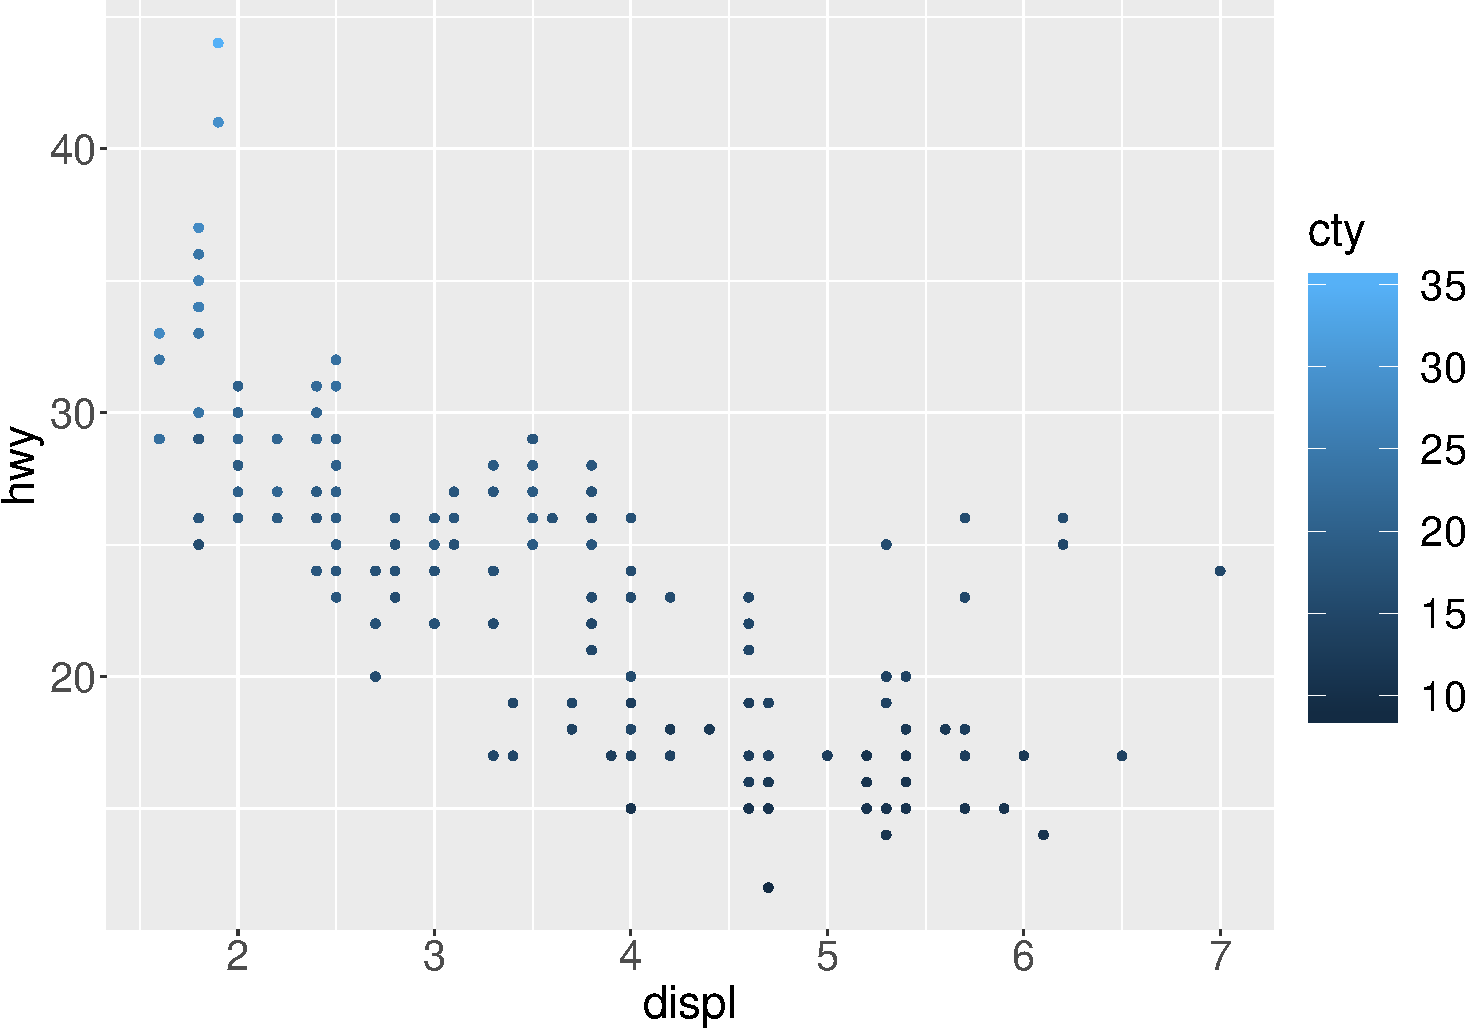
\includegraphics[height=200px]{data-visualization_files/figure-beamer/unnamed-chunk-22-1} \end{center}

\end{frame}

\begin{frame}[fragile]{Mapping continuous variables to aesthetics}
\protect\hypertarget{mapping-continuous-variables-to-aesthetics-3}{}

Now let's map \texttt{cty} to the \texttt{size} aesthetic:

\begin{Shaded}
\begin{Highlighting}[]
\KeywordTok{ggplot}\NormalTok{(mpg) }\OperatorTok{+}\StringTok{ }
\StringTok{  }\KeywordTok{geom_point}\NormalTok{(}\KeywordTok{aes}\NormalTok{(}\DataTypeTok{x =}\NormalTok{ displ, }\DataTypeTok{y =}\NormalTok{ hwy, }\DataTypeTok{size =}\NormalTok{ cty))}
\end{Highlighting}
\end{Shaded}

\end{frame}

\begin{frame}{Mapping continuous variables to aesthetics}
\protect\hypertarget{mapping-continuous-variables-to-aesthetics-4}{}

\begin{center}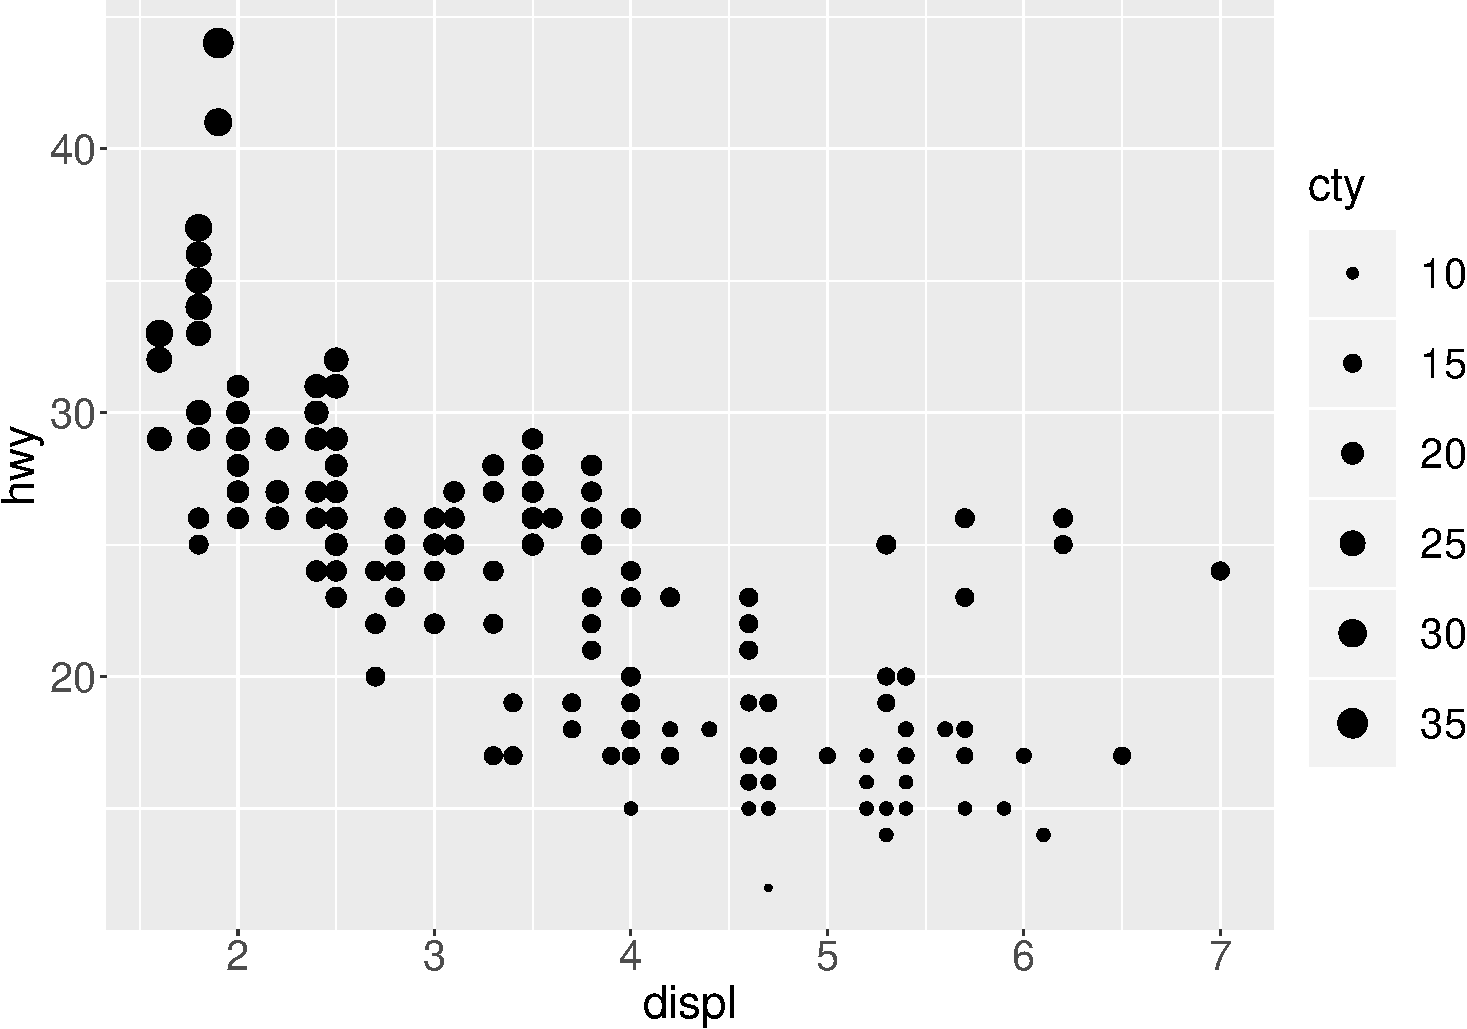
\includegraphics[height=200px]{data-visualization_files/figure-beamer/unnamed-chunk-24-1} \end{center}

\end{frame}

\begin{frame}[fragile]{Mapping continuous variables to aesthetics}
\protect\hypertarget{mapping-continuous-variables-to-aesthetics-5}{}

Now let's map \texttt{cty} to the \texttt{alpha} aesthetic:

\begin{Shaded}
\begin{Highlighting}[]
\KeywordTok{ggplot}\NormalTok{(mpg) }\OperatorTok{+}\StringTok{ }
\StringTok{  }\KeywordTok{geom_point}\NormalTok{(}\KeywordTok{aes}\NormalTok{(}\DataTypeTok{x =}\NormalTok{ displ, }\DataTypeTok{y =}\NormalTok{ hwy, }\DataTypeTok{alpha =}\NormalTok{ cty)) }
\end{Highlighting}
\end{Shaded}

\end{frame}

\begin{frame}{Mapping continuous variables to aesthetics}
\protect\hypertarget{mapping-continuous-variables-to-aesthetics-6}{}

\begin{center}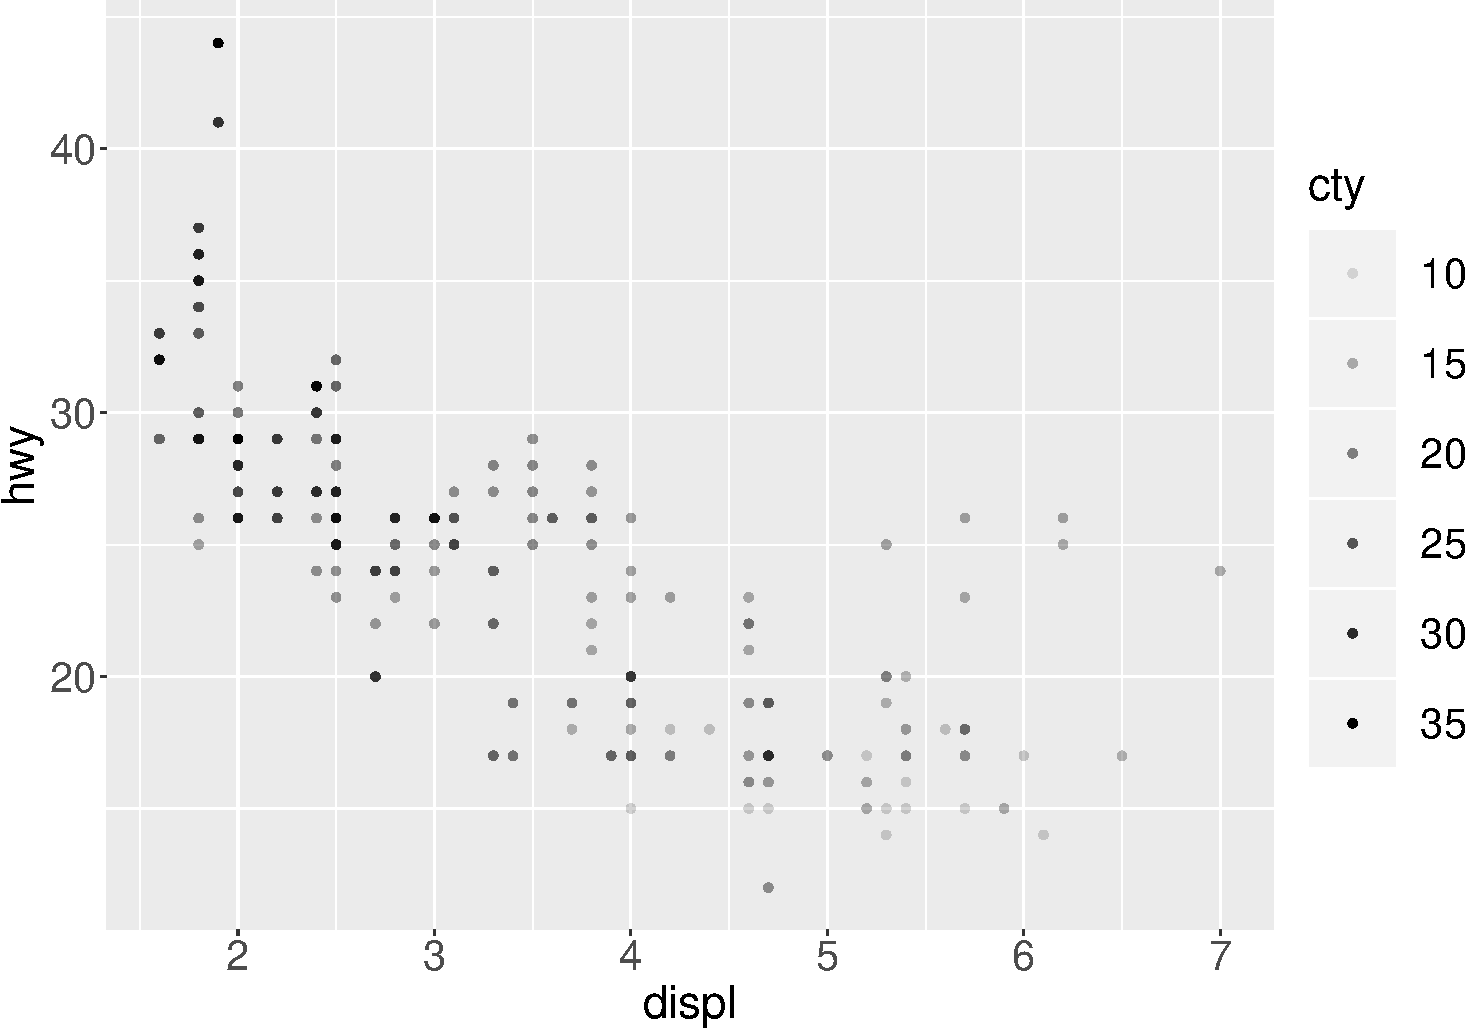
\includegraphics[height=200px]{data-visualization_files/figure-beamer/unnamed-chunk-26-1} \end{center}

\end{frame}

\begin{frame}[fragile]{Mapping continuous variables to aesthetics}
\protect\hypertarget{mapping-continuous-variables-to-aesthetics-7}{}

And finally let's map \texttt{cty} to the \texttt{shape} aesthetic:

\begin{Shaded}
\begin{Highlighting}[]
\KeywordTok{ggplot}\NormalTok{(mpg) }\OperatorTok{+}\StringTok{ }
\StringTok{  }\KeywordTok{geom_point}\NormalTok{(}\KeywordTok{aes}\NormalTok{(}\DataTypeTok{x =}\NormalTok{ displ, }\DataTypeTok{y =}\NormalTok{ hwy, }\DataTypeTok{shape =}\NormalTok{ cty))     }

\CommentTok{#> Error: A continuous variable can not be mapped to }
\CommentTok{#> shape}
\end{Highlighting}
\end{Shaded}

\end{frame}

\begin{frame}{Aesthetic mappings: categorical vs continuous variables}
\protect\hypertarget{aesthetic-mappings-categorical-vs-continuous-variables}{}

\textbf{Color} and \textbf{alpha} aesthetics:

\begin{itemize}
\item
  Each level of a categorival variable is assgined to a different
  (discrete) color.
\item
  The color of the points vary continuously from light to dark as a
  function of the values of a continuous variables.
\end{itemize}

\textbf{Size} aestietic:

\begin{itemize}
\item
  Each level of a categorival variable is assigned to a different
  (discrete) size.
\item
  The size of the points vary continuously as a function of the values
  of a continuous variables.
\end{itemize}

\end{frame}

\begin{frame}{Aesthetic mappings: categorical vs continuous variables}
\protect\hypertarget{aesthetic-mappings-categorical-vs-continuous-variables-1}{}

\textbf{Shape} aestietic:

\begin{itemize}
\item
  A different shape is assigned to each level of a categorical value.
\item
  The shape aesthetic can not be mapped to continuous variables.
\end{itemize}

\end{frame}

\begin{frame}[fragile]{The \texttt{linetype} aesthetic}
\protect\hypertarget{the-linetype-aesthetic}{}

\texttt{geom\_smooth()} draws a different type of line for each level of
the variable that is mapped to the \texttt{linetype} aesthetic:

\begin{Shaded}
\begin{Highlighting}[]
\KeywordTok{ggplot}\NormalTok{(}\DataTypeTok{data =}\NormalTok{ mpg) }\OperatorTok{+}\StringTok{ }
\StringTok{  }\KeywordTok{geom_smooth}\NormalTok{(}\KeywordTok{aes}\NormalTok{(}\DataTypeTok{x =}\NormalTok{ displ, }\DataTypeTok{y =}\NormalTok{ hwy, }\DataTypeTok{linetype =}\NormalTok{ drv))}
\end{Highlighting}
\end{Shaded}

\end{frame}

\begin{frame}{The \texttt{linetype} aesthetic}
\protect\hypertarget{the-linetype-aesthetic-1}{}

\begin{center}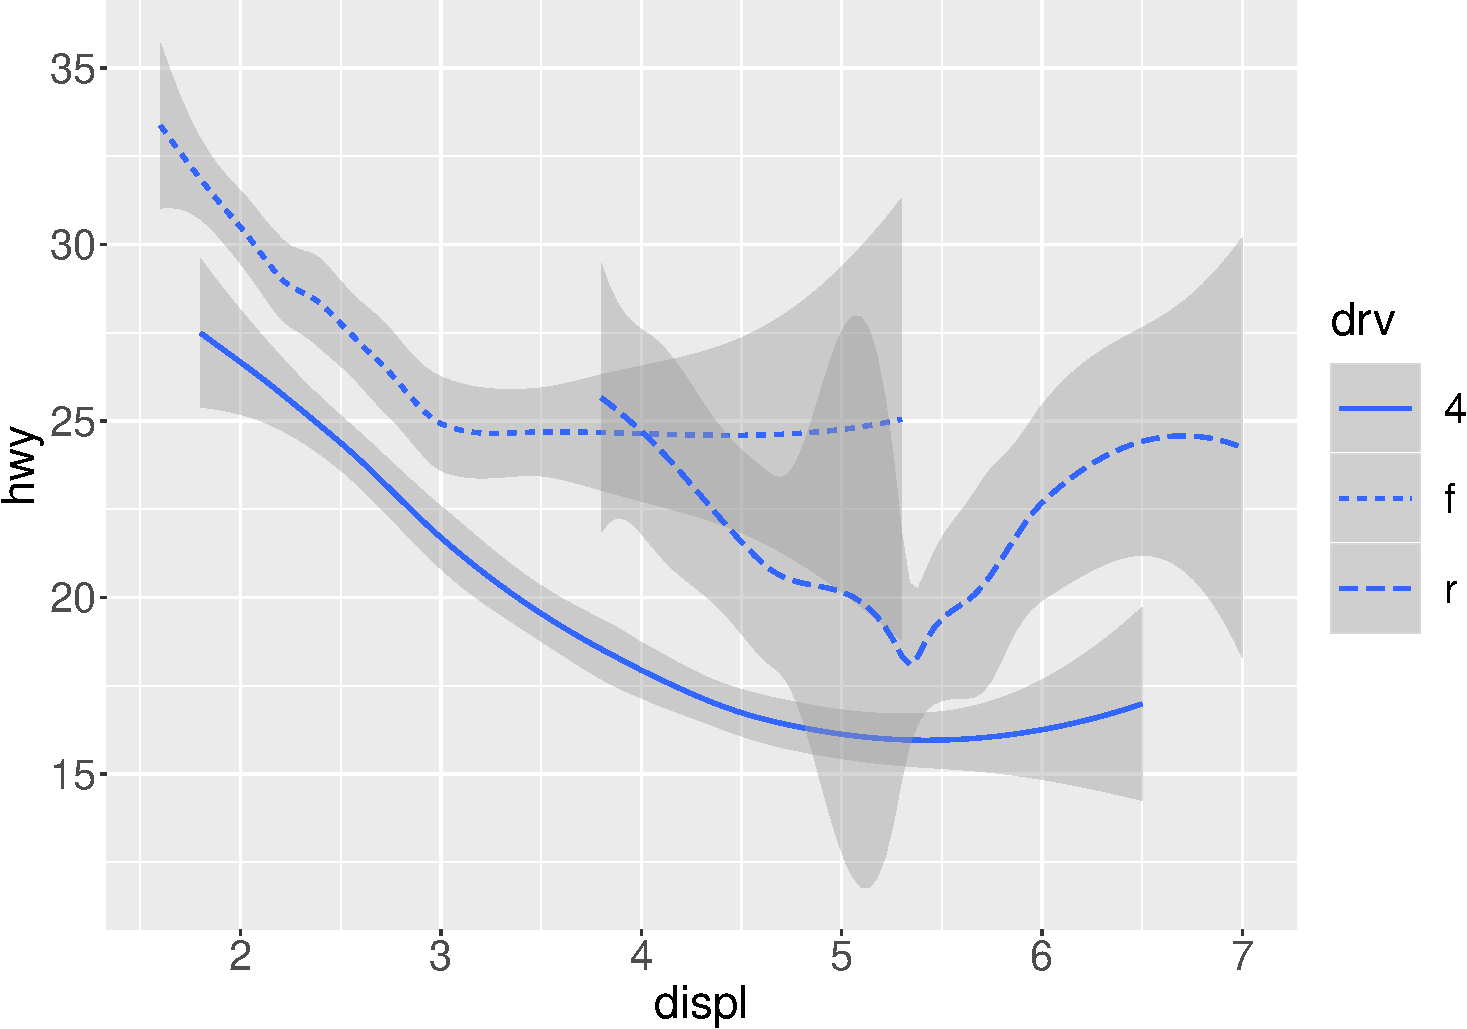
\includegraphics[height=200px]{data-visualization_files/figure-beamer/unnamed-chunk-29-1} \end{center}

\end{frame}

\begin{frame}{The \texttt{linetype} aesthetic}
\protect\hypertarget{the-linetype-aesthetic-2}{}

\begin{itemize}
\tightlist
\item
  The linetype aesthetic automatically adds a legend.
\item
  The linetype aesthetic can not be mapped to continuous variables.
\end{itemize}

\end{frame}

\begin{frame}[fragile]{The \texttt{group} aesthetic}
\protect\hypertarget{the-group-aesthetic}{}

\begin{itemize}
\item
  The \texttt{group} aesthetic also draws a separate object for each
  level of a discrete variable.
\item
  The \texttt{group} aesthetic does not add a legend or any other
  distinguishing feature.
\end{itemize}

\end{frame}

\begin{frame}[fragile]{The \texttt{group} aesthetic}
\protect\hypertarget{the-group-aesthetic-1}{}

\begin{Shaded}
\begin{Highlighting}[]
\NormalTok{p1 <-}\StringTok{ }\KeywordTok{ggplot}\NormalTok{(}\DataTypeTok{data =}\NormalTok{ mpg) }\OperatorTok{+}
\StringTok{  }\KeywordTok{geom_smooth}\NormalTok{(}\KeywordTok{aes}\NormalTok{(}\DataTypeTok{x =}\NormalTok{ displ, }\DataTypeTok{y =}\NormalTok{ hwy))}

\NormalTok{p2 <-}\StringTok{ }\KeywordTok{ggplot}\NormalTok{(}\DataTypeTok{data =}\NormalTok{ mpg) }\OperatorTok{+}
\StringTok{  }\KeywordTok{geom_smooth}\NormalTok{(}\KeywordTok{aes}\NormalTok{(}\DataTypeTok{x =}\NormalTok{ displ, }\DataTypeTok{y =}\NormalTok{ hwy, }\DataTypeTok{group =}\NormalTok{ drv))}
\end{Highlighting}
\end{Shaded}

\end{frame}

\begin{frame}{The \texttt{group} aesthetic}
\protect\hypertarget{the-group-aesthetic-2}{}

\begin{center}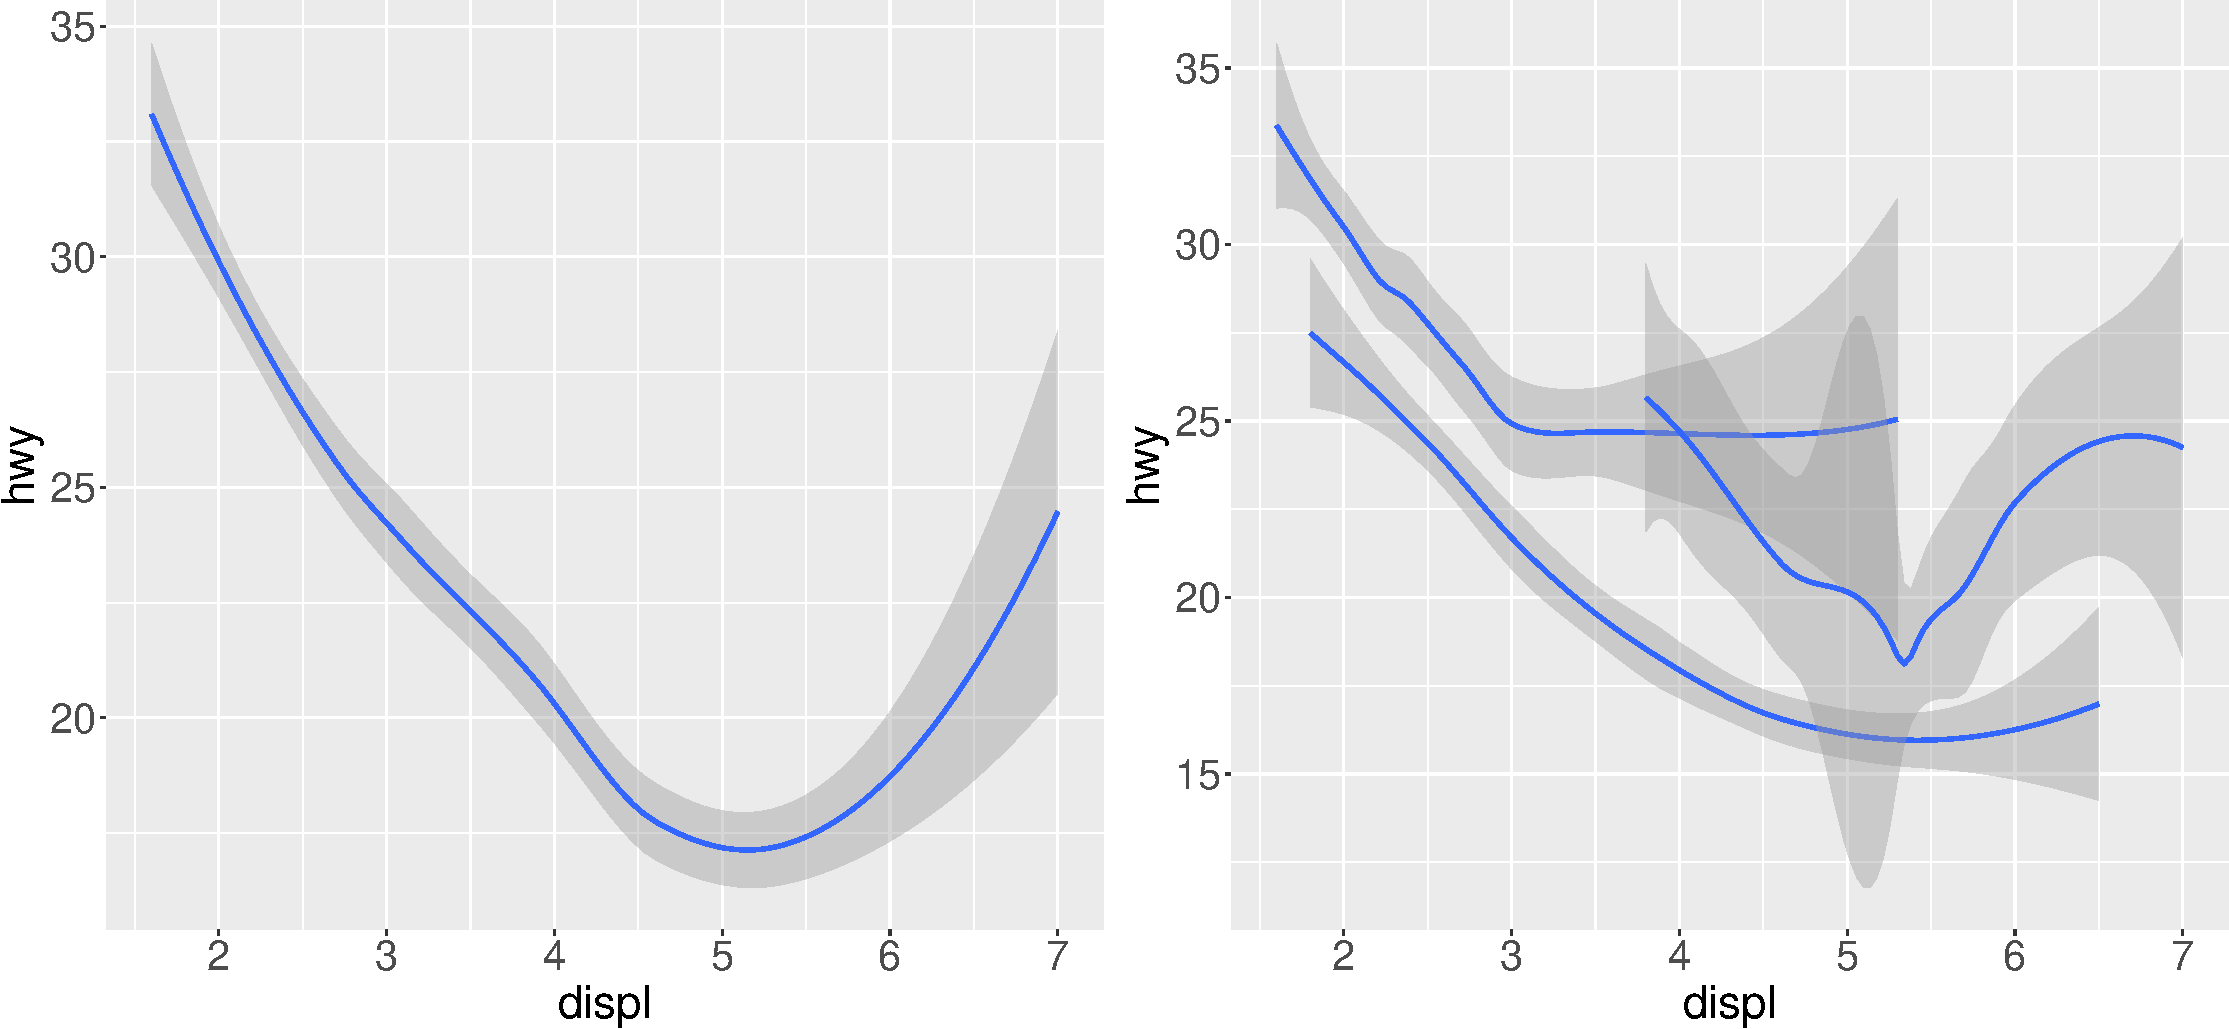
\includegraphics[height=150px]{data-visualization_files/figure-beamer/unnamed-chunk-31-1} \end{center}

\end{frame}

\begin{frame}[fragile]{\texttt{group} vs \texttt{linetype}}
\protect\hypertarget{group-vs-linetype}{}

\begin{Shaded}
\begin{Highlighting}[]
\KeywordTok{ggplot}\NormalTok{(}\DataTypeTok{data =}\NormalTok{ mpg) }\OperatorTok{+}
\StringTok{  }\KeywordTok{geom_smooth}\NormalTok{(}\KeywordTok{aes}\NormalTok{(}\DataTypeTok{x =}\NormalTok{ displ, }\DataTypeTok{y =}\NormalTok{ hwy, }\DataTypeTok{group =}\NormalTok{ drv))}

\KeywordTok{ggplot}\NormalTok{(}\DataTypeTok{data =}\NormalTok{ mpg) }\OperatorTok{+}
\StringTok{  }\KeywordTok{geom_smooth}\NormalTok{(}\KeywordTok{aes}\NormalTok{(}\DataTypeTok{x =}\NormalTok{ displ, }\DataTypeTok{y =}\NormalTok{ hwy, }\DataTypeTok{linetype =}\NormalTok{ drv))}
\end{Highlighting}
\end{Shaded}

\end{frame}

\begin{frame}{\texttt{group} vs \texttt{linetype}}
\protect\hypertarget{group-vs-linetype-1}{}

\begin{center}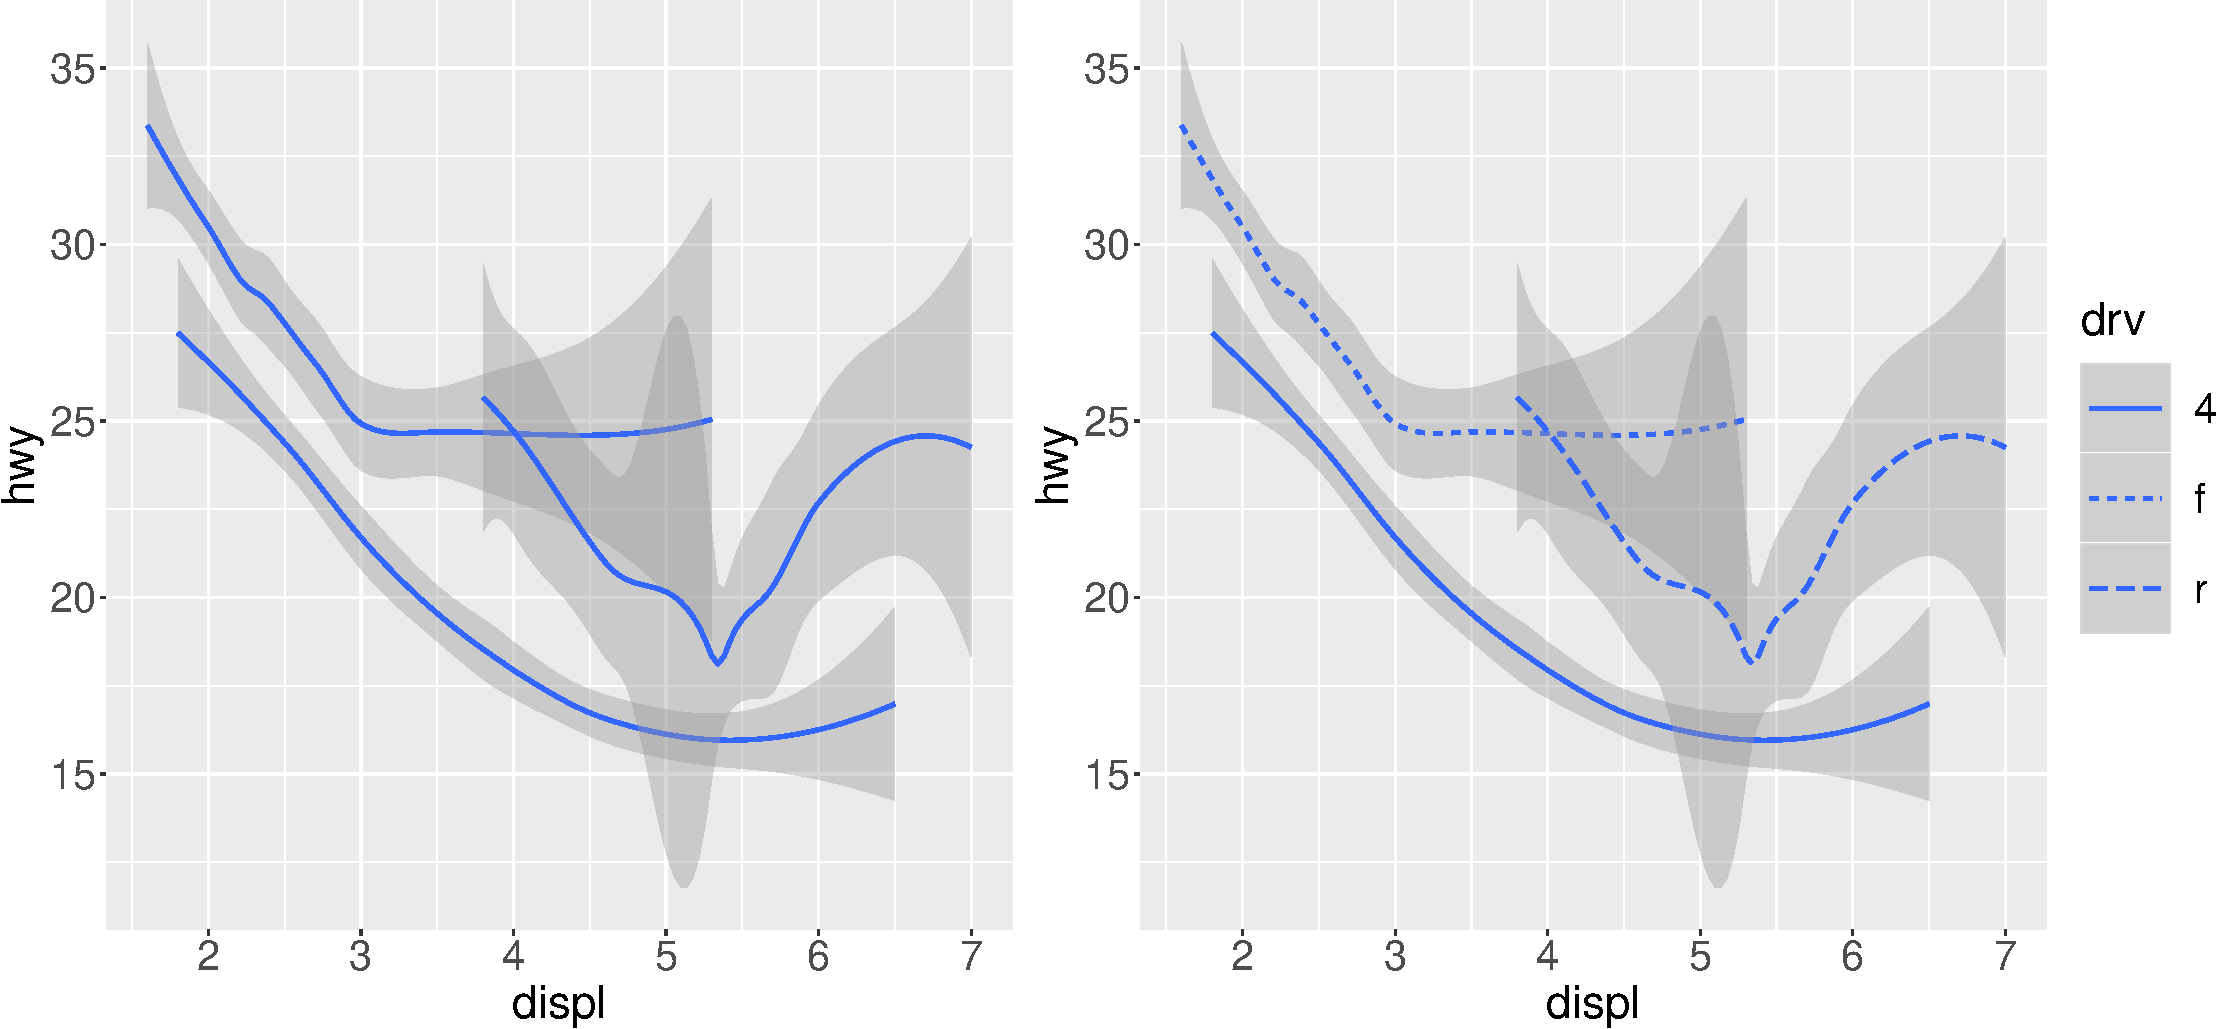
\includegraphics[height=150px]{data-visualization_files/figure-beamer/unnamed-chunk-33-1} \end{center}

\end{frame}

\begin{frame}[fragile]{\texttt{group} vs \texttt{color}}
\protect\hypertarget{group-vs-color}{}

\begin{Shaded}
\begin{Highlighting}[]
\KeywordTok{ggplot}\NormalTok{(}\DataTypeTok{data =}\NormalTok{ mpg) }\OperatorTok{+}
\StringTok{  }\KeywordTok{geom_smooth}\NormalTok{(}\KeywordTok{aes}\NormalTok{(}\DataTypeTok{x =}\NormalTok{ displ, }\DataTypeTok{y =}\NormalTok{ hwy, }\DataTypeTok{group =}\NormalTok{ drv))}

\KeywordTok{ggplot}\NormalTok{(}\DataTypeTok{data =}\NormalTok{ mpg) }\OperatorTok{+}
\StringTok{  }\KeywordTok{geom_smooth}\NormalTok{(}\KeywordTok{aes}\NormalTok{(}\DataTypeTok{x =}\NormalTok{ displ, }\DataTypeTok{y =}\NormalTok{ hwy, }\DataTypeTok{color =}\NormalTok{ drv))}
\end{Highlighting}
\end{Shaded}

\end{frame}

\begin{frame}{\texttt{group} vs \texttt{color}}
\protect\hypertarget{group-vs-color-1}{}

\begin{center}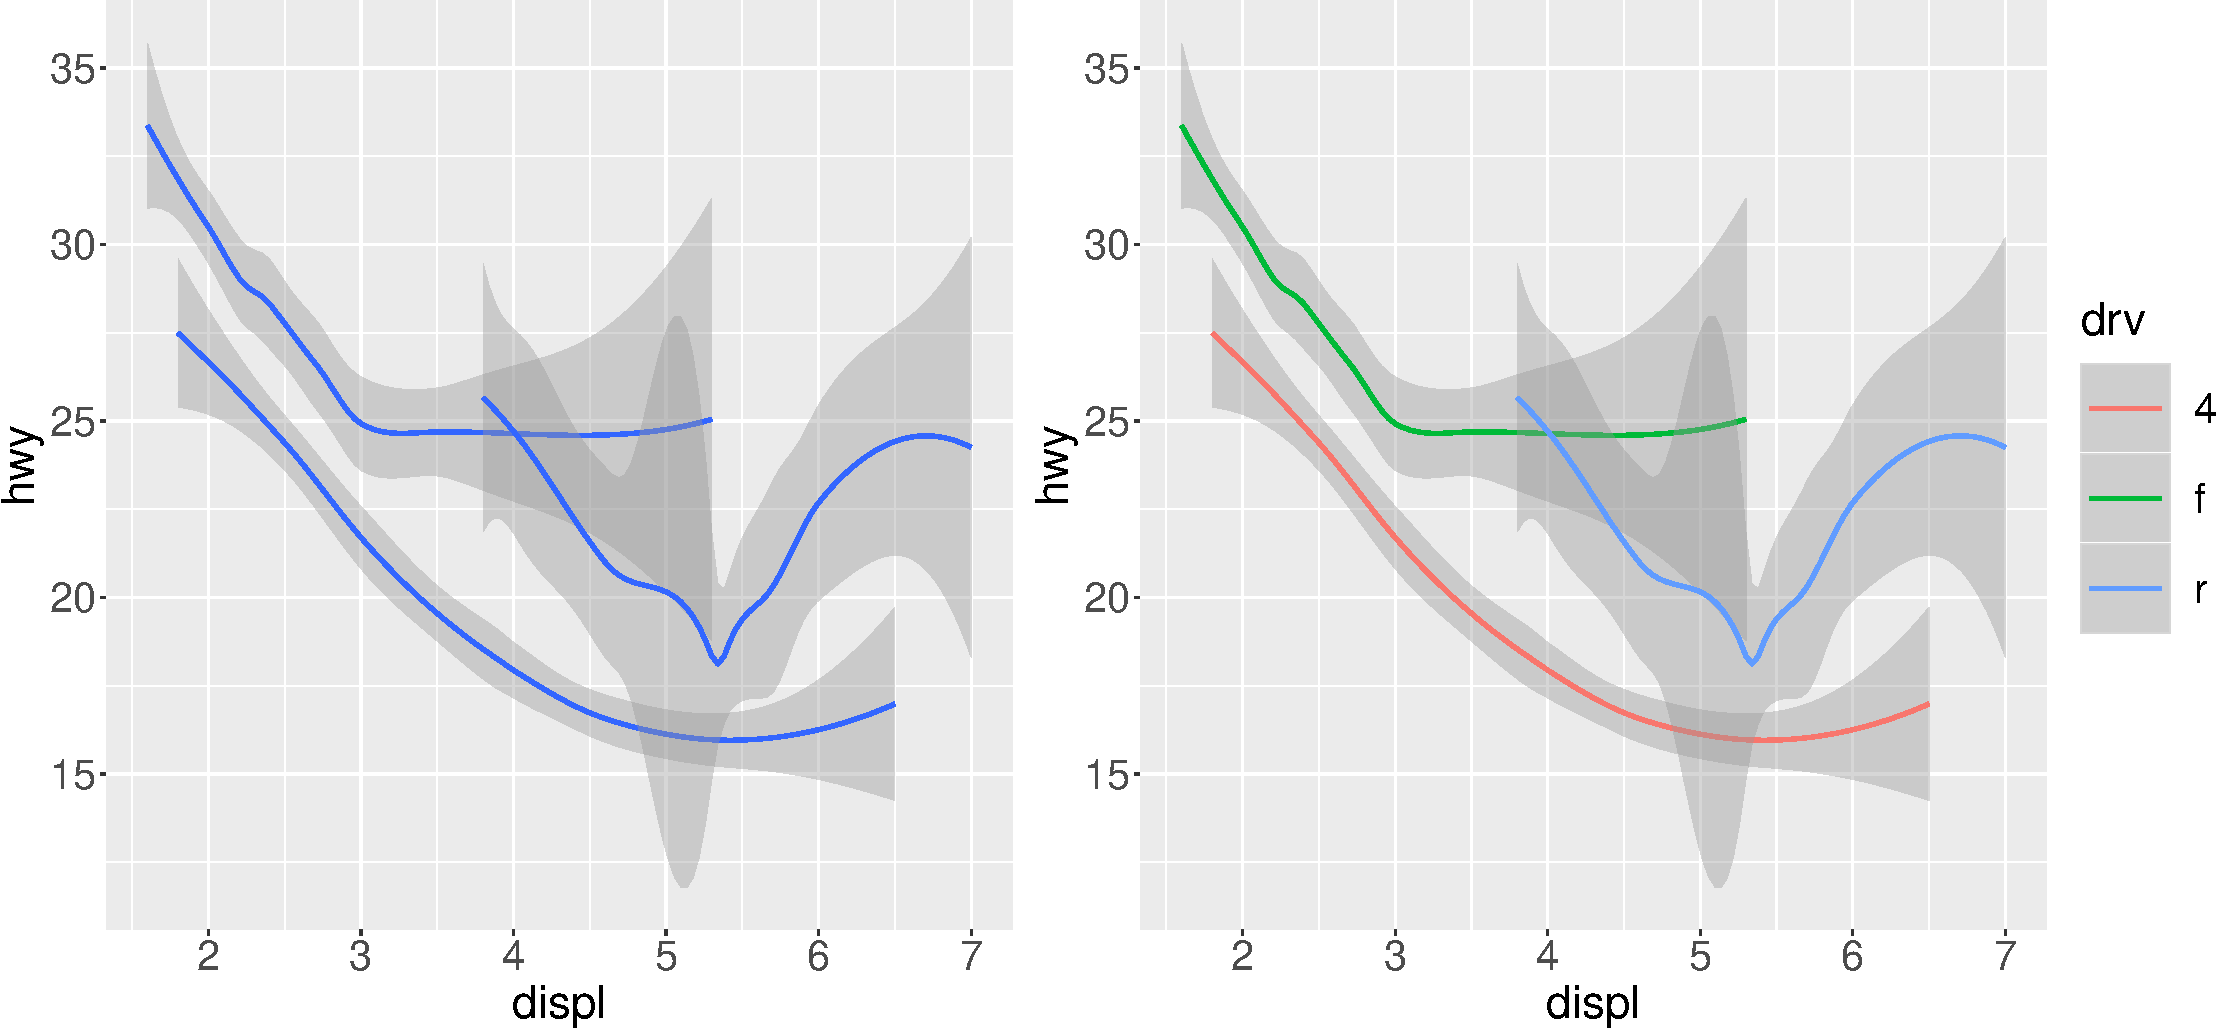
\includegraphics[height=150px]{data-visualization_files/figure-beamer/unnamed-chunk-35-1} \end{center}

\end{frame}

\begin{frame}[fragile]{Aesthetics and logical conditions}
\protect\hypertarget{aesthetics-and-logical-conditions}{}

Aesthetics can be mapped to logical expressions. For example, if you map
an aesthetic to \texttt{displ\ \textless{}\ 5}:

\begin{itemize}
\item
  \texttt{ggplot()} creates a temporary variable with values equal to
  the result \texttt{displ\ \textless{}\ 5}.
\item
  The result of \texttt{displ\ \textless{}\ 5} is a logical variable.
\item
  \texttt{ggplot()} then maps the aesthetic to the temporary variable.
\end{itemize}

\end{frame}

\begin{frame}[fragile]{Aesthetics and logical conditions}
\protect\hypertarget{aesthetics-and-logical-conditions-1}{}

\begin{Shaded}
\begin{Highlighting}[]
\KeywordTok{ggplot}\NormalTok{(mpg) }\OperatorTok{+}\StringTok{ }
\StringTok{  }\KeywordTok{geom_point}\NormalTok{(}\KeywordTok{aes}\NormalTok{(}\DataTypeTok{x =}\NormalTok{ displ, }\DataTypeTok{y =}\NormalTok{ hwy, }
                 \DataTypeTok{colour =}\NormalTok{ displ }\OperatorTok{<}\StringTok{ }\DecValTok{5}\NormalTok{))}
\end{Highlighting}
\end{Shaded}

\begin{center}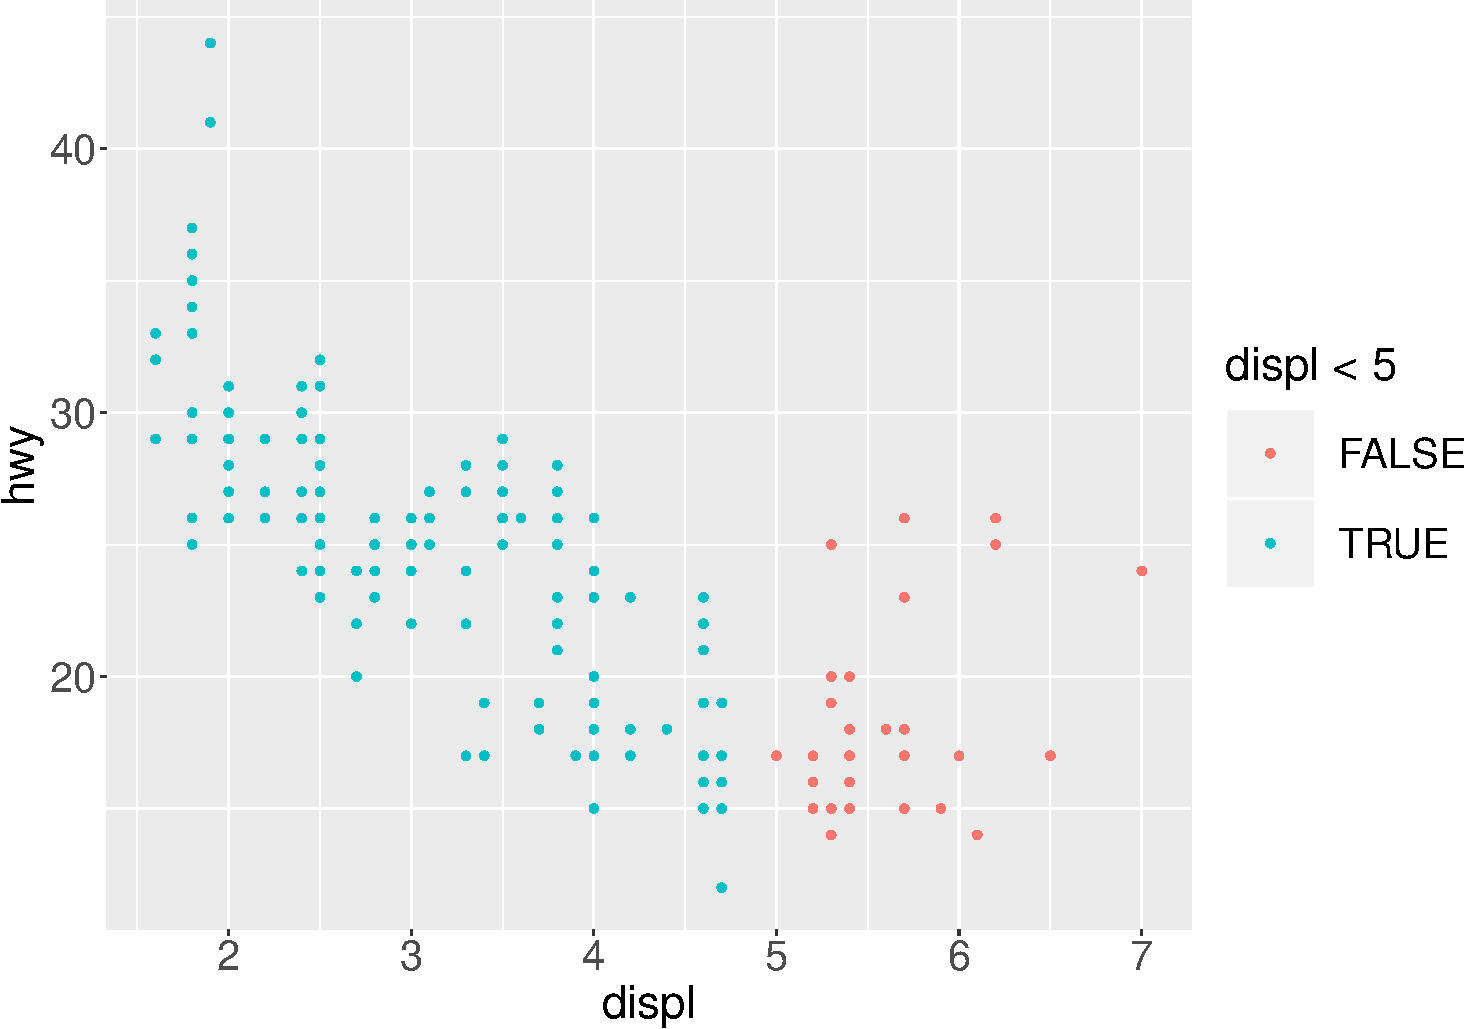
\includegraphics[height=150px]{data-visualization_files/figure-beamer/unnamed-chunk-36-1} \end{center}

\end{frame}

\begin{frame}[fragile]{Aesthetics and logical conditions}
\protect\hypertarget{aesthetics-and-logical-conditions-2}{}

\begin{Shaded}
\begin{Highlighting}[]
\KeywordTok{ggplot}\NormalTok{(mpg) }\OperatorTok{+}\StringTok{ }
\StringTok{  }\KeywordTok{geom_point}\NormalTok{(}\KeywordTok{aes}\NormalTok{(}\DataTypeTok{x =}\NormalTok{ displ, }\DataTypeTok{y =}\NormalTok{ hwy, }
                 \DataTypeTok{colour =}\NormalTok{ class }\OperatorTok{==}\StringTok{ "2seater"}\NormalTok{))}
\end{Highlighting}
\end{Shaded}

\begin{center}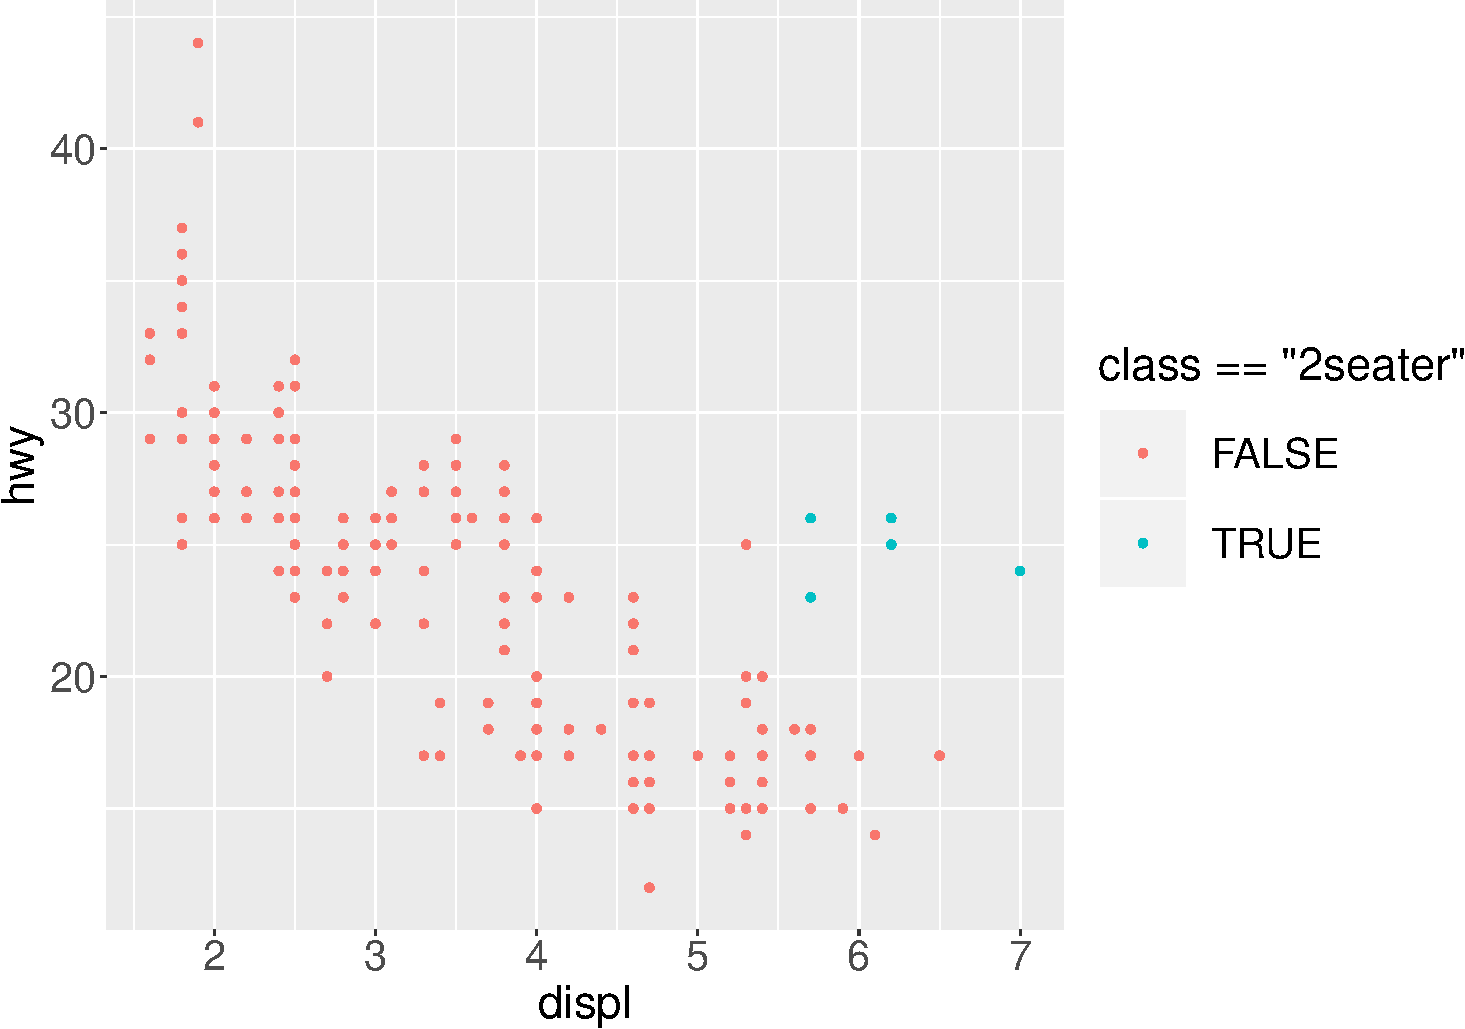
\includegraphics[height=150px]{data-visualization_files/figure-beamer/unnamed-chunk-37-1} \end{center}

\end{frame}

\begin{frame}{Changing default aesthetic properties of geoms}
\protect\hypertarget{changing-default-aesthetic-properties-of-geoms}{}

\begin{itemize}
\item
  To change a default aesthetic property, set the aesthetic by name as
  an argument of the geom function.

  \begin{itemize}
  \item
    Names of colors should be indicated as character strings.
  \item
    Size of points should be indicated in mm.
  \item
    Shapes are identified by the numbers in figure 3.
  \end{itemize}
\end{itemize}

\end{frame}

\begin{frame}[fragile]{Changing default aesthetic properties of geoms}
\protect\hypertarget{changing-default-aesthetic-properties-of-geoms-1}{}

\begin{itemize}
\item
  There are some seeming duplicate shapes (e.g.~0, 15, and 22 are all
  squares).
\item
  The difference comes from the interaction of the \texttt{colour} and
  \texttt{fill} aesthetics:

  \begin{itemize}
  \item
    The hollow shapes (0--14) have a border determined by the
    \texttt{colour} aesthetic
  \item
    The solid shapes (15--18) are filled with the colour
    \texttt{aesthetic}
  \item
    The filled shapes (21--24) have a border set by the \texttt{colour}
    aesthetic and are filled with the \texttt{fill} aesthetic
  \end{itemize}
\end{itemize}

\end{frame}

\begin{frame}[fragile]{Changing default aesthetic properties of geoms}
\protect\hypertarget{changing-default-aesthetic-properties-of-geoms-2}{}

For example, we can make all of the points blue:

\begin{Shaded}
\begin{Highlighting}[]
\KeywordTok{ggplot}\NormalTok{(}\DataTypeTok{data =}\NormalTok{ mpg) }\OperatorTok{+}
\StringTok{  }\KeywordTok{geom_point}\NormalTok{(}\KeywordTok{aes}\NormalTok{(}\DataTypeTok{x =}\NormalTok{ displ, }\DataTypeTok{y =}\NormalTok{ hwy), }
    \DataTypeTok{color =} \StringTok{"blue"}\NormalTok{)}
\end{Highlighting}
\end{Shaded}

\end{frame}

\begin{frame}{Changing default aesthetic properties of geoms}
\protect\hypertarget{changing-default-aesthetic-properties-of-geoms-3}{}

\begin{center}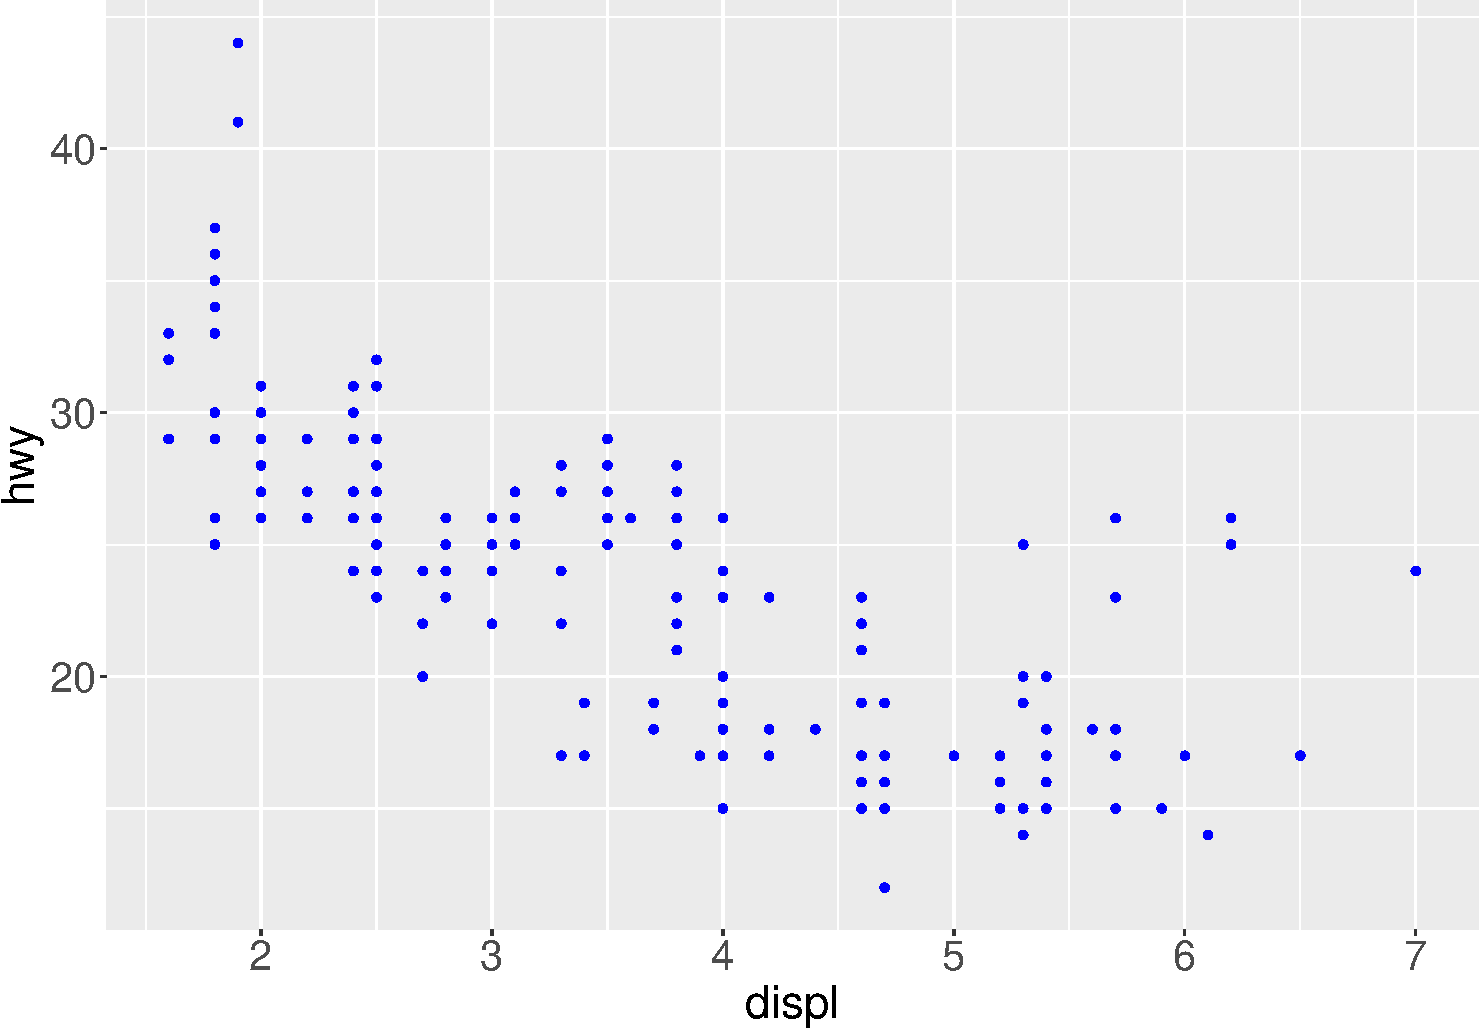
\includegraphics[height=200px]{data-visualization_files/figure-beamer/unnamed-chunk-39-1} \end{center}

\end{frame}

\begin{frame}[fragile]{Changing default aesthetic properties of geoms}
\protect\hypertarget{changing-default-aesthetic-properties-of-geoms-4}{}

Now let's change the size of the points:

\begin{Shaded}
\begin{Highlighting}[]
\KeywordTok{ggplot}\NormalTok{(}\DataTypeTok{data =}\NormalTok{ mpg) }\OperatorTok{+}
\StringTok{  }\KeywordTok{geom_point}\NormalTok{(}\KeywordTok{aes}\NormalTok{(}\DataTypeTok{x =}\NormalTok{ displ, }\DataTypeTok{y =}\NormalTok{ hwy), }
    \DataTypeTok{color =} \StringTok{"blue"}\NormalTok{,}
    \DataTypeTok{size =} \DecValTok{6}\NormalTok{)}
\end{Highlighting}
\end{Shaded}

\end{frame}

\begin{frame}{Changing default aesthetic properties of geoms}
\protect\hypertarget{changing-default-aesthetic-properties-of-geoms-5}{}

\begin{center}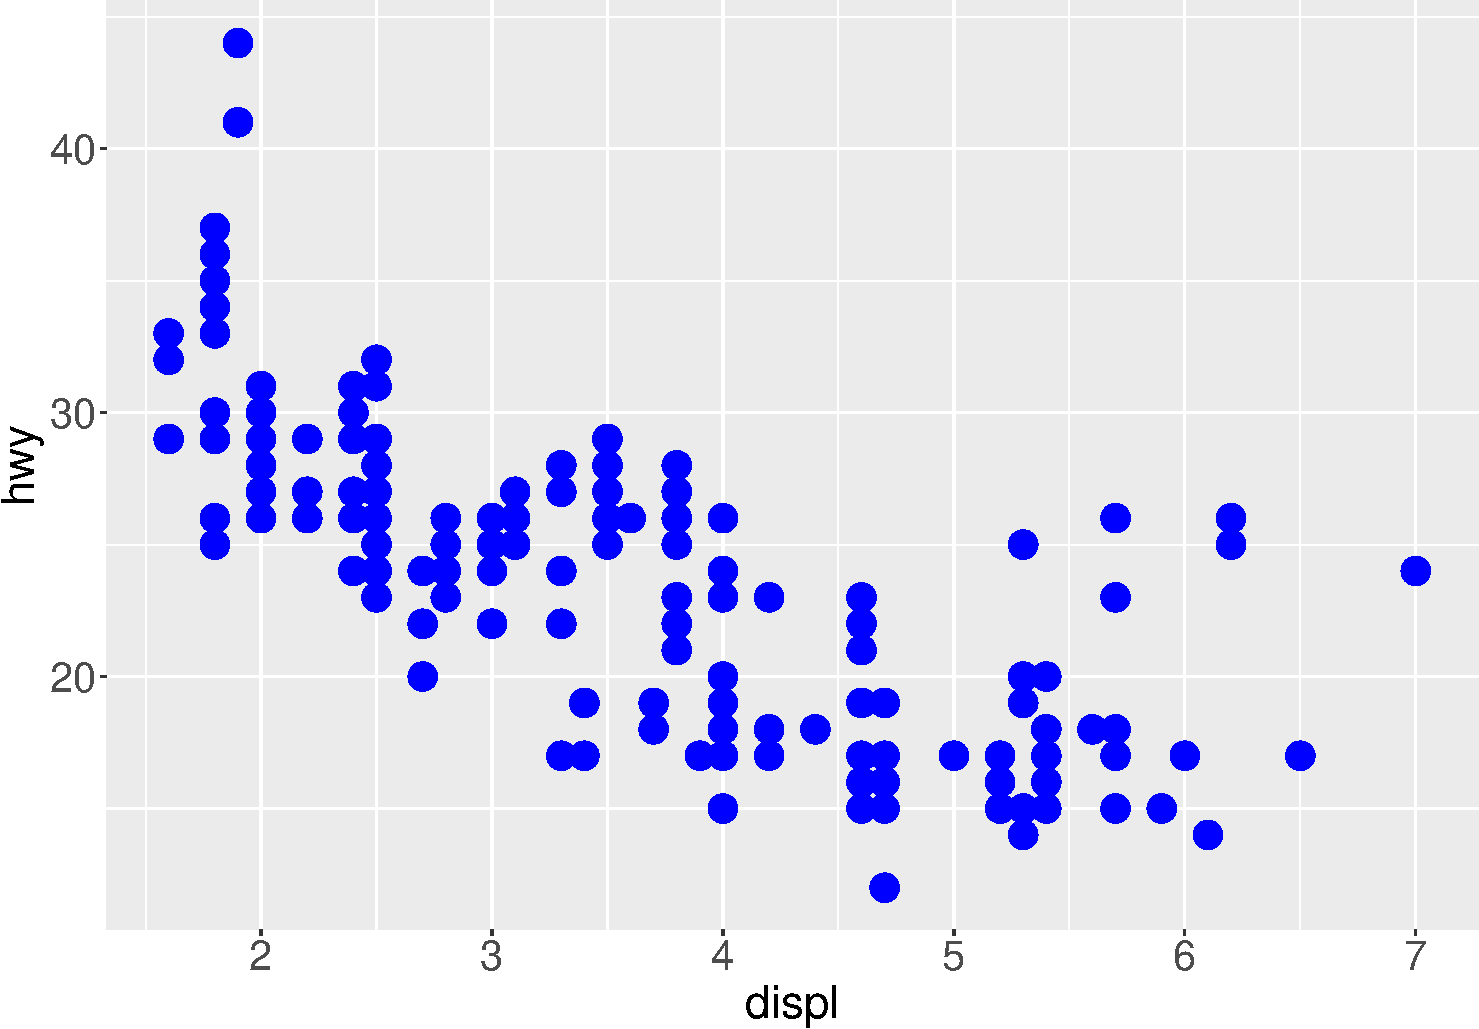
\includegraphics[height=200px]{data-visualization_files/figure-beamer/unnamed-chunk-41-1} \end{center}

\end{frame}

\begin{frame}[fragile]{Changing default aesthetic properties of geoms}
\protect\hypertarget{changing-default-aesthetic-properties-of-geoms-6}{}

We can also change the default shape of the points:

\begin{Shaded}
\begin{Highlighting}[]
\KeywordTok{ggplot}\NormalTok{(}\DataTypeTok{data =}\NormalTok{ mpg) }\OperatorTok{+}\StringTok{ }
\StringTok{  }\KeywordTok{geom_point}\NormalTok{(}\KeywordTok{aes}\NormalTok{(}\DataTypeTok{x =}\NormalTok{ displ, }\DataTypeTok{y =}\NormalTok{ hwy), }
    \DataTypeTok{color =} \StringTok{"blue"}\NormalTok{,}
    \DataTypeTok{size =} \DecValTok{5}\NormalTok{,}
    \DataTypeTok{shape =} \DecValTok{6}\NormalTok{)}
\end{Highlighting}
\end{Shaded}

\end{frame}

\begin{frame}{Changing default aesthetic properties of geoms}
\protect\hypertarget{changing-default-aesthetic-properties-of-geoms-7}{}

\begin{center}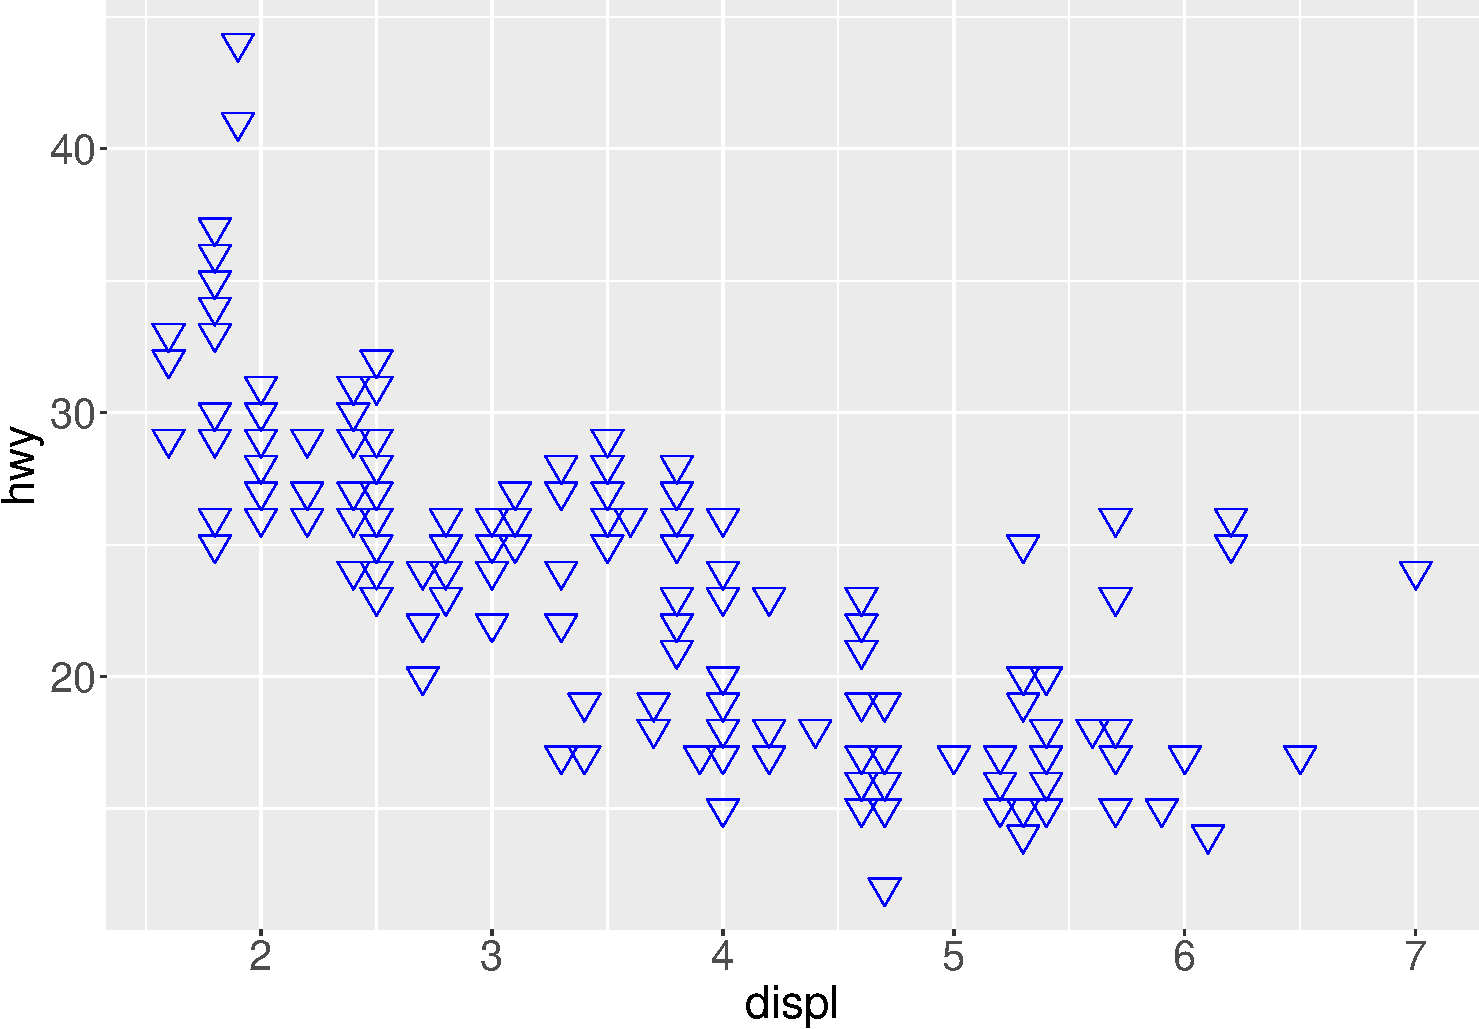
\includegraphics[height=200px]{data-visualization_files/figure-beamer/unnamed-chunk-43-1} \end{center}

\end{frame}

\begin{frame}[fragile]{Changing default aesthetic properties of geoms}
\protect\hypertarget{changing-default-aesthetic-properties-of-geoms-8}{}

\begin{itemize}
\item
  Shape 6 is a hollow shape, it interacts only with the \texttt{color}
  aesthetic.
\item
  If we want triangles filled with color, we must use shape 24, which
  interacts both with the color and \texttt{fill} aesthetics:
\end{itemize}

\begin{Shaded}
\begin{Highlighting}[]
\KeywordTok{ggplot}\NormalTok{(}\DataTypeTok{data =}\NormalTok{ mpg) }\OperatorTok{+}
\StringTok{  }\KeywordTok{geom_point}\NormalTok{(}
    \DataTypeTok{mapping =} \KeywordTok{aes}\NormalTok{(}\DataTypeTok{x =}\NormalTok{ displ, }\DataTypeTok{y =}\NormalTok{ hwy),}
    \DataTypeTok{color =} \StringTok{"blue"}\NormalTok{,}
    \DataTypeTok{size =} \DecValTok{5}\NormalTok{,}
    \DataTypeTok{shape =} \DecValTok{24}\NormalTok{,}
    \DataTypeTok{fill =} \StringTok{"red"}
\NormalTok{  )}
\end{Highlighting}
\end{Shaded}

\end{frame}

\begin{frame}{Changing default aesthetic properties of geoms}
\protect\hypertarget{changing-default-aesthetic-properties-of-geoms-9}{}

\begin{center}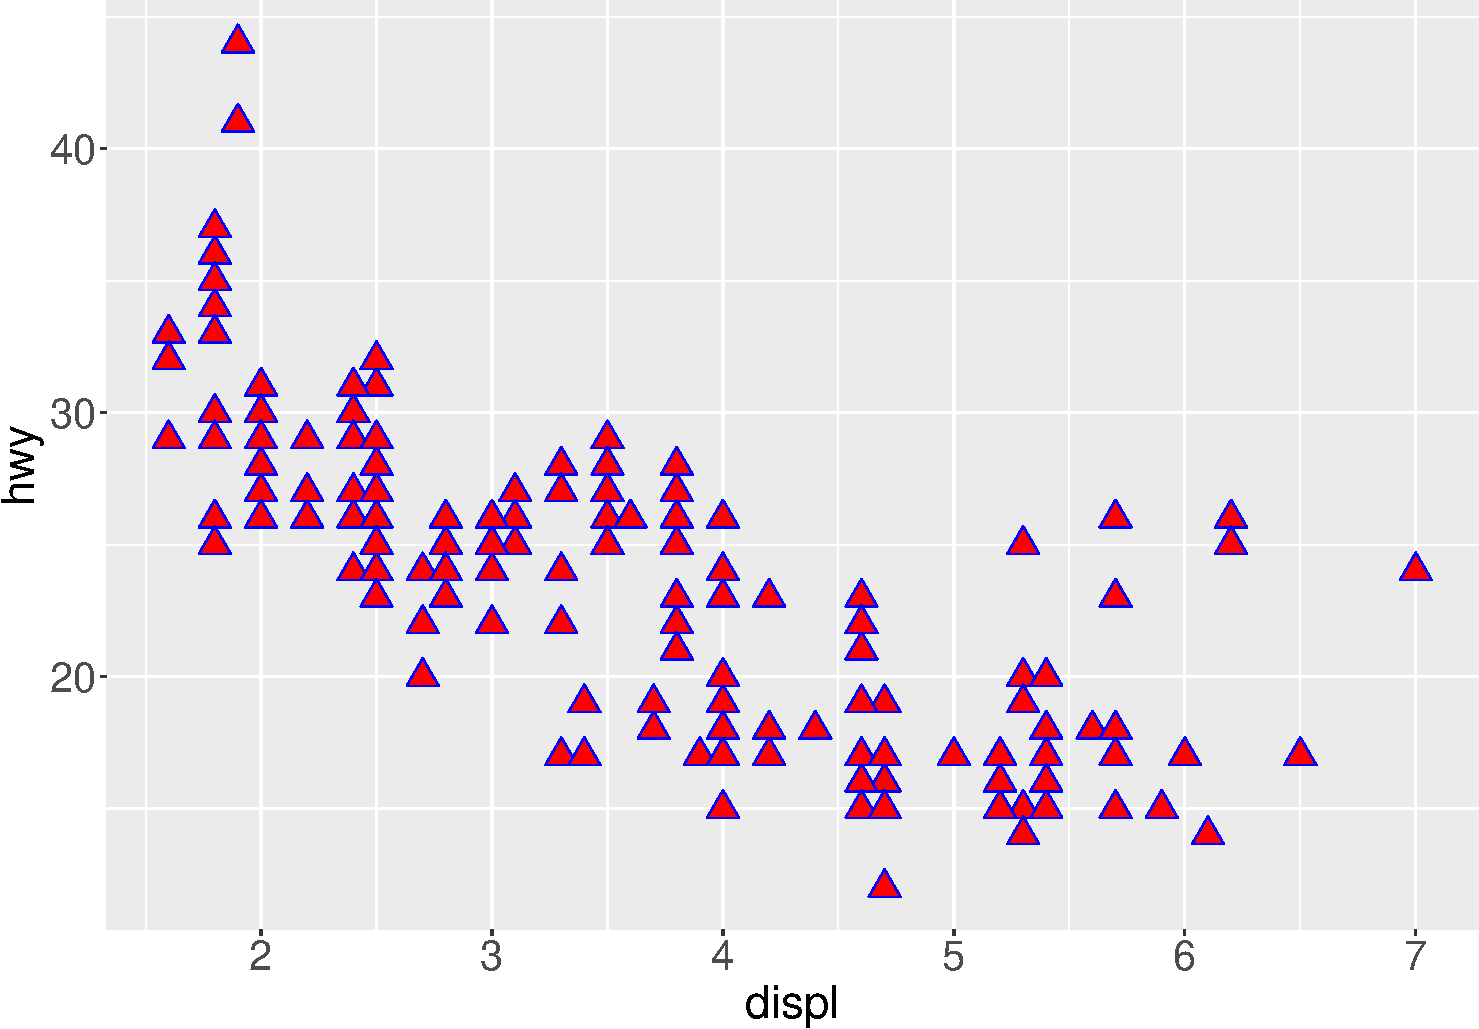
\includegraphics[height=200px]{data-visualization_files/figure-beamer/unnamed-chunk-45-1} \end{center}

\end{frame}

\begin{frame}[fragile]{Changing default aesthetic properties of geoms}
\protect\hypertarget{changing-default-aesthetic-properties-of-geoms-10}{}

The \texttt{stroke} aesthetic changes the thickness of the border of the
points:

\begin{Shaded}
\begin{Highlighting}[]
\KeywordTok{ggplot}\NormalTok{(}\DataTypeTok{data =}\NormalTok{ mpg) }\OperatorTok{+}
\StringTok{  }\KeywordTok{geom_point}\NormalTok{(}\KeywordTok{aes}\NormalTok{(}\DataTypeTok{x =}\NormalTok{ displ, }\DataTypeTok{y =}\NormalTok{ hwy),}
    \DataTypeTok{color =} \StringTok{"blue"}\NormalTok{,}
    \DataTypeTok{size =} \DecValTok{5}\NormalTok{,}
    \DataTypeTok{shape =} \DecValTok{23}\NormalTok{,}
    \DataTypeTok{fill =} \StringTok{"red"}\NormalTok{,}
    \DataTypeTok{stroke =} \DecValTok{2}
\NormalTok{  )}
\end{Highlighting}
\end{Shaded}

\end{frame}

\begin{frame}{Changing default aesthetic properties of geoms}
\protect\hypertarget{changing-default-aesthetic-properties-of-geoms-11}{}

\begin{center}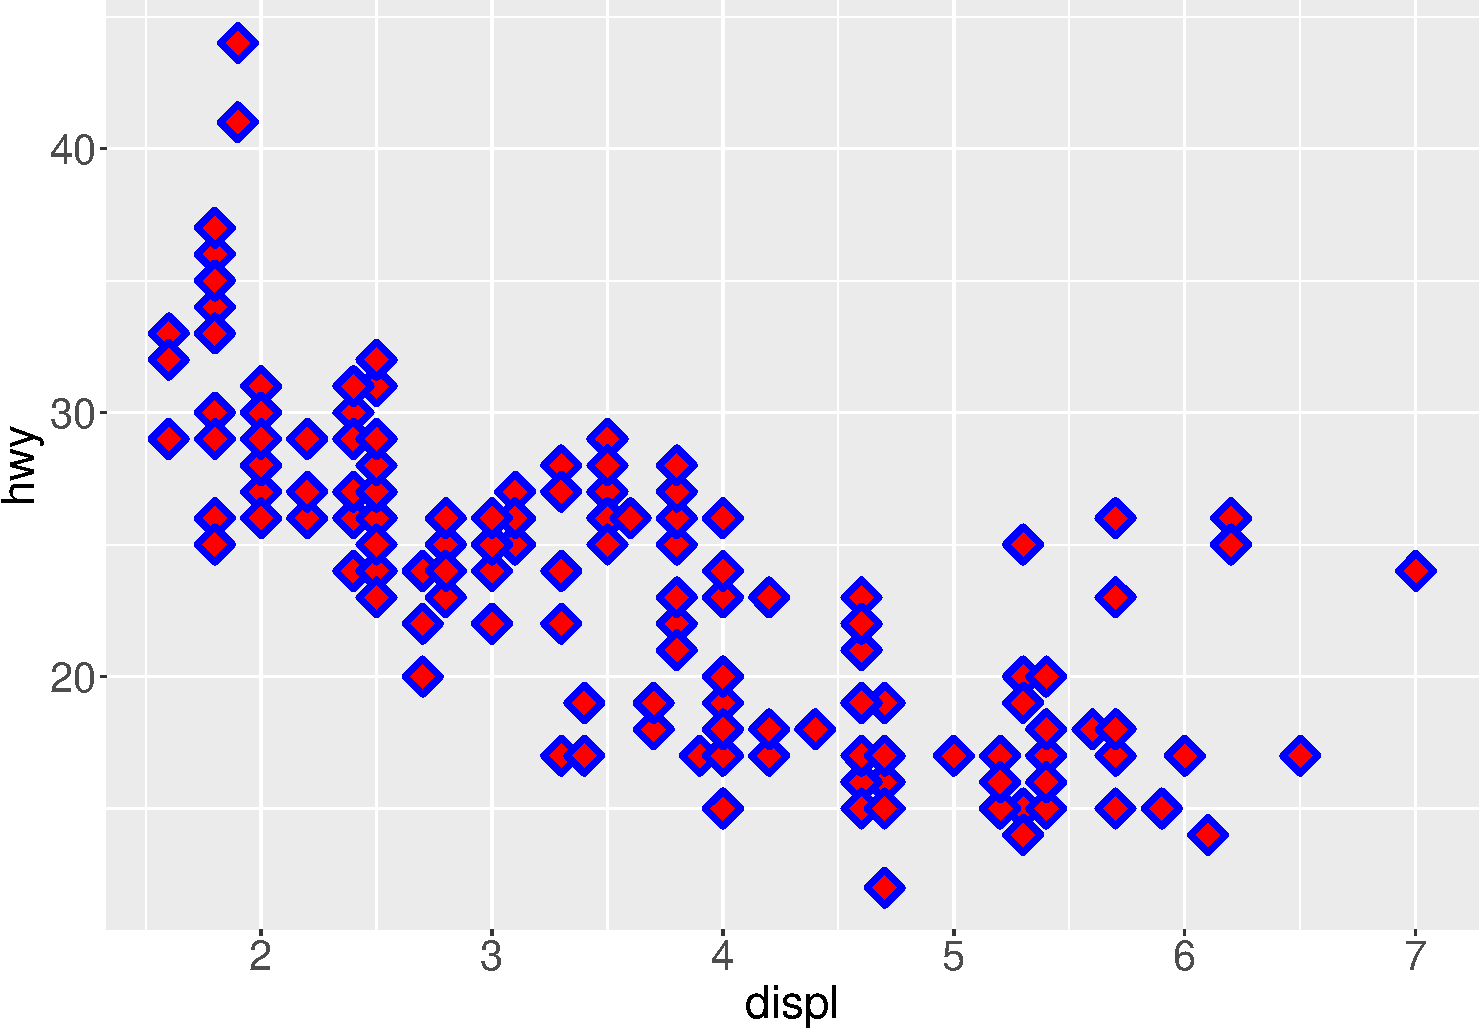
\includegraphics[height=200px]{data-visualization_files/figure-beamer/unnamed-chunk-47-1} \end{center}

\end{frame}

\begin{frame}[fragile]{Changing default aesthetic properties of geoms}
\protect\hypertarget{changing-default-aesthetic-properties-of-geoms-12}{}

You can also use colors like dark blue and light blue:

\begin{Shaded}
\begin{Highlighting}[]
\KeywordTok{ggplot}\NormalTok{(}\DataTypeTok{data =}\NormalTok{ mpg) }\OperatorTok{+}
\StringTok{  }\KeywordTok{geom_point}\NormalTok{(}\KeywordTok{aes}\NormalTok{(}\DataTypeTok{x =}\NormalTok{ displ, }\DataTypeTok{y =}\NormalTok{ hwy),}
    \DataTypeTok{color =} \StringTok{"darkblue"}\NormalTok{,}
    \DataTypeTok{fill =} \StringTok{"lightblue"}\NormalTok{,}
    \DataTypeTok{shape =} \DecValTok{21}\NormalTok{,}
    \DataTypeTok{size =} \DecValTok{5}\NormalTok{,}
    \DataTypeTok{stroke =} \DecValTok{1}
\NormalTok{  )}
\end{Highlighting}
\end{Shaded}

\end{frame}

\begin{frame}{Changing default aesthetic properties of geoms}
\protect\hypertarget{changing-default-aesthetic-properties-of-geoms-13}{}

\begin{center}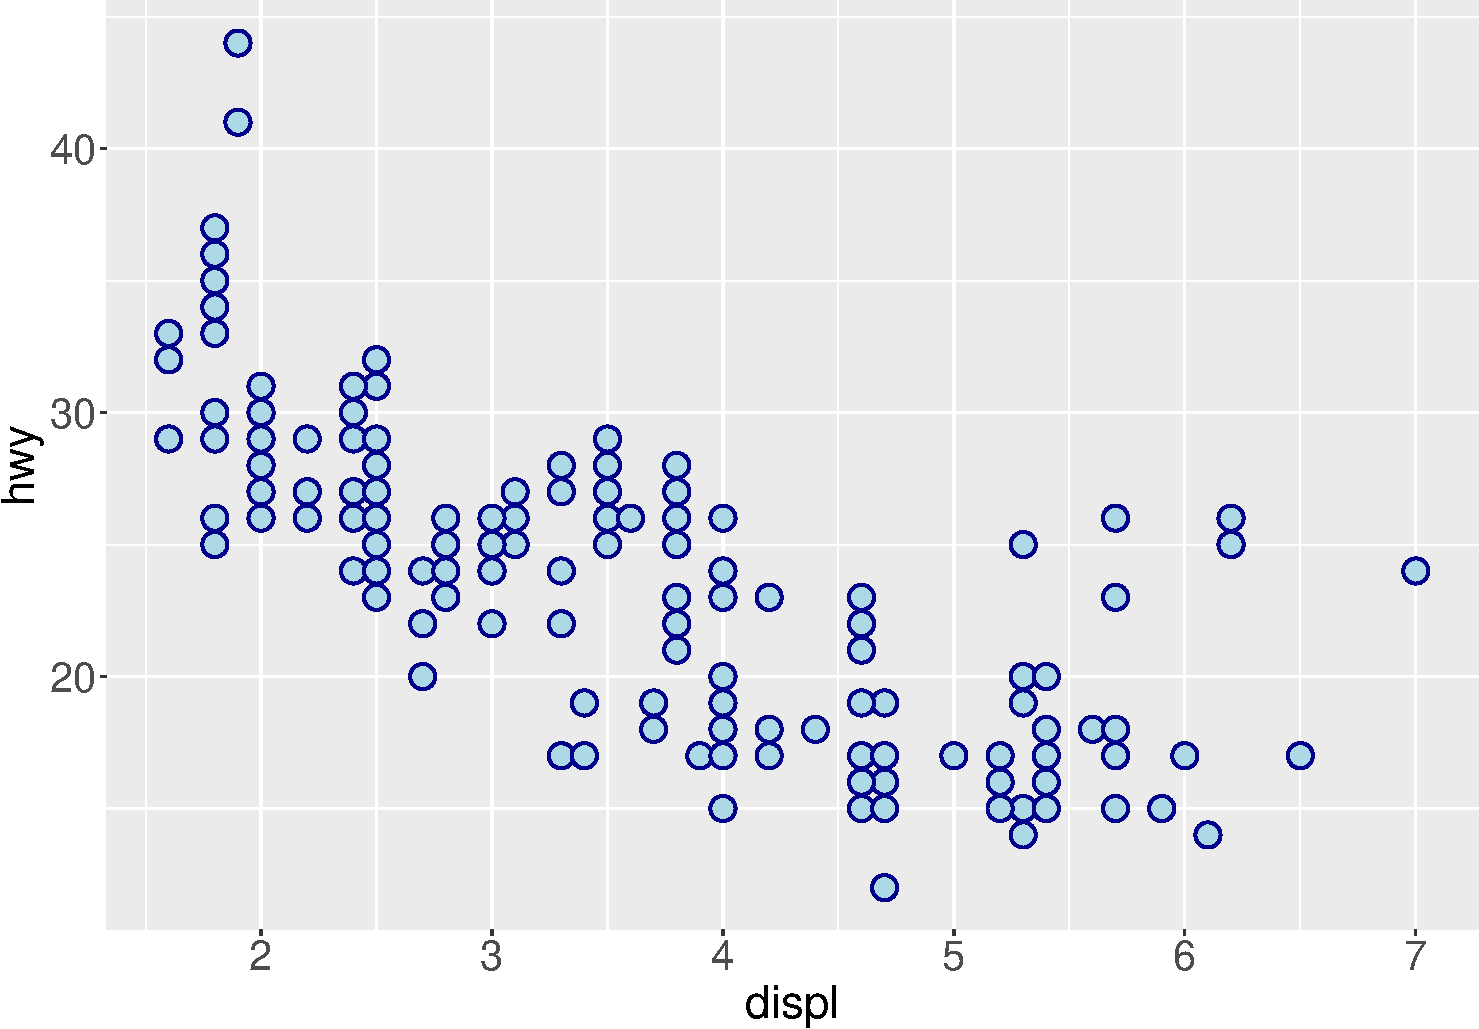
\includegraphics[height=200px]{data-visualization_files/figure-beamer/unnamed-chunk-49-1} \end{center}

\end{frame}

\begin{frame}[fragile]{Changing default aesthetic properties of geoms}
\protect\hypertarget{changing-default-aesthetic-properties-of-geoms-14}{}

\begin{Shaded}
\begin{Highlighting}[]
\KeywordTok{ggplot}\NormalTok{(}\DataTypeTok{data =}\NormalTok{ mpg) }\OperatorTok{+}
\StringTok{  }\KeywordTok{geom_point}\NormalTok{(}\KeywordTok{aes}\NormalTok{(}\DataTypeTok{x =}\NormalTok{ displ, }\DataTypeTok{y =}\NormalTok{ hwy),}
    \DataTypeTok{color =} \StringTok{"darkblue"}\NormalTok{,}
    \DataTypeTok{fill =} \StringTok{"lightblue"}\NormalTok{,}
    \DataTypeTok{shape =} \DecValTok{21}\NormalTok{,}
    \DataTypeTok{size =} \DecValTok{5}\NormalTok{,}
    \DataTypeTok{stroke =} \DecValTok{3}
\NormalTok{  )}
\end{Highlighting}
\end{Shaded}

\end{frame}

\begin{frame}{Changing default aesthetic properties of geoms}
\protect\hypertarget{changing-default-aesthetic-properties-of-geoms-15}{}

\begin{center}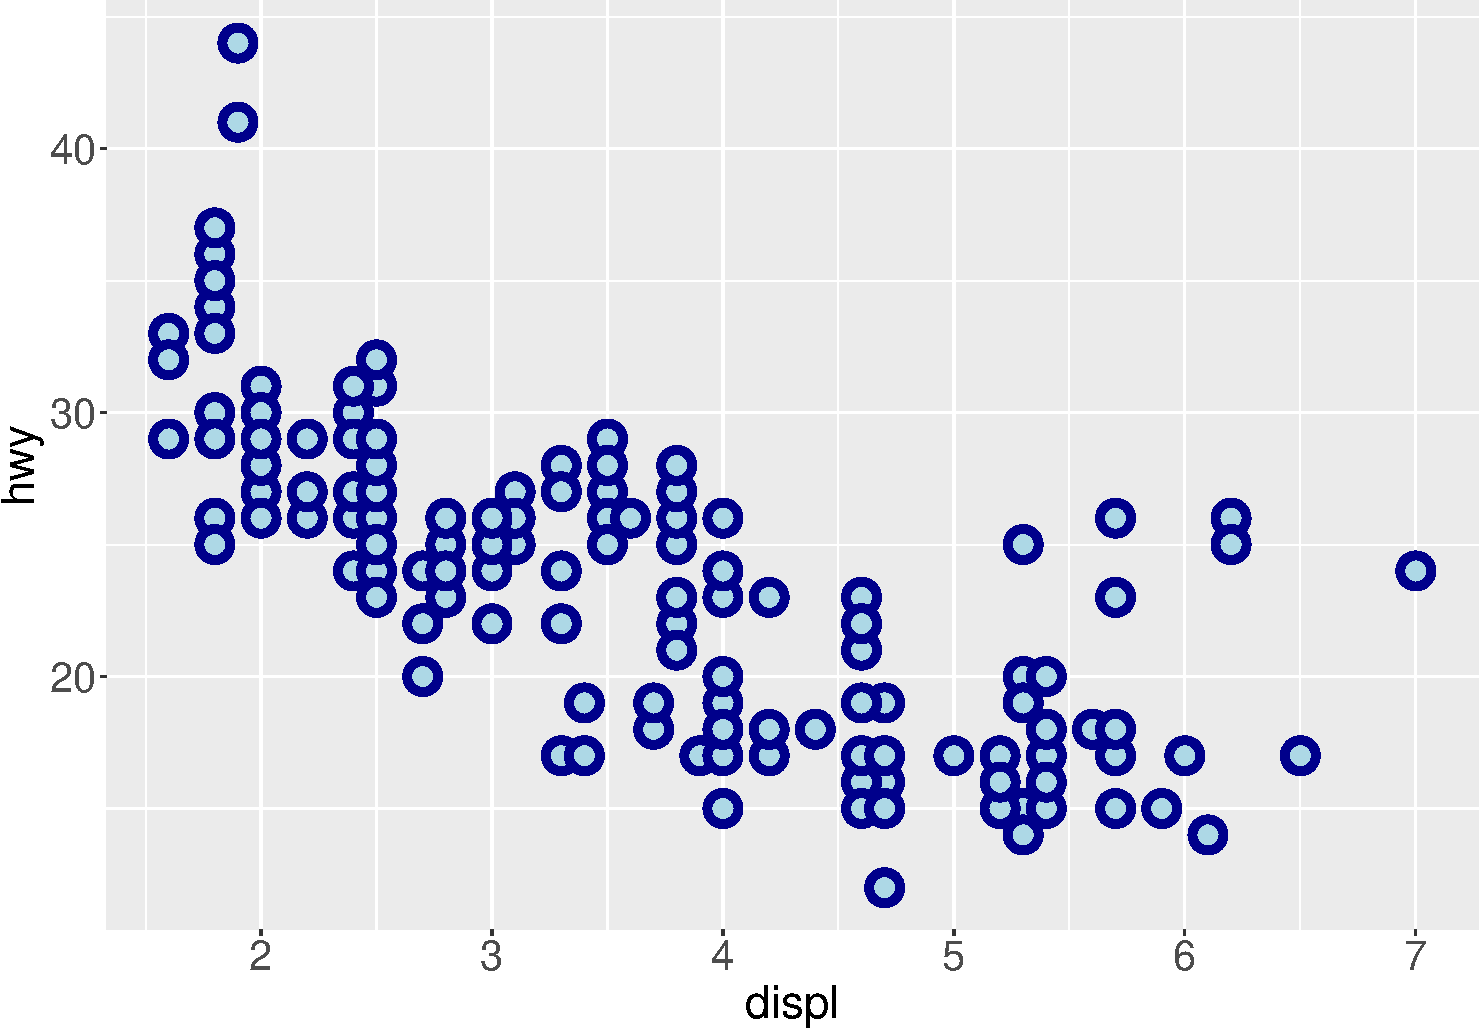
\includegraphics[height=200px]{data-visualization_files/figure-beamer/unnamed-chunk-51-1} \end{center}

\end{frame}

\begin{frame}{Changing default aesthetic properties of geoms}
\protect\hypertarget{changing-default-aesthetic-properties-of-geoms-16}{}

\begin{itemize}
\tightlist
\item
  For a list of available colors and their names see:
  \url{http://sape.inf.usi.ch/quick-reference/ggplot2/colour}
\end{itemize}

\end{frame}

\begin{frame}{Changing default aesthetic properties of geoms}
\protect\hypertarget{changing-default-aesthetic-properties-of-geoms-17}{}

\begin{itemize}
\item
  Alternatively, you can use RGB codes.
\item
  The RGB model reproduces a broad array of colors by mixing together
  red, green, and blue in different proportions.
\item
  You can specify colors like in HTML/CSS, using the hexadecimal values
  (00 to FF) for red, green, and blue, concatenated into a string,
  prefixed with a ``\#''.
\item
  A pure red colour this is represented with ``\#FF0000''.
\end{itemize}

See:

\begin{itemize}
\tightlist
\item
  \url{https://www.rapidtables.com/web/color/RGB_Color.html}
\item
  \url{https://htmlcolorcodes.com}
\end{itemize}

\end{frame}

\begin{frame}[fragile]{Changing default aesthetic properties of geoms}
\protect\hypertarget{changing-default-aesthetic-properties-of-geoms-18}{}

We can change the default line type of geom functions like
\texttt{geom\_smooth()}.

\begin{figure}
\centering
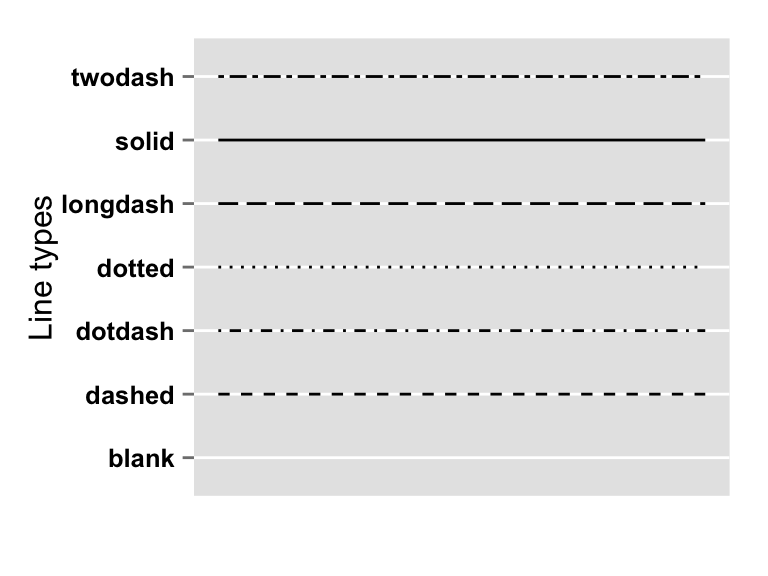
\includegraphics[width=2.60417in,height=\textheight]{figures/lty.png}
\caption{Built in line types}
\end{figure}

\end{frame}

\begin{frame}[fragile]{Changing default aesthetic properties of geoms}
\protect\hypertarget{changing-default-aesthetic-properties-of-geoms-19}{}

\begin{Shaded}
\begin{Highlighting}[]
\KeywordTok{ggplot}\NormalTok{(}\DataTypeTok{data =}\NormalTok{ mpg) }\OperatorTok{+}\StringTok{ }
\StringTok{  }\KeywordTok{geom_smooth}\NormalTok{(}\KeywordTok{aes}\NormalTok{(}\DataTypeTok{x =}\NormalTok{ displ, }\DataTypeTok{y =}\NormalTok{ hwy))}

\KeywordTok{ggplot}\NormalTok{(}\DataTypeTok{data =}\NormalTok{ mpg) }\OperatorTok{+}\StringTok{ }
\StringTok{  }\KeywordTok{geom_smooth}\NormalTok{(}\KeywordTok{aes}\NormalTok{(}\DataTypeTok{x =}\NormalTok{ displ, }\DataTypeTok{y =}\NormalTok{ hwy),}
    \DataTypeTok{linetype =} \StringTok{"dotted"}\NormalTok{)}

\KeywordTok{ggplot}\NormalTok{(}\DataTypeTok{data =}\NormalTok{ mpg) }\OperatorTok{+}\StringTok{ }
\StringTok{  }\KeywordTok{geom_smooth}\NormalTok{(}\KeywordTok{aes}\NormalTok{(}\DataTypeTok{x =}\NormalTok{ displ, }\DataTypeTok{y =}\NormalTok{ hwy),}
    \DataTypeTok{linetype =} \StringTok{"twodash"}\NormalTok{)}
\end{Highlighting}
\end{Shaded}

\end{frame}

\begin{frame}{Changing default aesthetic properties of geoms}
\protect\hypertarget{changing-default-aesthetic-properties-of-geoms-20}{}

\begin{center}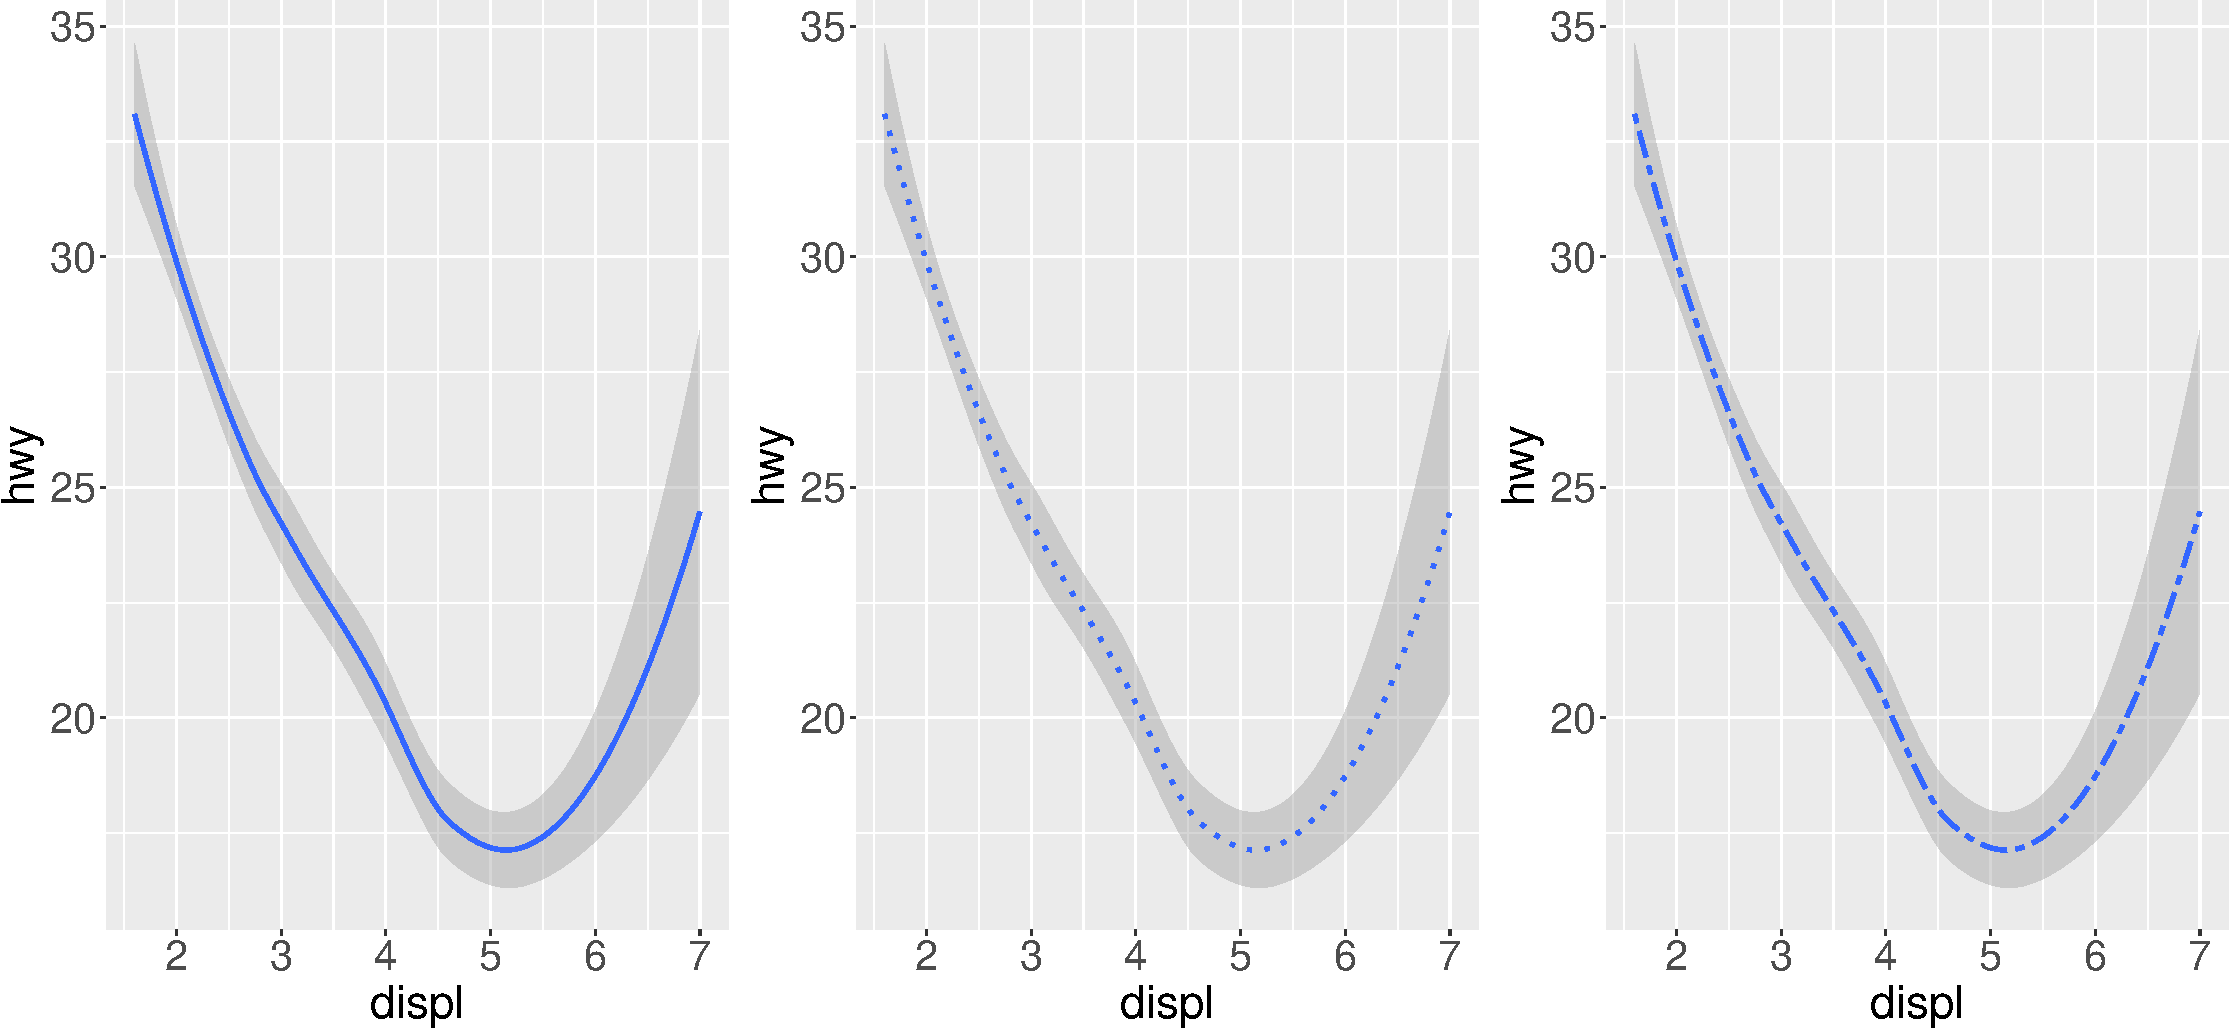
\includegraphics[height=150px]{data-visualization_files/figure-beamer/unnamed-chunk-53-1} \end{center}

\end{frame}

\begin{frame}[fragile]{Changing default aesthetic properties of geoms}
\protect\hypertarget{changing-default-aesthetic-properties-of-geoms-21}{}

We can also change the thickness of the lines:

\begin{Shaded}
\begin{Highlighting}[]
\KeywordTok{ggplot}\NormalTok{(}\DataTypeTok{data =}\NormalTok{ mpg) }\OperatorTok{+}\StringTok{ }
\StringTok{  }\KeywordTok{geom_smooth}\NormalTok{(}\KeywordTok{aes}\NormalTok{(}\DataTypeTok{x =}\NormalTok{ displ, }\DataTypeTok{y =}\NormalTok{ hwy))}

\KeywordTok{ggplot}\NormalTok{(}\DataTypeTok{data =}\NormalTok{ mpg) }\OperatorTok{+}\StringTok{ }
\StringTok{  }\KeywordTok{geom_smooth}\NormalTok{(}\KeywordTok{aes}\NormalTok{(}\DataTypeTok{x =}\NormalTok{ displ, }\DataTypeTok{y =}\NormalTok{ hwy), }\DataTypeTok{size =} \DecValTok{2}\NormalTok{)}

\KeywordTok{ggplot}\NormalTok{(}\DataTypeTok{data =}\NormalTok{ mpg) }\OperatorTok{+}\StringTok{ }
\StringTok{  }\KeywordTok{geom_smooth}\NormalTok{(}\KeywordTok{aes}\NormalTok{(}\DataTypeTok{x =}\NormalTok{ displ, }\DataTypeTok{y =}\NormalTok{ hwy), }\DataTypeTok{size =} \DecValTok{5}\NormalTok{)}
\end{Highlighting}
\end{Shaded}

\end{frame}

\begin{frame}{Changing default aesthetic properties of geoms}
\protect\hypertarget{changing-default-aesthetic-properties-of-geoms-22}{}

\begin{center}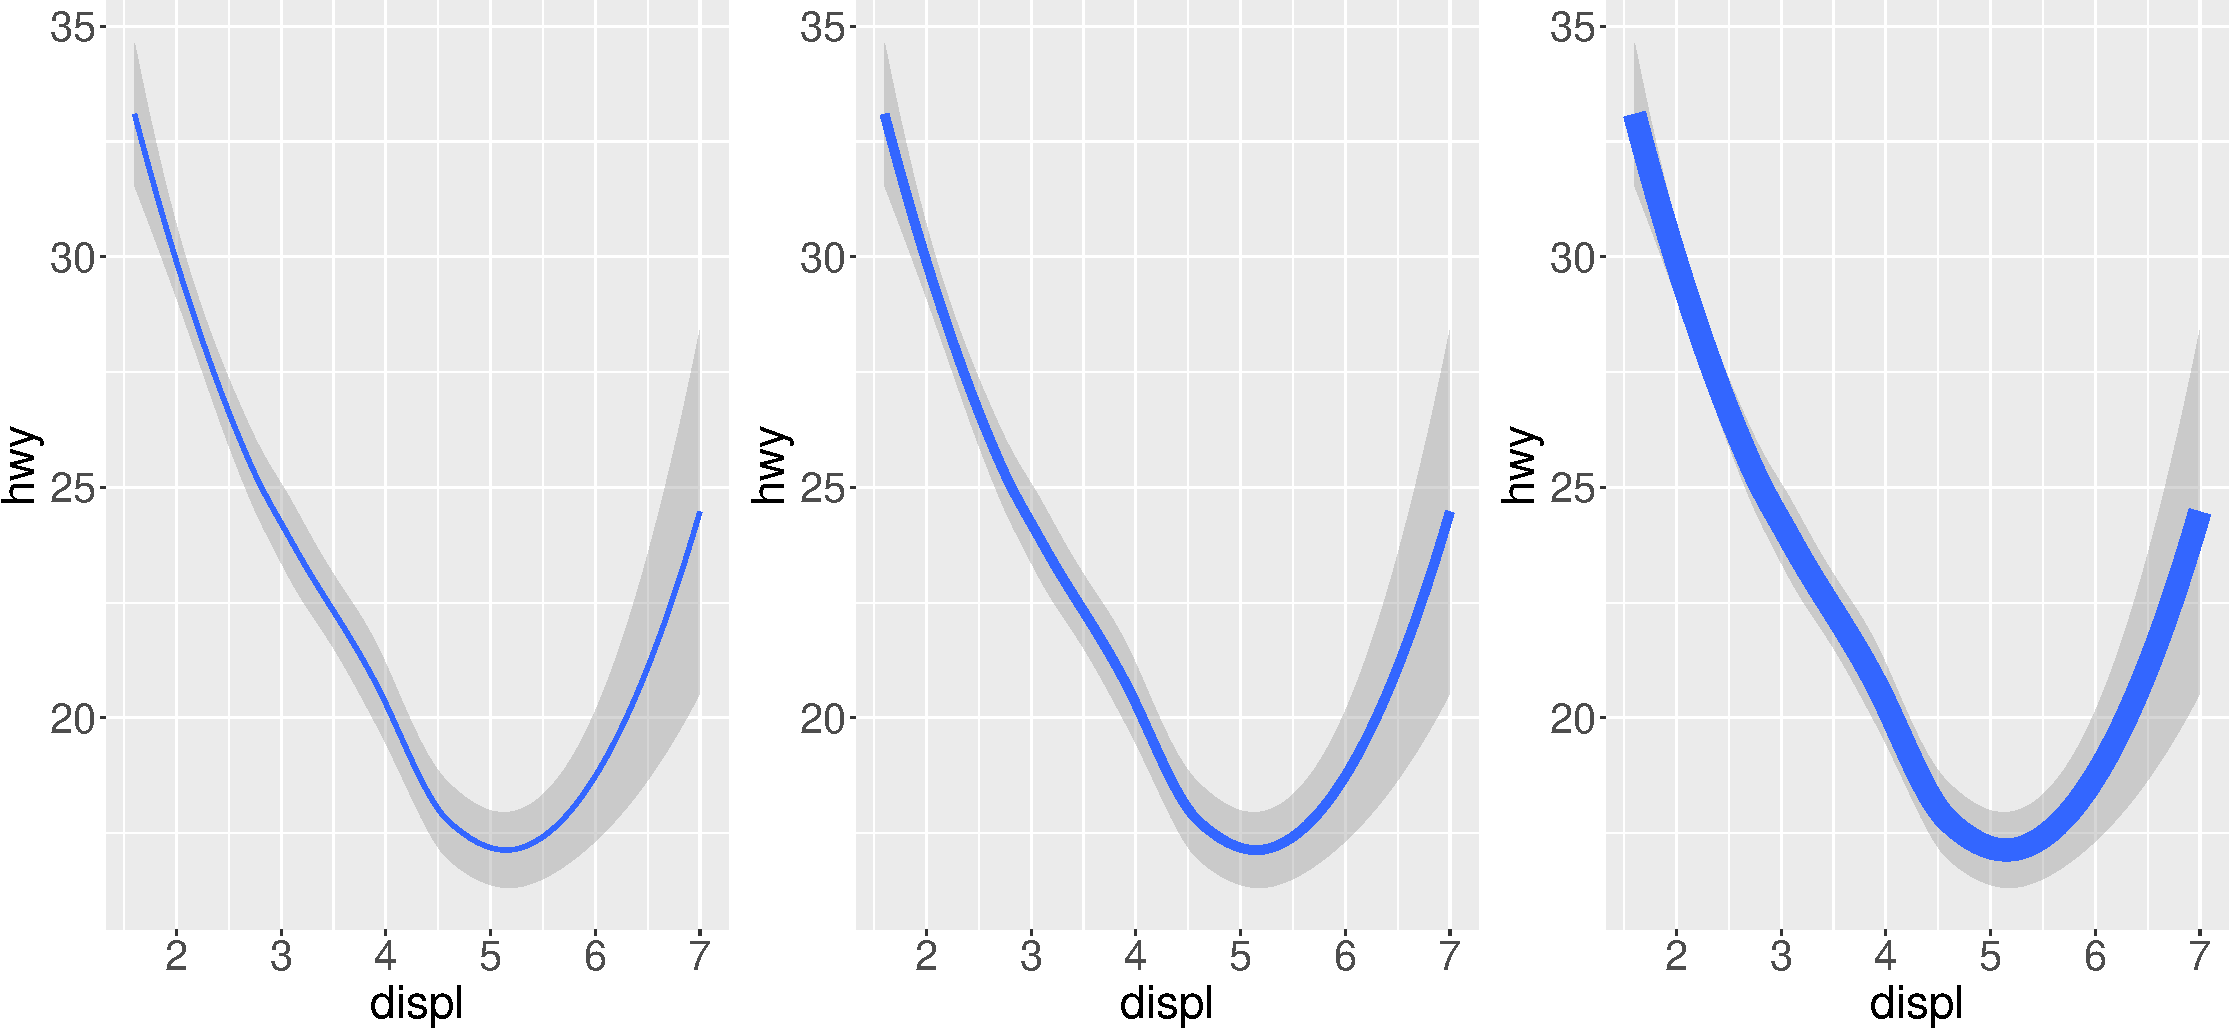
\includegraphics[height=150px]{data-visualization_files/figure-beamer/unnamed-chunk-55-1} \end{center}

\end{frame}

\begin{frame}[fragile]{Changing default aesthetic properties of geoms}
\protect\hypertarget{changing-default-aesthetic-properties-of-geoms-23}{}

\begin{Shaded}
\begin{Highlighting}[]
\KeywordTok{ggplot}\NormalTok{(}\DataTypeTok{data =}\NormalTok{ mpg) }\OperatorTok{+}\StringTok{ }
\StringTok{  }\KeywordTok{geom_smooth}\NormalTok{(}\KeywordTok{aes}\NormalTok{(}\DataTypeTok{x =}\NormalTok{ displ, }\DataTypeTok{y =}\NormalTok{ hwy),}
              \DataTypeTok{linetype =} \StringTok{"dotted"}\NormalTok{)}

\KeywordTok{ggplot}\NormalTok{(}\DataTypeTok{data =}\NormalTok{ mpg) }\OperatorTok{+}\StringTok{ }
\StringTok{  }\KeywordTok{geom_smooth}\NormalTok{(}\KeywordTok{aes}\NormalTok{(}\DataTypeTok{x =}\NormalTok{ displ, }\DataTypeTok{y =}\NormalTok{ hwy),}
              \DataTypeTok{linetype =} \StringTok{"dotted"}\NormalTok{, }\DataTypeTok{size =} \DecValTok{2}\NormalTok{)}

\KeywordTok{ggplot}\NormalTok{(}\DataTypeTok{data =}\NormalTok{ mpg) }\OperatorTok{+}\StringTok{ }
\StringTok{  }\KeywordTok{geom_smooth}\NormalTok{(}\KeywordTok{aes}\NormalTok{(}\DataTypeTok{x =}\NormalTok{ displ, }\DataTypeTok{y =}\NormalTok{ hwy),}
              \DataTypeTok{linetype =} \StringTok{"dotted"}\NormalTok{, }\DataTypeTok{size =} \DecValTok{5}\NormalTok{)}
\end{Highlighting}
\end{Shaded}

\end{frame}

\begin{frame}{Changing default aesthetic properties of geoms}
\protect\hypertarget{changing-default-aesthetic-properties-of-geoms-24}{}

\begin{center}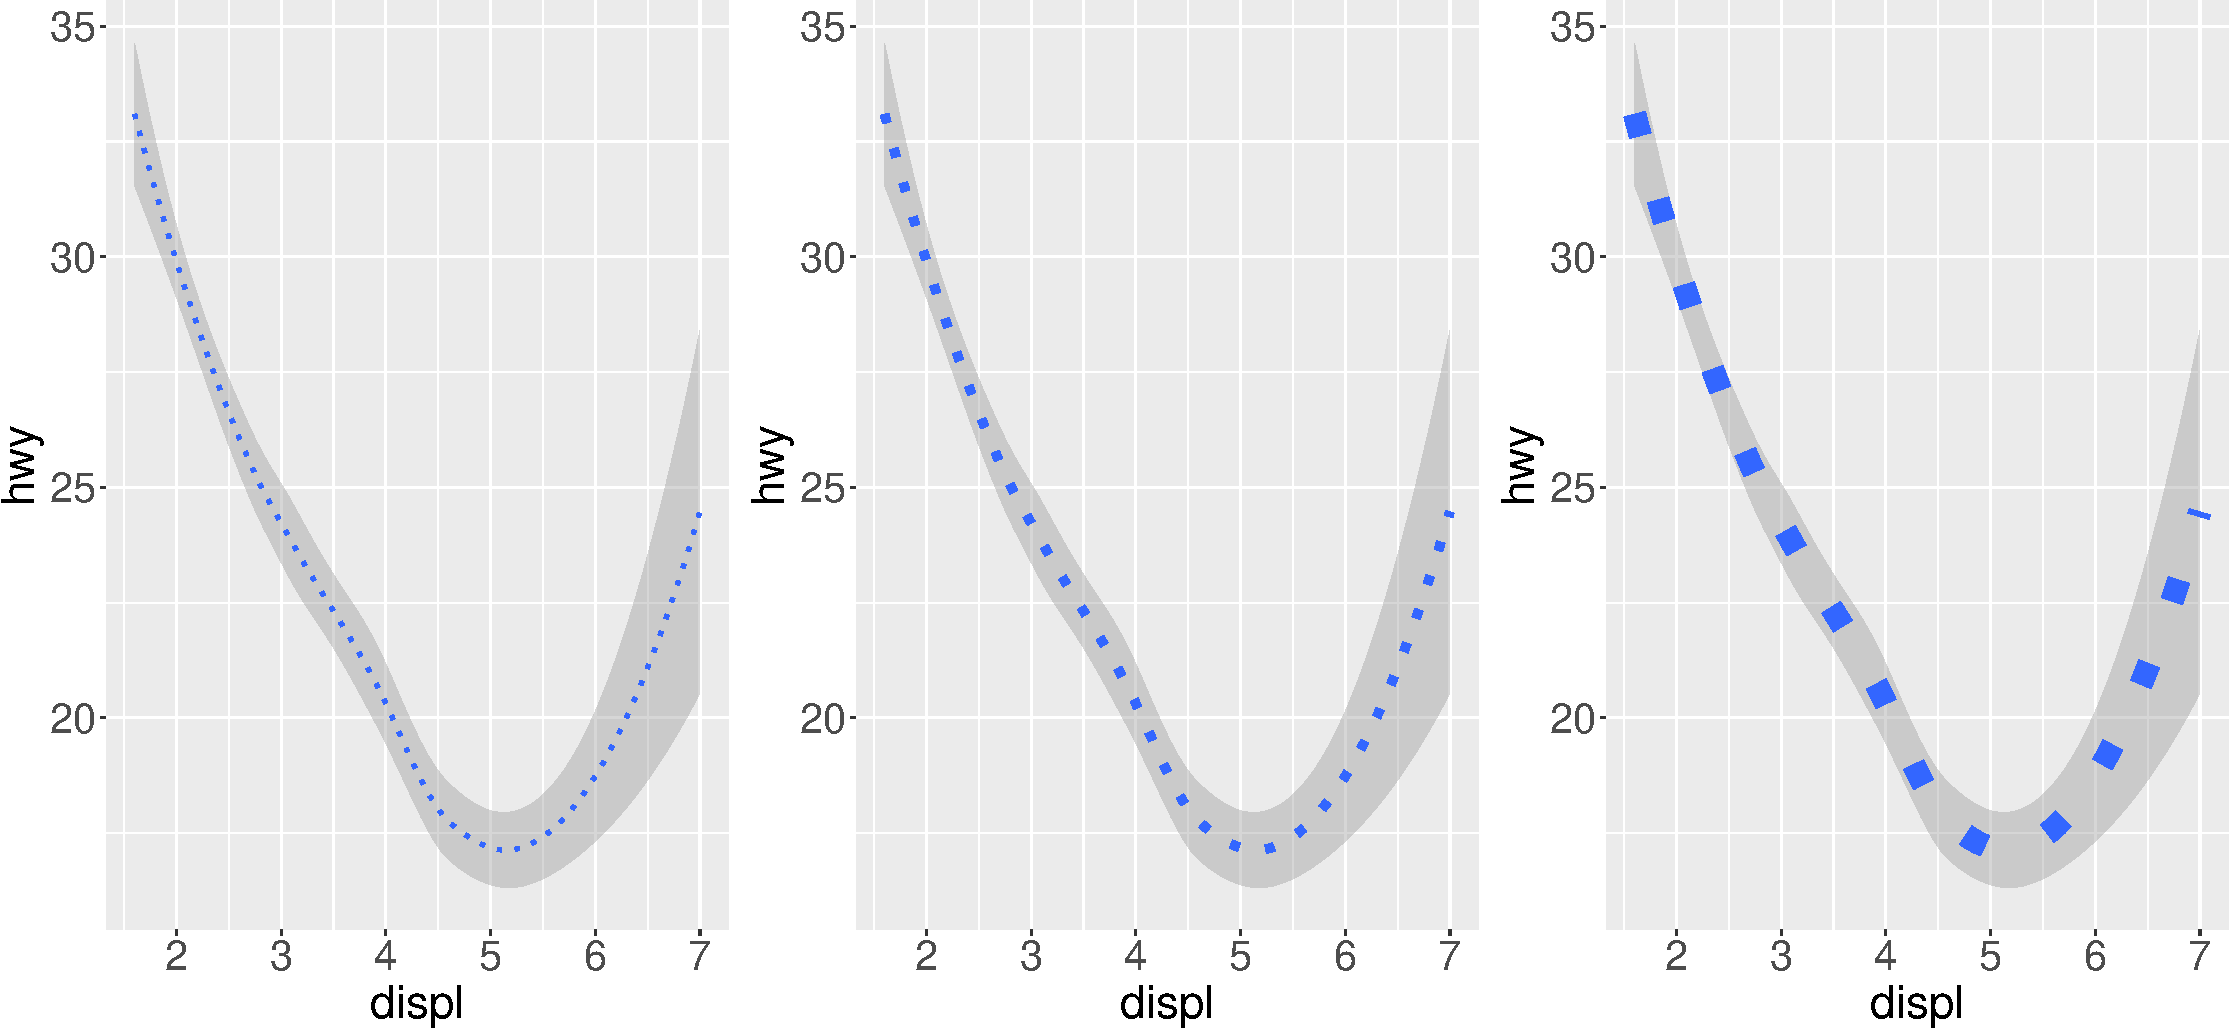
\includegraphics[height=150px]{data-visualization_files/figure-beamer/unnamed-chunk-57-1} \end{center}

\end{frame}

\begin{frame}[fragile]{Changing default aesthetic properties of geoms}
\protect\hypertarget{changing-default-aesthetic-properties-of-geoms-25}{}

\begin{itemize}
\tightlist
\item
  By default, \texttt{geom\_smooth()} displays confidence intervals
  around the smoothed line.
\item
  Confidence intervals may be disabled by setting the \texttt{se}
  (standard error) aesthetic to \texttt{FALSE}:
\end{itemize}

\begin{Shaded}
\begin{Highlighting}[]
\KeywordTok{ggplot}\NormalTok{(}\DataTypeTok{data =}\NormalTok{ mpg) }\OperatorTok{+}
\StringTok{  }\KeywordTok{geom_smooth}\NormalTok{(}\KeywordTok{aes}\NormalTok{(}\DataTypeTok{x =}\NormalTok{ displ, }\DataTypeTok{y =}\NormalTok{ hwy))}

\KeywordTok{ggplot}\NormalTok{(}\DataTypeTok{data =}\NormalTok{ mpg) }\OperatorTok{+}
\StringTok{  }\KeywordTok{geom_smooth}\NormalTok{(}\KeywordTok{aes}\NormalTok{(}\DataTypeTok{x =}\NormalTok{ displ, }\DataTypeTok{y =}\NormalTok{ hwy),}
    \DataTypeTok{se =} \OtherTok{FALSE}\NormalTok{)}
\end{Highlighting}
\end{Shaded}

\end{frame}

\begin{frame}{Changing default aesthetic properties of geoms}
\protect\hypertarget{changing-default-aesthetic-properties-of-geoms-26}{}

\begin{center}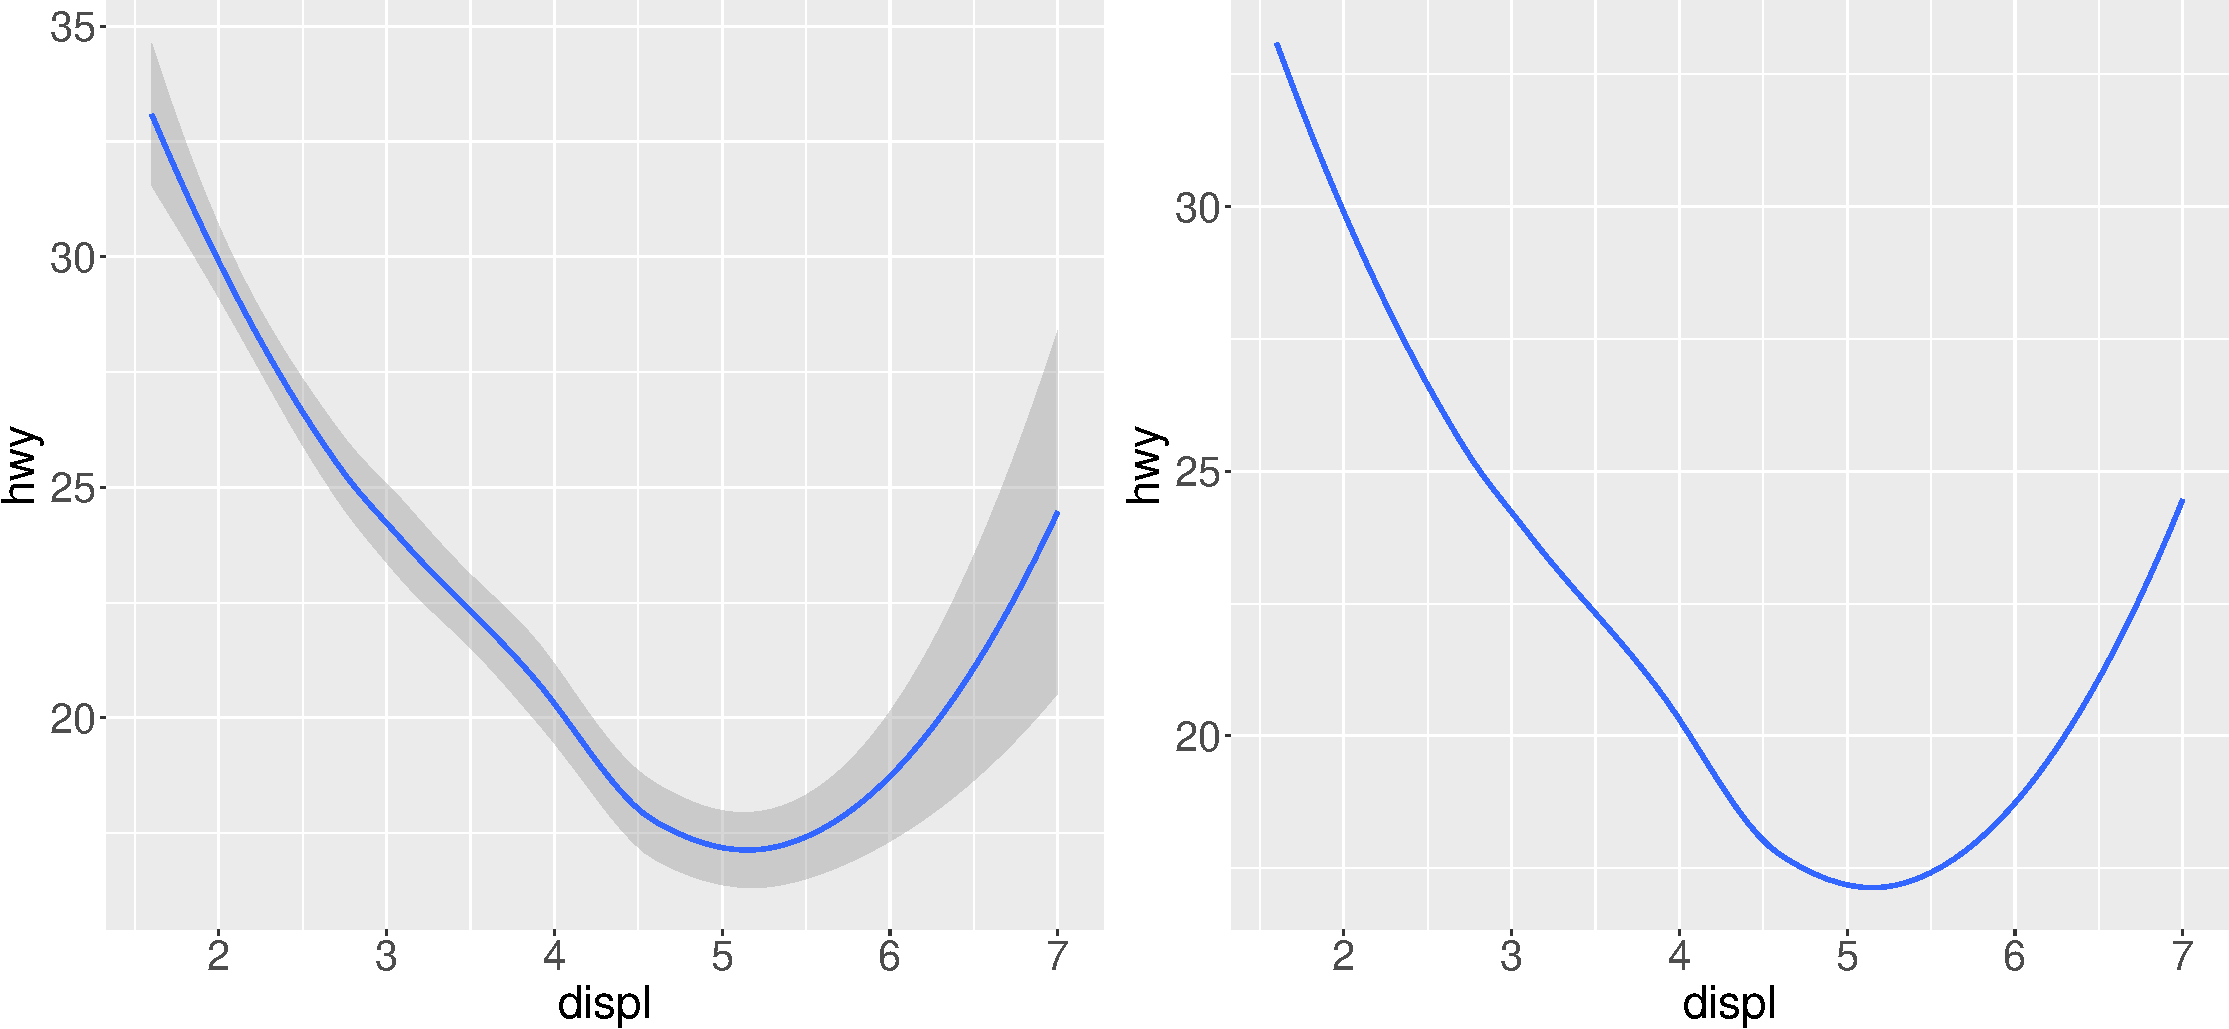
\includegraphics[height=150px]{data-visualization_files/figure-beamer/unnamed-chunk-59-1} \end{center}

\end{frame}

\begin{frame}[fragile]{Changing default aesthetic properties of geoms}
\protect\hypertarget{changing-default-aesthetic-properties-of-geoms-27}{}

\begin{Shaded}
\begin{Highlighting}[]
\KeywordTok{ggplot}\NormalTok{(}\DataTypeTok{data =}\NormalTok{ mpg) }\OperatorTok{+}
\StringTok{  }\KeywordTok{geom_smooth}\NormalTok{(}\KeywordTok{aes}\NormalTok{(}\DataTypeTok{x =}\NormalTok{ displ, }\DataTypeTok{y =}\NormalTok{ hwy, }\DataTypeTok{linetype =}\NormalTok{ drv))}

\KeywordTok{ggplot}\NormalTok{(}\DataTypeTok{data =}\NormalTok{ mpg) }\OperatorTok{+}
\StringTok{  }\KeywordTok{geom_smooth}\NormalTok{(}\KeywordTok{aes}\NormalTok{(}\DataTypeTok{x =}\NormalTok{ displ, }\DataTypeTok{y =}\NormalTok{ hwy, }\DataTypeTok{linetype =}\NormalTok{ drv),}
    \DataTypeTok{se =} \OtherTok{FALSE}\NormalTok{)}
\end{Highlighting}
\end{Shaded}

\end{frame}

\begin{frame}{Changing default aesthetic properties of geoms}
\protect\hypertarget{changing-default-aesthetic-properties-of-geoms-28}{}

\begin{center}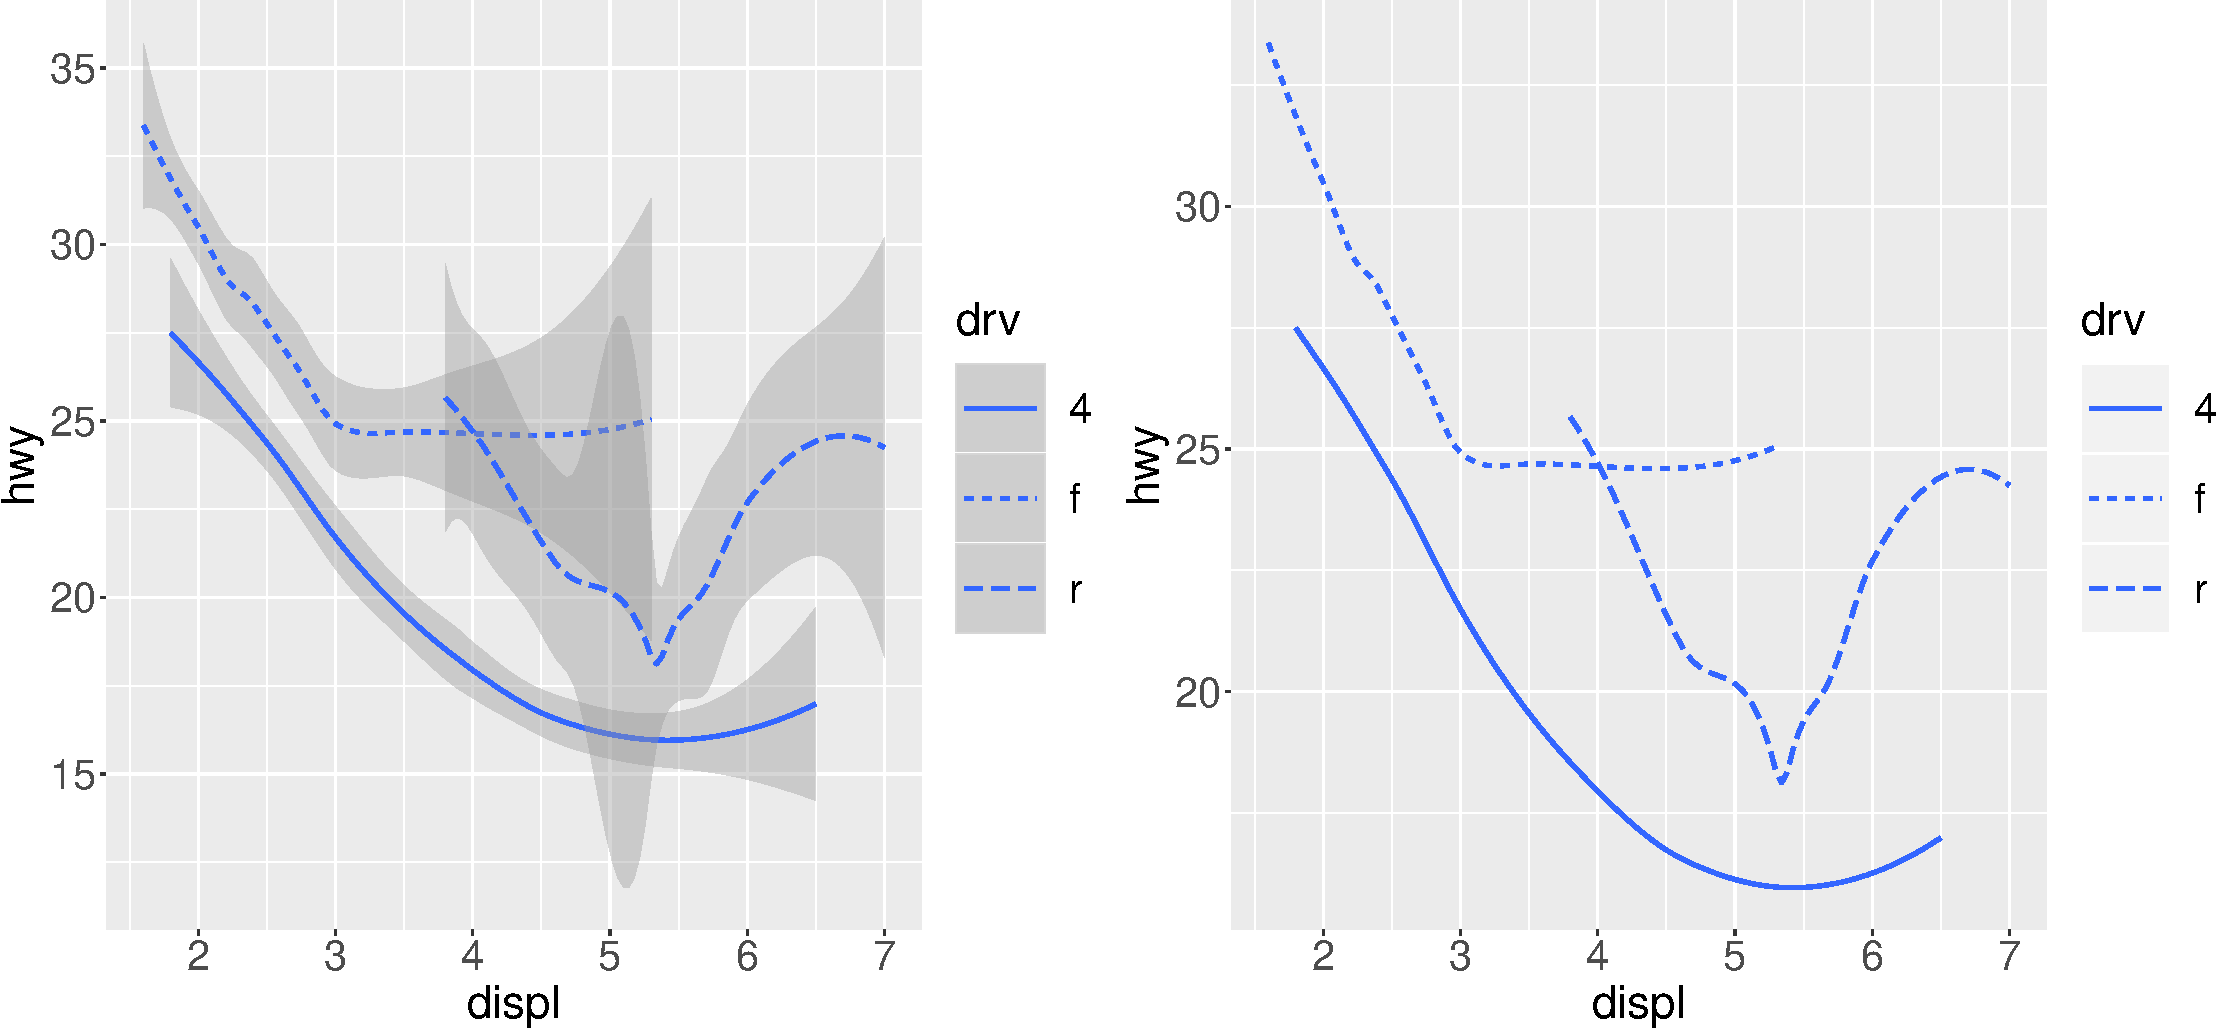
\includegraphics[height=150px]{data-visualization_files/figure-beamer/unnamed-chunk-61-1} \end{center}

\end{frame}

\begin{frame}[fragile]{Changing default aesthetic properties of geoms}
\protect\hypertarget{changing-default-aesthetic-properties-of-geoms-29}{}

\begin{Shaded}
\begin{Highlighting}[]
\KeywordTok{ggplot}\NormalTok{(}\DataTypeTok{data =}\NormalTok{ mpg) }\OperatorTok{+}\StringTok{ }
\StringTok{  }\KeywordTok{geom_smooth}\NormalTok{(}\KeywordTok{aes}\NormalTok{(}\DataTypeTok{x =}\NormalTok{ displ, }\DataTypeTok{y =}\NormalTok{ hwy, }\DataTypeTok{color =}\NormalTok{ drv))}

\KeywordTok{ggplot}\NormalTok{(}\DataTypeTok{data =}\NormalTok{ mpg) }\OperatorTok{+}\StringTok{ }
\StringTok{  }\KeywordTok{geom_smooth}\NormalTok{(}\KeywordTok{aes}\NormalTok{(}\DataTypeTok{x =}\NormalTok{ displ, }\DataTypeTok{y =}\NormalTok{ hwy, }\DataTypeTok{color =}\NormalTok{ drv),}
    \DataTypeTok{se =} \OtherTok{FALSE}\NormalTok{)}
\end{Highlighting}
\end{Shaded}

\end{frame}

\begin{frame}{Changing default aesthetic properties of geoms}
\protect\hypertarget{changing-default-aesthetic-properties-of-geoms-30}{}

\begin{center}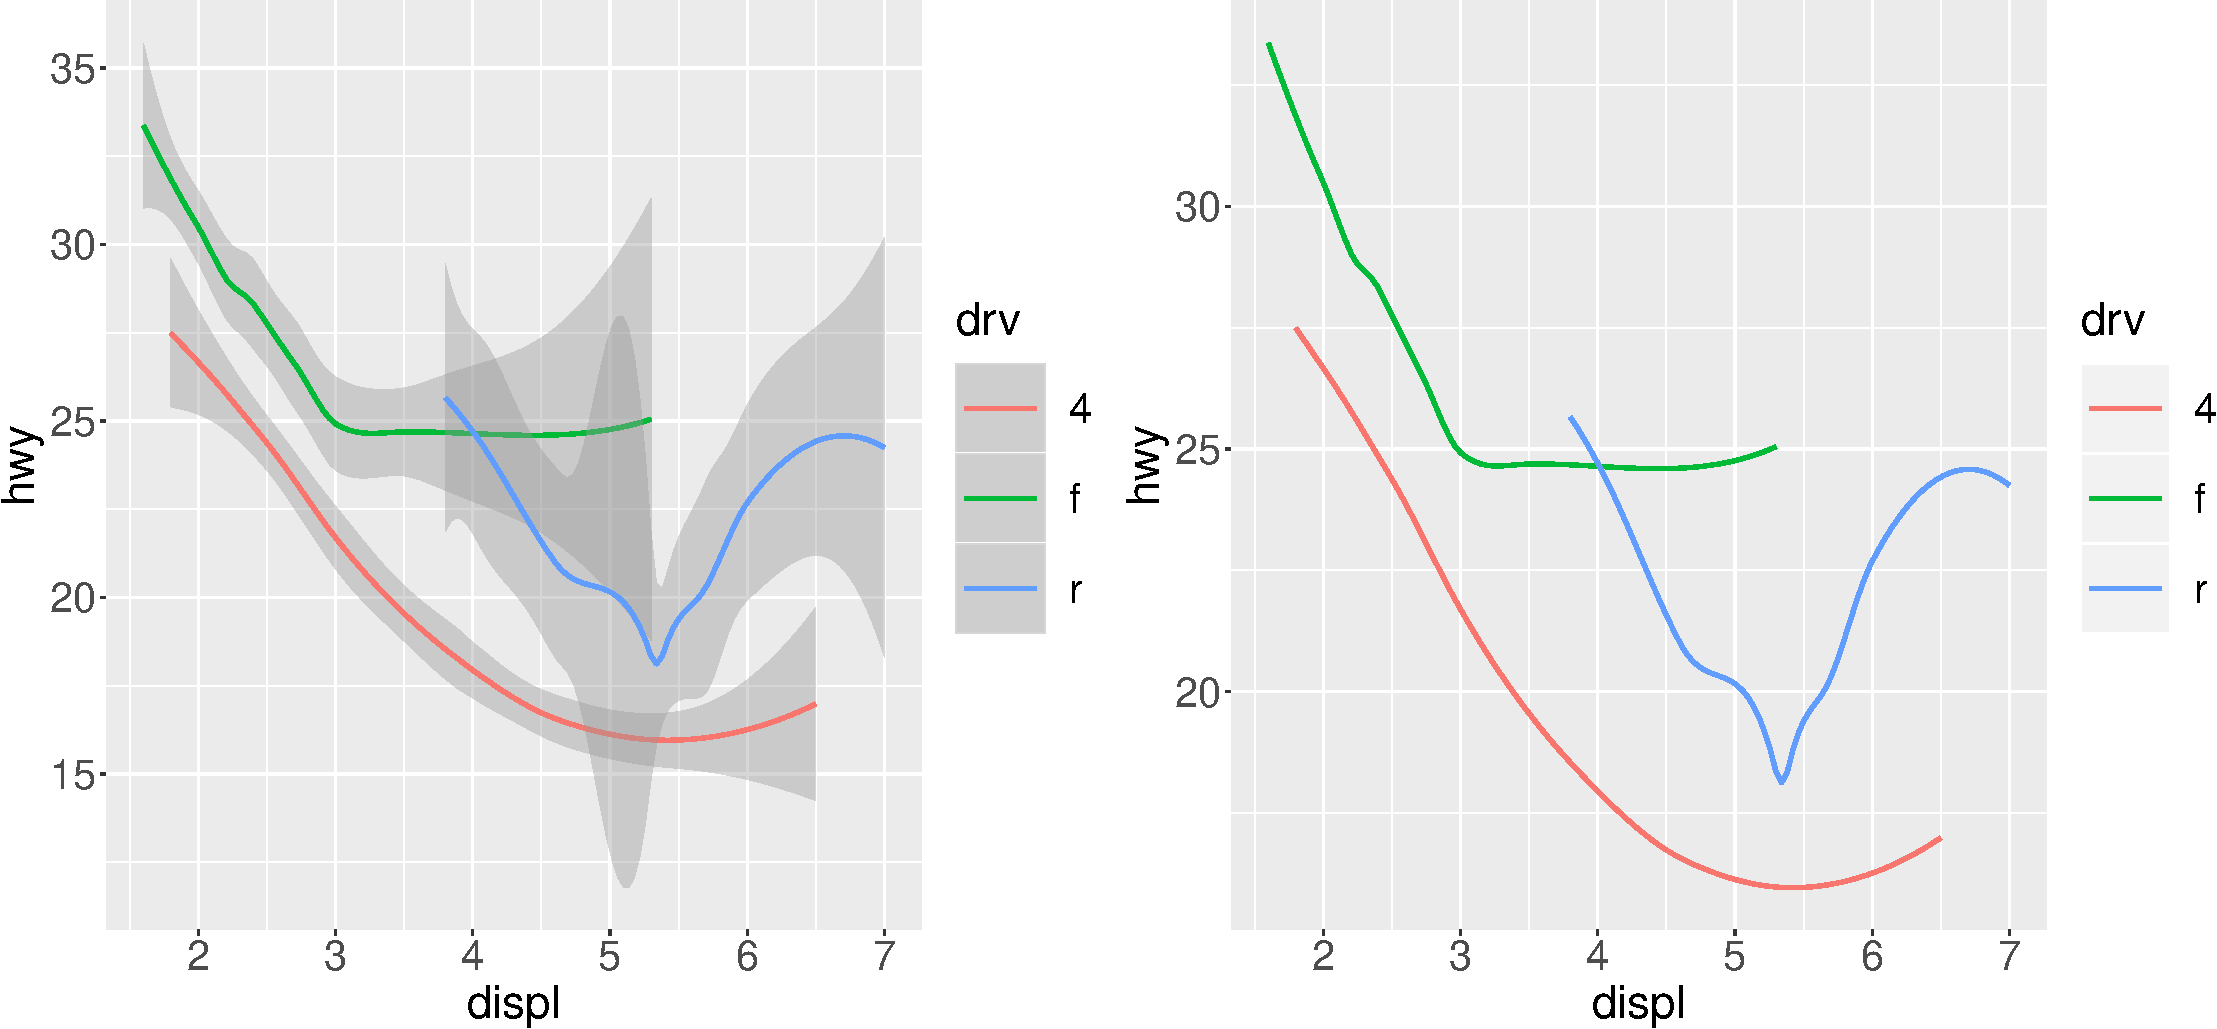
\includegraphics[height=150px]{data-visualization_files/figure-beamer/unnamed-chunk-63-1} \end{center}

\end{frame}

\begin{frame}[fragile]{Changing default aesthetic properties of geoms}
\protect\hypertarget{changing-default-aesthetic-properties-of-geoms-31}{}

\begin{itemize}
\item
  The default smoothing method of \texttt{geom\_smooth} can be changed.
\item
  The default method (\texttt{"auto"}) depends on the size of the
  largest group.
\item
  For less than 1000 obsetvations the method is \texttt{"loess"} (a
  local polynomial regression).
\item
  Admissable methods are: \texttt{"auto"}, \texttt{"lm"},
  \texttt{"glm"}, \texttt{"gam"} and \texttt{"loess"}.
\end{itemize}

\end{frame}

\begin{frame}[fragile]{Changing default aesthetic properties of geoms}
\protect\hypertarget{changing-default-aesthetic-properties-of-geoms-32}{}

To add a linear regression line use \texttt{method\ =\ "lm"}:

\begin{Shaded}
\begin{Highlighting}[]
\KeywordTok{ggplot}\NormalTok{(}\DataTypeTok{data =}\NormalTok{ mpg) }\OperatorTok{+}\StringTok{ }
\StringTok{  }\KeywordTok{geom_point}\NormalTok{(}\KeywordTok{aes}\NormalTok{(}\DataTypeTok{x =}\NormalTok{ displ, }\DataTypeTok{y =}\NormalTok{ hwy))}

\KeywordTok{ggplot}\NormalTok{(}\DataTypeTok{data =}\NormalTok{ mpg) }\OperatorTok{+}\StringTok{ }
\StringTok{  }\KeywordTok{geom_smooth}\NormalTok{(}\KeywordTok{aes}\NormalTok{(}\DataTypeTok{x =}\NormalTok{ displ, }\DataTypeTok{y =}\NormalTok{ hwy))}

\KeywordTok{ggplot}\NormalTok{(}\DataTypeTok{data =}\NormalTok{ mpg) }\OperatorTok{+}\StringTok{ }
\StringTok{  }\KeywordTok{geom_smooth}\NormalTok{(}\KeywordTok{aes}\NormalTok{(}\DataTypeTok{x =}\NormalTok{ displ, }\DataTypeTok{y =}\NormalTok{ hwy), }\DataTypeTok{method =} \StringTok{"lm"}\NormalTok{)}
\end{Highlighting}
\end{Shaded}

\end{frame}

\begin{frame}{Changing default aesthetic properties of geoms}
\protect\hypertarget{changing-default-aesthetic-properties-of-geoms-33}{}

\begin{center}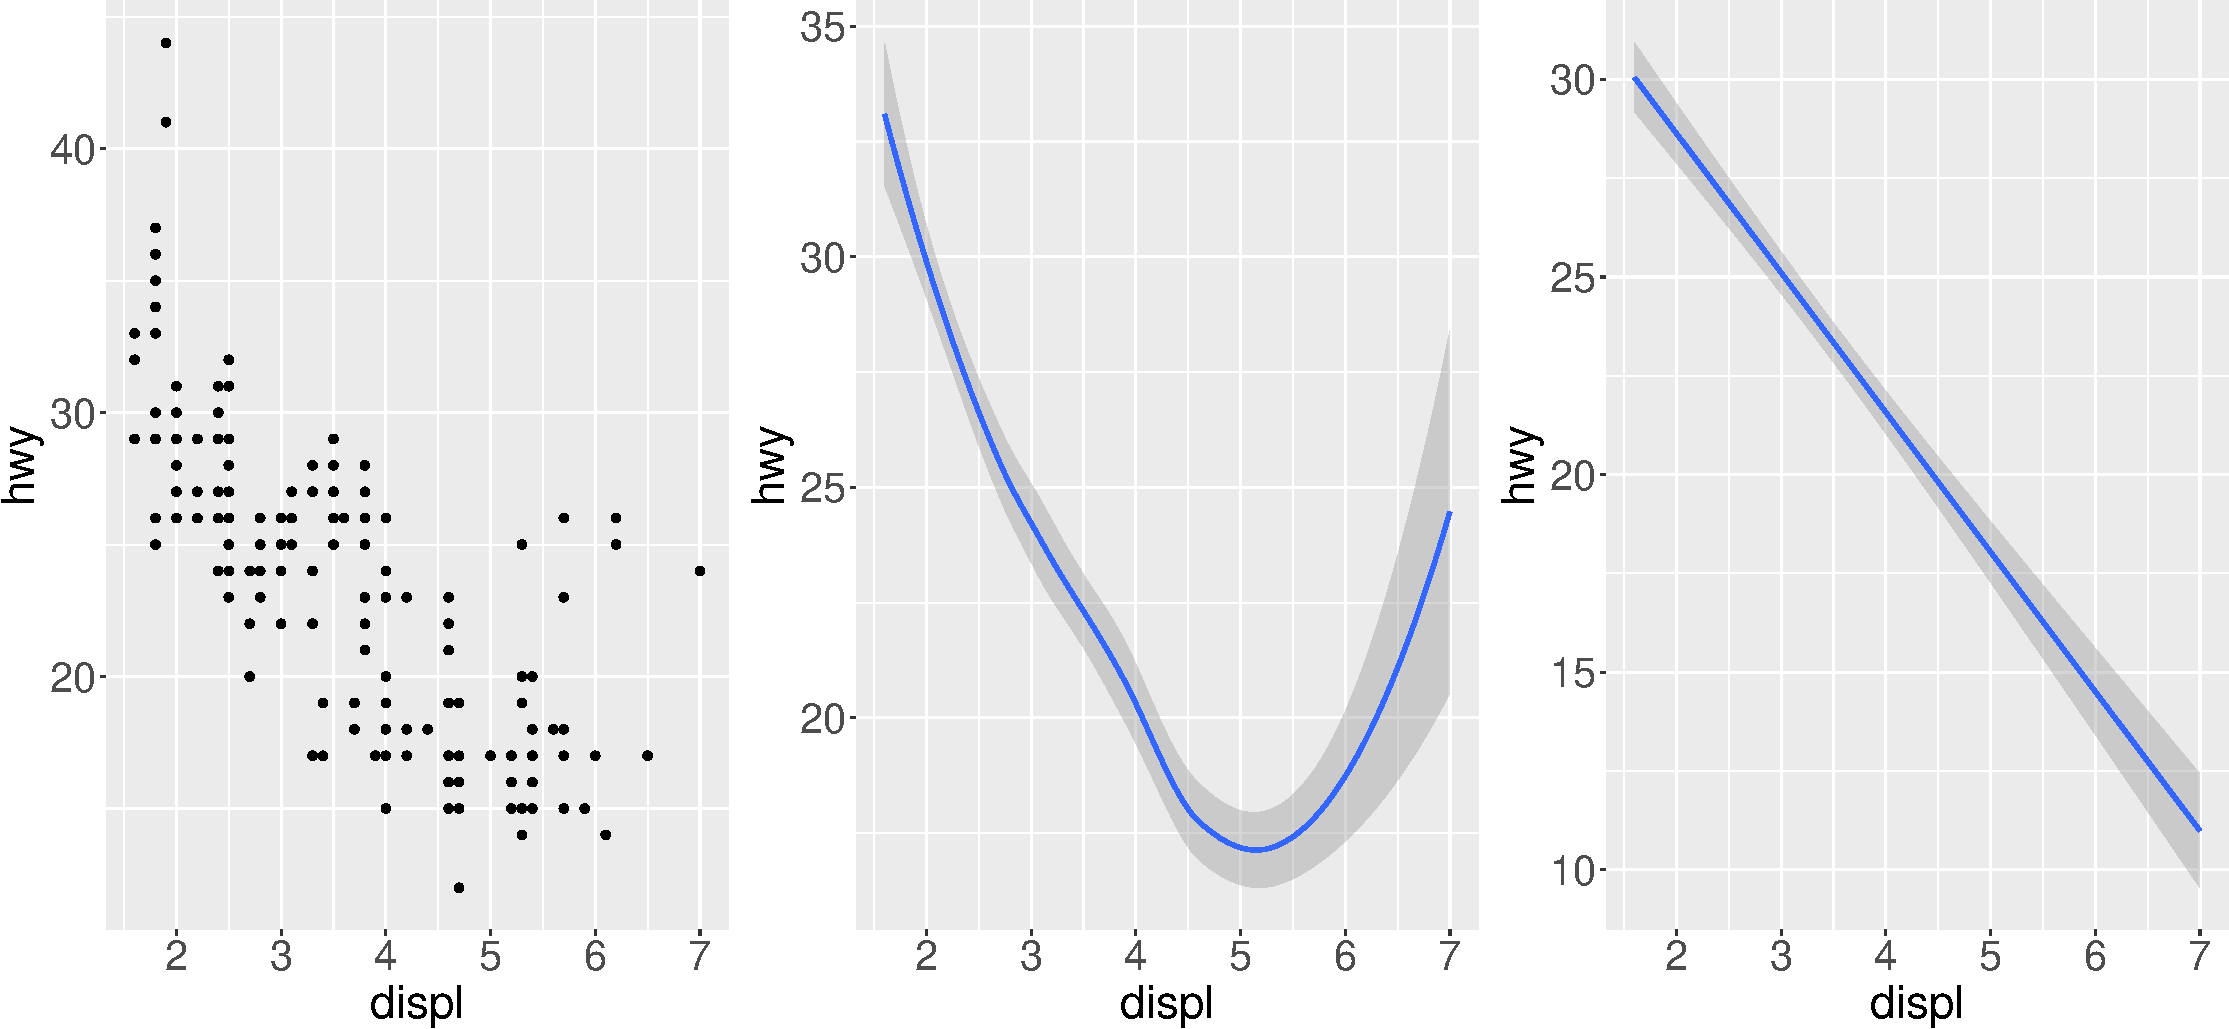
\includegraphics[height=150px]{data-visualization_files/figure-beamer/unnamed-chunk-65-1} \end{center}

\end{frame}

\begin{frame}[fragile]{Changing default aesthetic properties of geoms}
\protect\hypertarget{changing-default-aesthetic-properties-of-geoms-34}{}

Legends can also be disabled:

\begin{Shaded}
\begin{Highlighting}[]
\KeywordTok{ggplot}\NormalTok{(}\DataTypeTok{data =}\NormalTok{ mpg) }\OperatorTok{+}\StringTok{ }
\StringTok{  }\KeywordTok{geom_smooth}\NormalTok{(}\KeywordTok{aes}\NormalTok{(}\DataTypeTok{x =}\NormalTok{ displ, }\DataTypeTok{y =}\NormalTok{ hwy, }\DataTypeTok{linetype =}\NormalTok{ drv),}
    \DataTypeTok{se =} \OtherTok{FALSE}\NormalTok{)}

\KeywordTok{ggplot}\NormalTok{(}\DataTypeTok{data =}\NormalTok{ mpg) }\OperatorTok{+}\StringTok{ }
\StringTok{  }\KeywordTok{geom_smooth}\NormalTok{(}\KeywordTok{aes}\NormalTok{(}\DataTypeTok{x =}\NormalTok{ displ, }\DataTypeTok{y =}\NormalTok{ hwy, }\DataTypeTok{linetype =}\NormalTok{ drv),}
    \DataTypeTok{se =} \OtherTok{FALSE}\NormalTok{, }\DataTypeTok{show.legend =} \OtherTok{FALSE}\NormalTok{)}
\end{Highlighting}
\end{Shaded}

\end{frame}

\begin{frame}{Changing default aesthetic properties of geoms}
\protect\hypertarget{changing-default-aesthetic-properties-of-geoms-35}{}

\begin{center}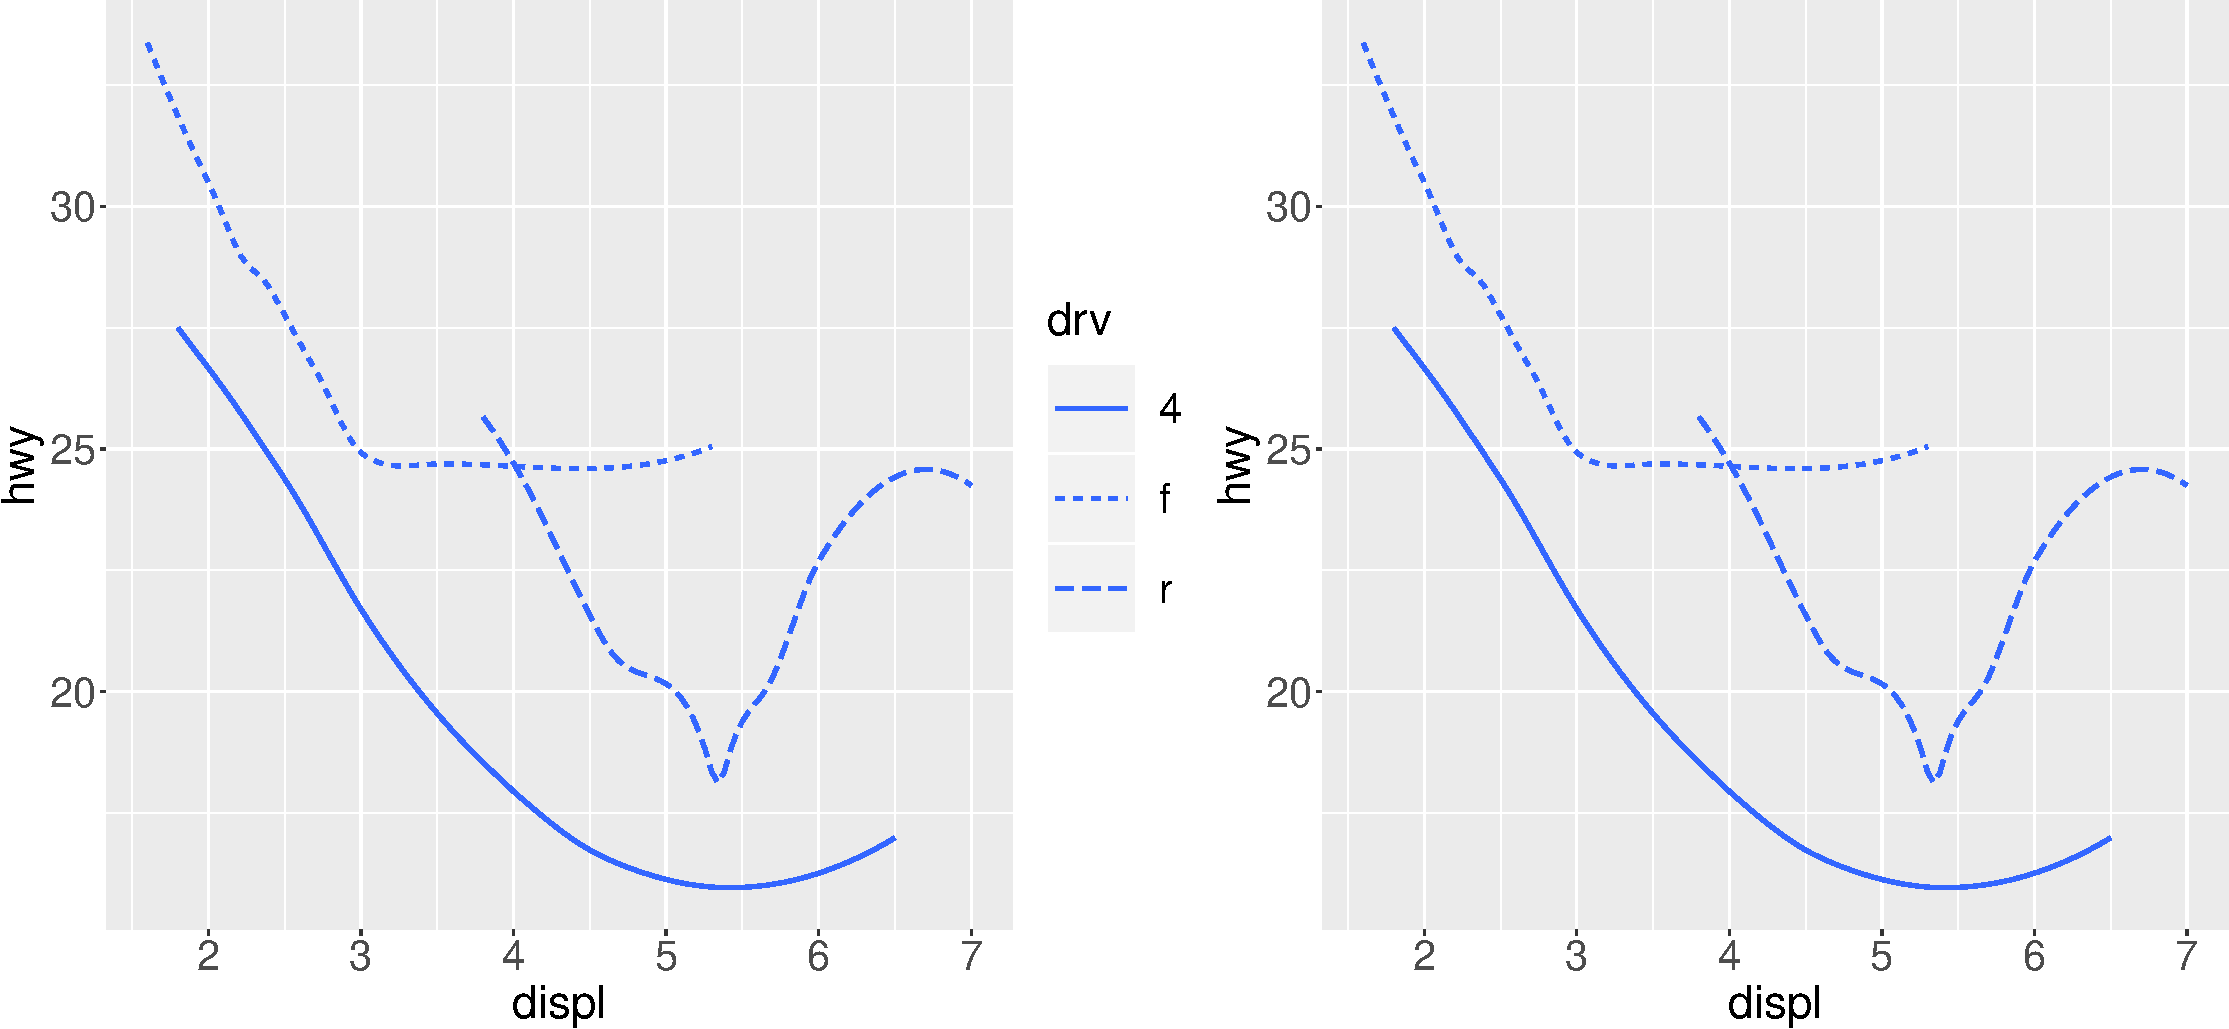
\includegraphics[height=150px]{data-visualization_files/figure-beamer/unnamed-chunk-67-1} \end{center}

\end{frame}

\begin{frame}[fragile]{Changing default aesthetic properties of geoms}
\protect\hypertarget{changing-default-aesthetic-properties-of-geoms-36}{}

\begin{Shaded}
\begin{Highlighting}[]
\KeywordTok{ggplot}\NormalTok{(}\DataTypeTok{data =}\NormalTok{ mpg) }\OperatorTok{+}\StringTok{ }
\StringTok{  }\KeywordTok{geom_smooth}\NormalTok{(}\KeywordTok{aes}\NormalTok{(}\DataTypeTok{x =}\NormalTok{ displ, }\DataTypeTok{y =}\NormalTok{ hwy, }\DataTypeTok{color =}\NormalTok{ drv),}
    \DataTypeTok{se =} \OtherTok{FALSE}\NormalTok{)}

\KeywordTok{ggplot}\NormalTok{(}\DataTypeTok{data =}\NormalTok{ mpg) }\OperatorTok{+}\StringTok{ }
\StringTok{  }\KeywordTok{geom_smooth}\NormalTok{(}\KeywordTok{aes}\NormalTok{(}\DataTypeTok{x =}\NormalTok{ displ, }\DataTypeTok{y =}\NormalTok{ hwy, }\DataTypeTok{color =}\NormalTok{ drv),}
    \DataTypeTok{se =} \OtherTok{FALSE}\NormalTok{, }\DataTypeTok{show.legend =} \OtherTok{FALSE}\NormalTok{)}
\end{Highlighting}
\end{Shaded}

\end{frame}

\begin{frame}{Changing default aesthetic properties of geoms}
\protect\hypertarget{changing-default-aesthetic-properties-of-geoms-37}{}

\begin{center}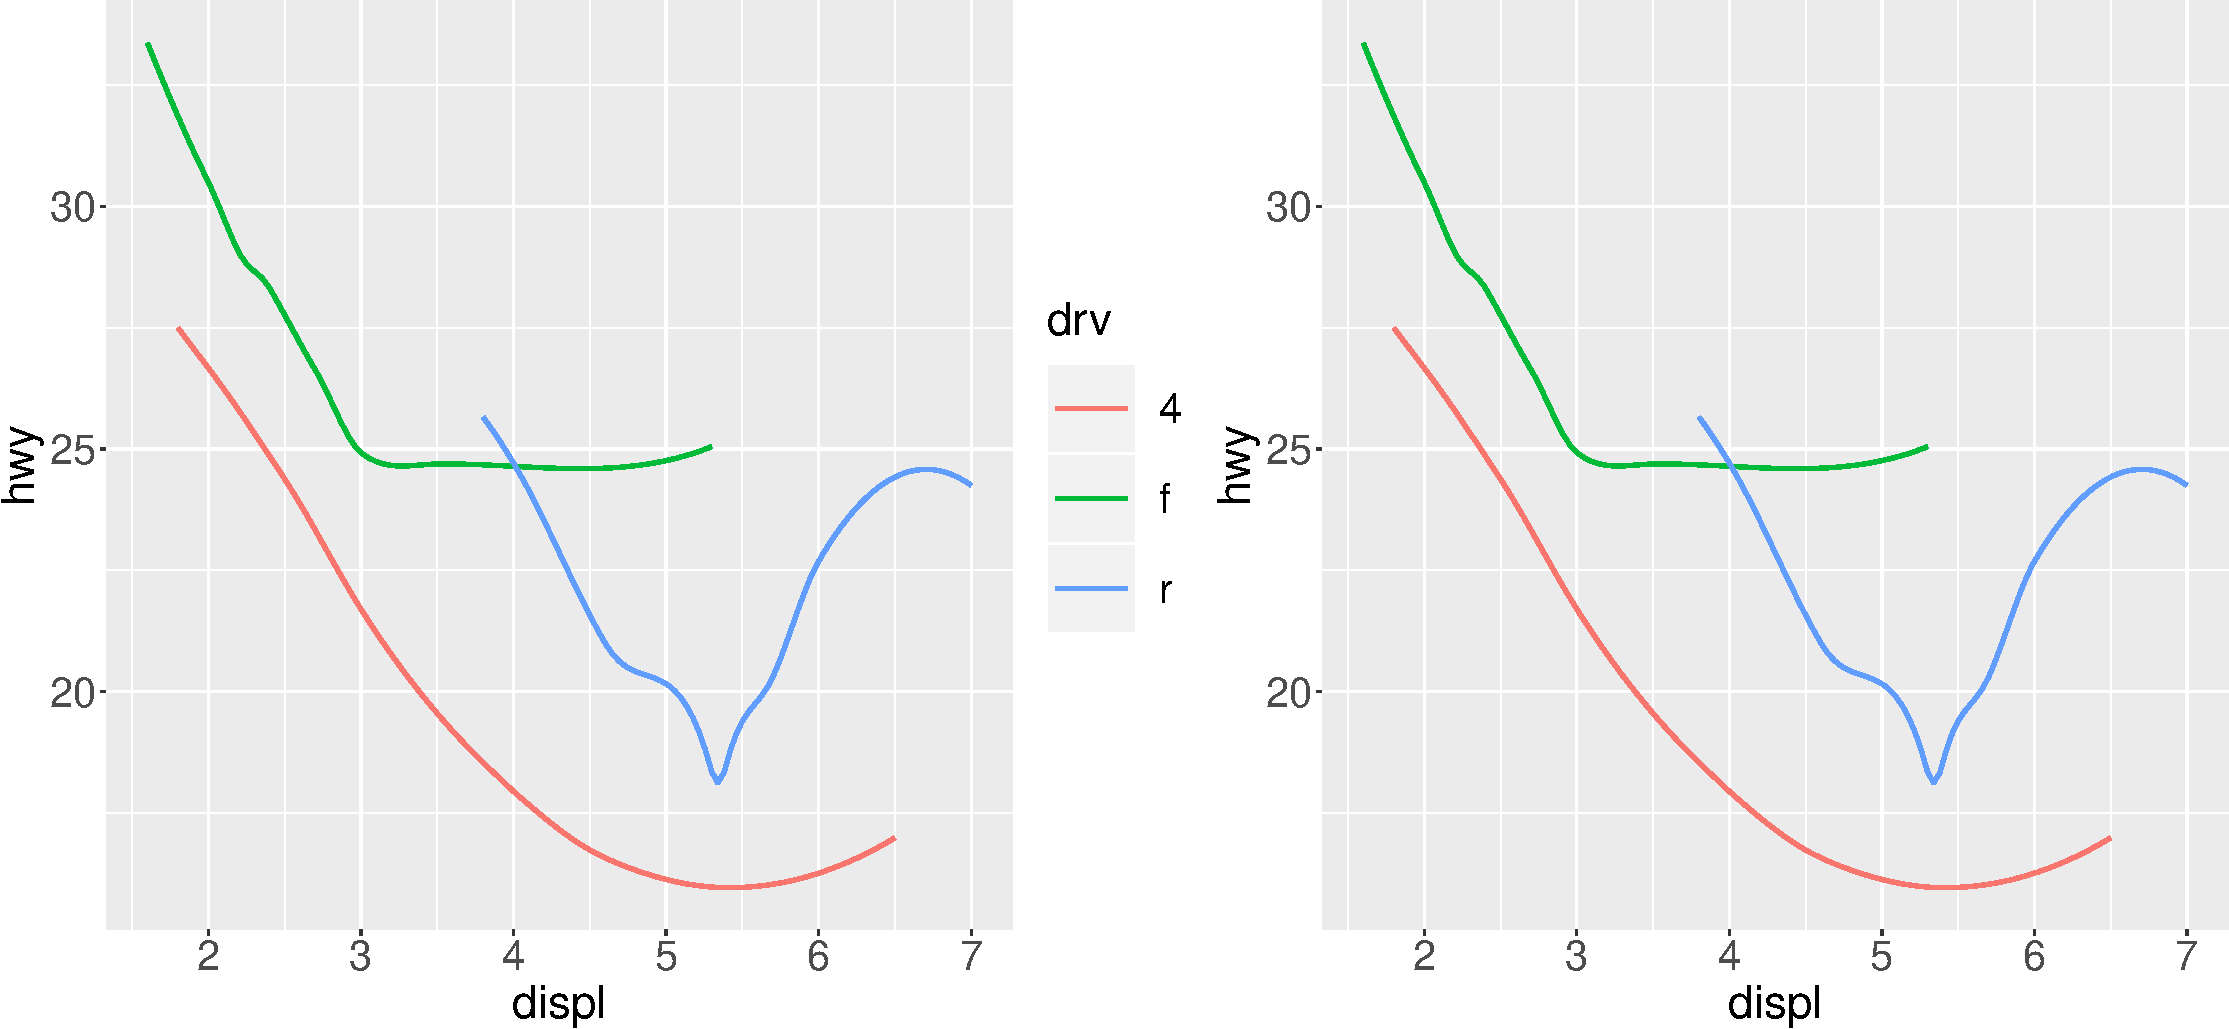
\includegraphics[height=150px]{data-visualization_files/figure-beamer/unnamed-chunk-69-1} \end{center}

\end{frame}

\begin{frame}[fragile]{Facets}
\protect\hypertarget{facets}{}

\begin{itemize}
\item
  One way to add additional variables to a plot is with
  \textbf{aesthetics}.
\item
  Another way, particularly useful for categorical variables, is to
  split your plot into \textbf{facets}, subplots that each display one
  subset of the data.
\item
  To facet your plot by a single variable, use \texttt{facet\_wrap()}.
\item
  The first argument of \texttt{facet\_wrap()} should be
  \texttt{"\textasciitilde{}}" followed the name of a variable.
\end{itemize}

\end{frame}

\begin{frame}[fragile]{Facets}
\protect\hypertarget{facets-1}{}

\begin{Shaded}
\begin{Highlighting}[]
\KeywordTok{ggplot}\NormalTok{(}\DataTypeTok{data =}\NormalTok{ mpg) }\OperatorTok{+}\StringTok{ }
\StringTok{  }\KeywordTok{geom_point}\NormalTok{(}\KeywordTok{aes}\NormalTok{(}\DataTypeTok{x =}\NormalTok{ displ, }\DataTypeTok{y =}\NormalTok{ hwy)) }\OperatorTok{+}\StringTok{ }
\StringTok{  }\KeywordTok{facet_wrap}\NormalTok{(}\OperatorTok{~}\StringTok{ }\NormalTok{class, }\DataTypeTok{nrow =} \DecValTok{2}\NormalTok{)}
\end{Highlighting}
\end{Shaded}

\end{frame}

\begin{frame}{Facets}
\protect\hypertarget{facets-2}{}

\begin{center}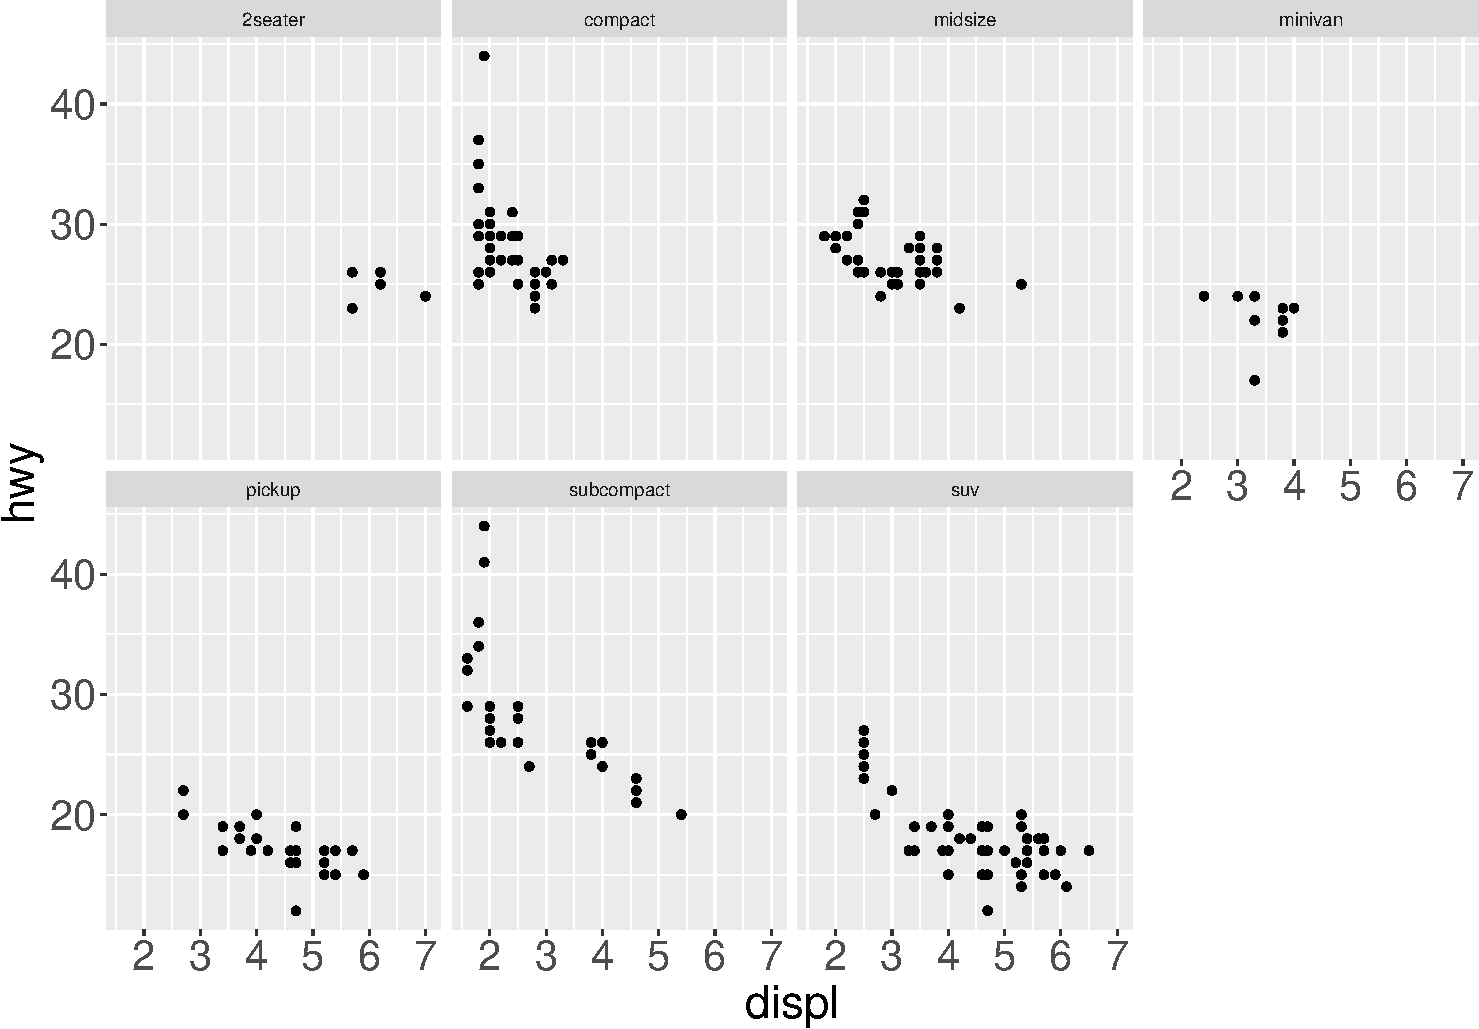
\includegraphics[height=200px]{data-visualization_files/figure-beamer/unnamed-chunk-71-1} \end{center}

\end{frame}

\begin{frame}[fragile]{Facets}
\protect\hypertarget{facets-3}{}

\begin{Shaded}
\begin{Highlighting}[]
\KeywordTok{ggplot}\NormalTok{(}\DataTypeTok{data =}\NormalTok{ mpg) }\OperatorTok{+}\StringTok{ }
\StringTok{  }\KeywordTok{geom_smooth}\NormalTok{(}\KeywordTok{aes}\NormalTok{(}\DataTypeTok{x =}\NormalTok{ displ, }\DataTypeTok{y =}\NormalTok{ cyl), }\DataTypeTok{se =} \OtherTok{FALSE}\NormalTok{) }\OperatorTok{+}\StringTok{ }
\StringTok{  }\KeywordTok{facet_wrap}\NormalTok{(}\OperatorTok{~}\NormalTok{class, }\DataTypeTok{nrow =} \DecValTok{2}\NormalTok{)}
\end{Highlighting}
\end{Shaded}

\end{frame}

\begin{frame}{Facets}
\protect\hypertarget{facets-4}{}

\begin{center}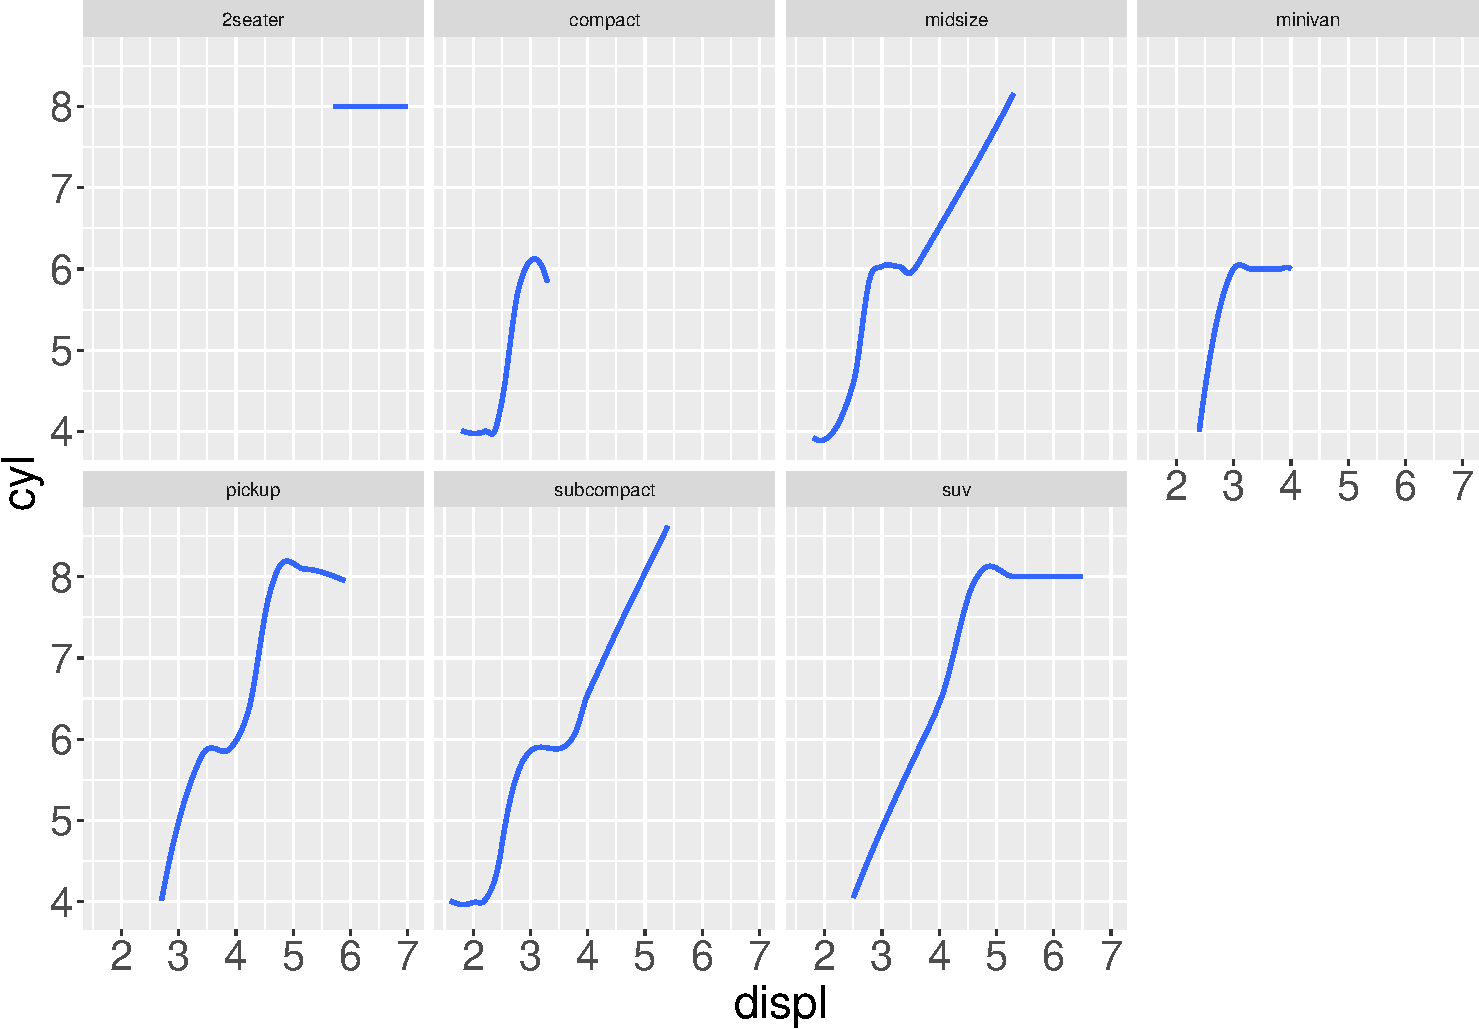
\includegraphics[height=200px]{data-visualization_files/figure-beamer/unnamed-chunk-73-1} \end{center}

\end{frame}

\begin{frame}[fragile]{Facets}
\protect\hypertarget{facets-5}{}

\begin{itemize}
\item
  To facet your plot on the combination of two variables, use
  \texttt{facet\_grid()}.
\item
  The first argument of \texttt{facet\_grid()} should contain the two
  variable names separated by \texttt{"\textasciitilde{}"}.
\end{itemize}

\begin{Shaded}
\begin{Highlighting}[]
\KeywordTok{ggplot}\NormalTok{(}\DataTypeTok{data =}\NormalTok{ mpg) }\OperatorTok{+}\StringTok{ }
\StringTok{  }\KeywordTok{geom_point}\NormalTok{(}\KeywordTok{aes}\NormalTok{(}\DataTypeTok{x =}\NormalTok{ displ, }\DataTypeTok{y =}\NormalTok{ hwy)) }\OperatorTok{+}\StringTok{ }
\StringTok{  }\KeywordTok{facet_grid}\NormalTok{(drv }\OperatorTok{~}\StringTok{ }\NormalTok{cyl)}
\end{Highlighting}
\end{Shaded}

\end{frame}

\begin{frame}{Facets}
\protect\hypertarget{facets-6}{}

\begin{center}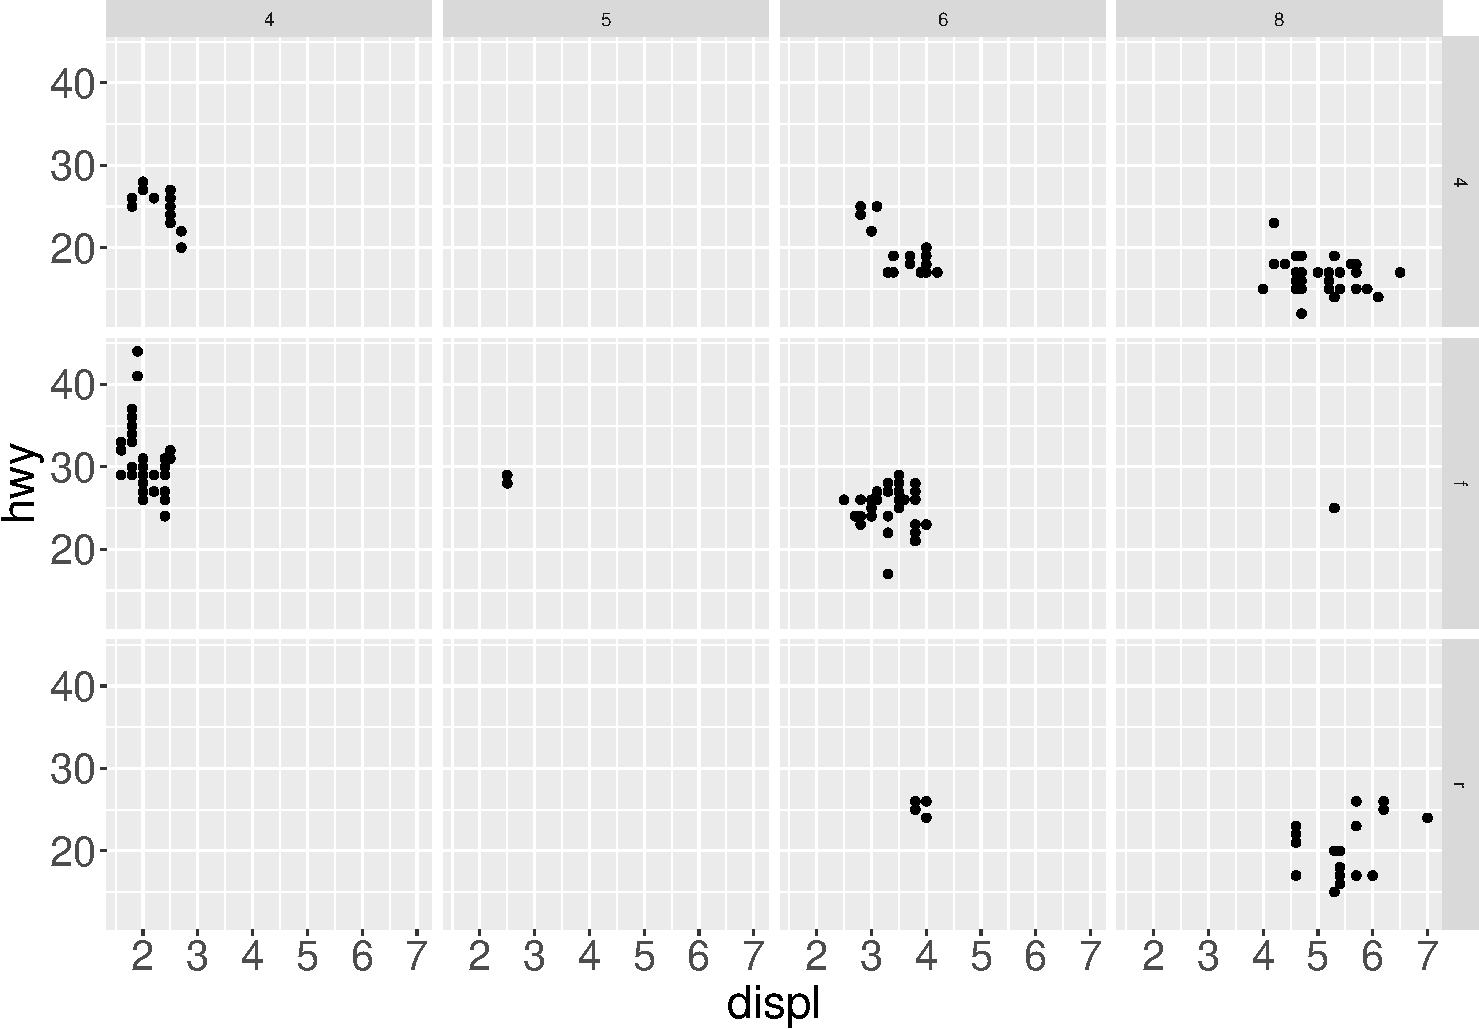
\includegraphics[height=200px]{data-visualization_files/figure-beamer/unnamed-chunk-75-1} \end{center}

\end{frame}

\begin{frame}[fragile]{Facets}
\protect\hypertarget{facets-7}{}

If you prefer to not facet in the rows (or columns), use a \texttt{"."}
instead of a variable name:

\begin{Shaded}
\begin{Highlighting}[]
\KeywordTok{ggplot}\NormalTok{(}\DataTypeTok{data =}\NormalTok{ mpg) }\OperatorTok{+}\StringTok{ }
\StringTok{  }\KeywordTok{geom_point}\NormalTok{(}\KeywordTok{aes}\NormalTok{(}\DataTypeTok{x =}\NormalTok{ displ, }\DataTypeTok{y =}\NormalTok{ hwy)) }\OperatorTok{+}\StringTok{ }
\StringTok{  }\KeywordTok{facet_grid}\NormalTok{(. }\OperatorTok{~}\StringTok{ }\NormalTok{cyl)}
\end{Highlighting}
\end{Shaded}

\end{frame}

\begin{frame}{Facets}
\protect\hypertarget{facets-8}{}

\begin{center}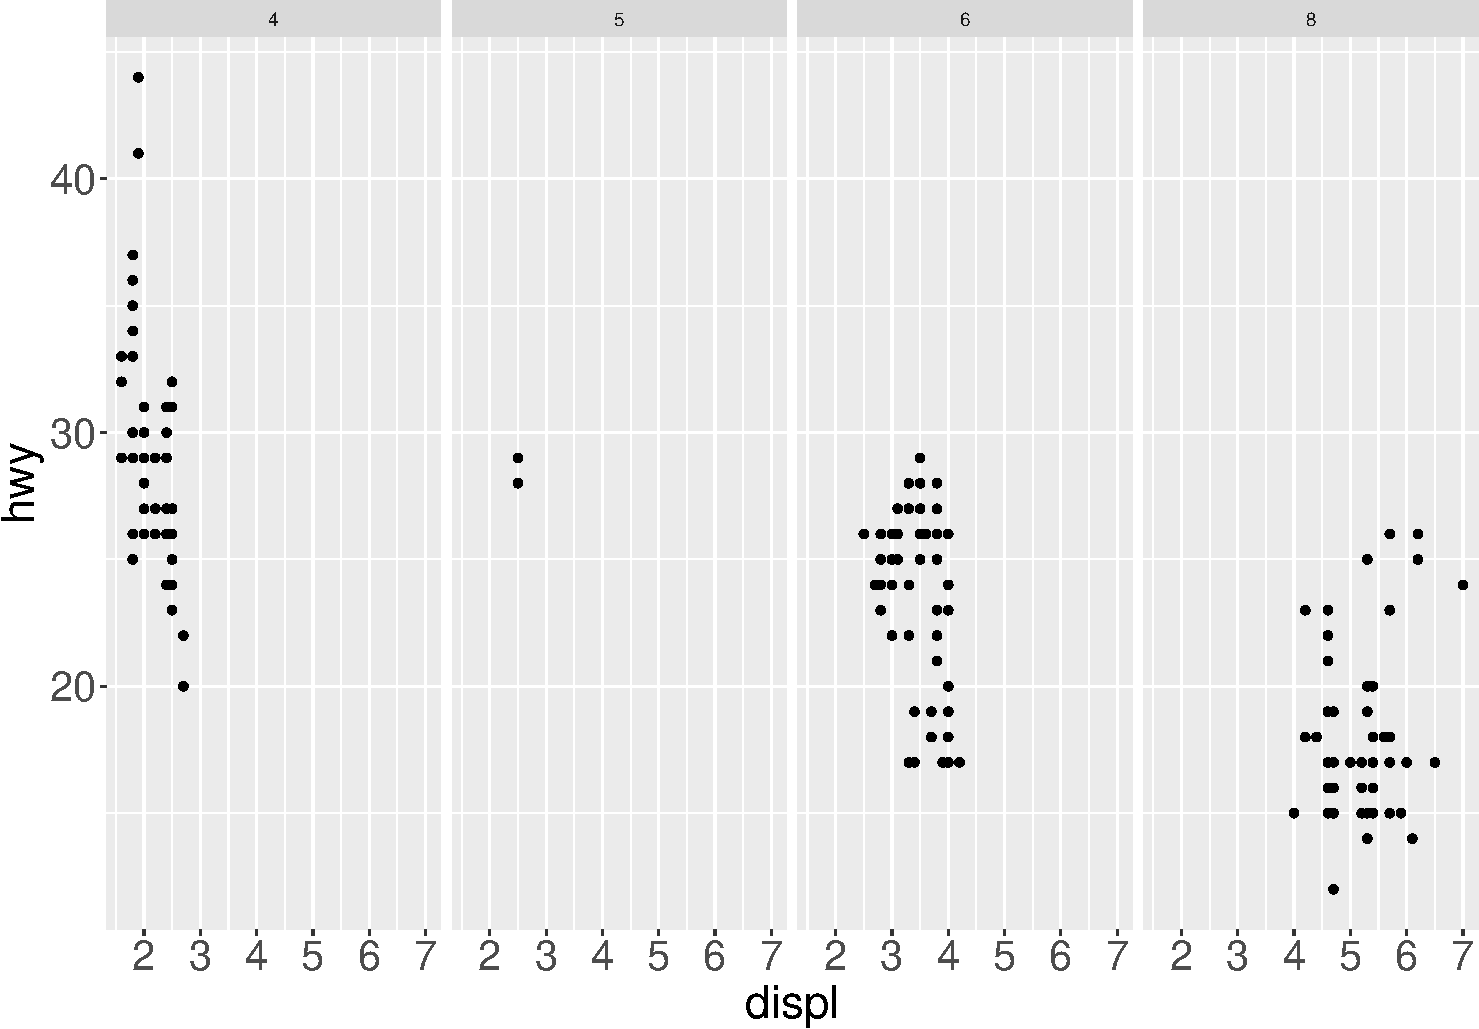
\includegraphics[height=200px]{data-visualization_files/figure-beamer/unnamed-chunk-77-1} \end{center}

\end{frame}

\begin{frame}[fragile]{Facets}
\protect\hypertarget{facets-9}{}

\begin{Shaded}
\begin{Highlighting}[]
\KeywordTok{ggplot}\NormalTok{(}\DataTypeTok{data =}\NormalTok{ mpg) }\OperatorTok{+}\StringTok{ }
\StringTok{  }\KeywordTok{geom_point}\NormalTok{(}\KeywordTok{aes}\NormalTok{(}\DataTypeTok{x =}\NormalTok{ displ, }\DataTypeTok{y =}\NormalTok{ hwy)) }\OperatorTok{+}
\StringTok{  }\KeywordTok{facet_grid}\NormalTok{(drv }\OperatorTok{~}\StringTok{ }\NormalTok{.)}
\end{Highlighting}
\end{Shaded}

\end{frame}

\begin{frame}{Facets}
\protect\hypertarget{facets-10}{}

\begin{center}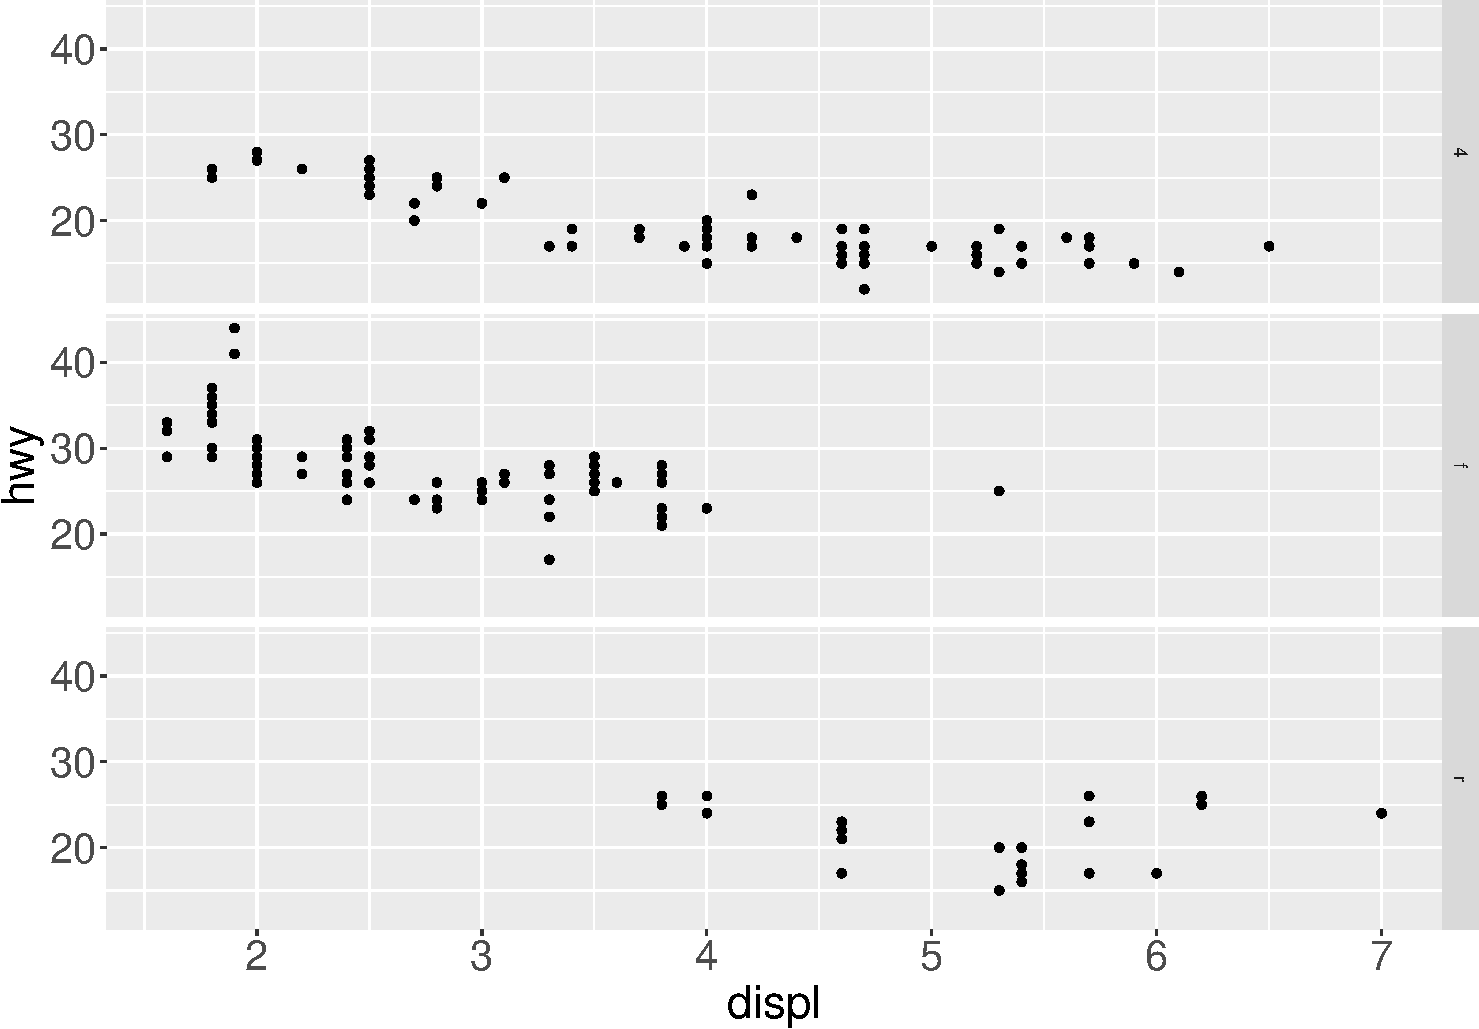
\includegraphics[height=200px]{data-visualization_files/figure-beamer/unnamed-chunk-79-1} \end{center}

\end{frame}

\begin{frame}[fragile]{Multiple geoms}
\protect\hypertarget{multiple-geoms}{}

\begin{itemize}
\item
  We can add multiple geoms to the same graph.
\item
  For example, we can overlap points and lines.
\item
  This is archieved by adding multiple geom functions to
  \texttt{ggplot()}.
\end{itemize}

\end{frame}

\begin{frame}[fragile]{Multiple geoms}
\protect\hypertarget{multiple-geoms-1}{}

\begin{Shaded}
\begin{Highlighting}[]
\KeywordTok{ggplot}\NormalTok{(}\DataTypeTok{data =}\NormalTok{ mpg) }\OperatorTok{+}\StringTok{ }
\StringTok{  }\KeywordTok{geom_point}\NormalTok{(}\KeywordTok{aes}\NormalTok{(}\DataTypeTok{x =}\NormalTok{ displ, }\DataTypeTok{y =}\NormalTok{ hwy)) }\OperatorTok{+}
\StringTok{  }\KeywordTok{geom_smooth}\NormalTok{(}\KeywordTok{aes}\NormalTok{(}\DataTypeTok{x =}\NormalTok{ displ, }\DataTypeTok{y =}\NormalTok{ hwy))}
\end{Highlighting}
\end{Shaded}

\begin{center}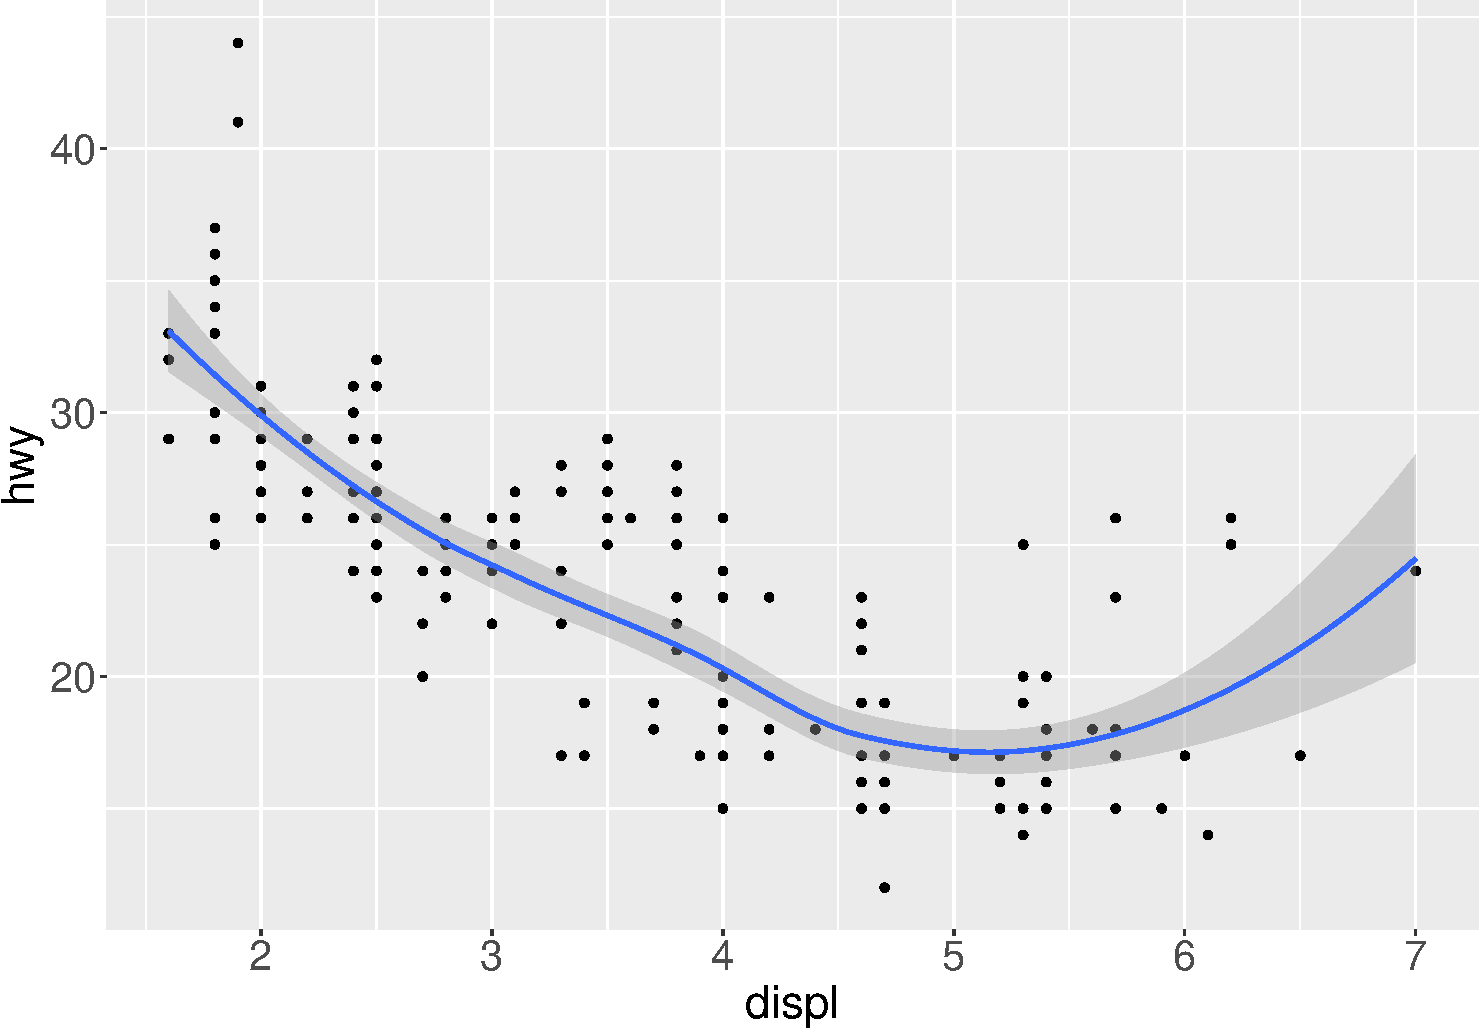
\includegraphics[height=150px]{data-visualization_files/figure-beamer/unnamed-chunk-80-1} \end{center}

\end{frame}

\begin{frame}[fragile]{Multiple geoms}
\protect\hypertarget{multiple-geoms-2}{}

\begin{Shaded}
\begin{Highlighting}[]
\KeywordTok{ggplot}\NormalTok{(}\DataTypeTok{data =}\NormalTok{ mpg) }\OperatorTok{+}
\StringTok{  }\KeywordTok{geom_smooth}\NormalTok{(}\KeywordTok{aes}\NormalTok{(}\DataTypeTok{x =}\NormalTok{ displ, }\DataTypeTok{y =}\NormalTok{ hwy), }\DataTypeTok{se =} \OtherTok{FALSE}\NormalTok{) }\OperatorTok{+}
\StringTok{  }\KeywordTok{geom_point}\NormalTok{(}\KeywordTok{aes}\NormalTok{(}\DataTypeTok{x =}\NormalTok{ displ, }\DataTypeTok{y =}\NormalTok{ hwy))}
              
\KeywordTok{ggplot}\NormalTok{(}\DataTypeTok{data =}\NormalTok{ mpg) }\OperatorTok{+}
\StringTok{  }\KeywordTok{geom_smooth}\NormalTok{(}\KeywordTok{aes}\NormalTok{(}\DataTypeTok{x =}\NormalTok{ displ, }\DataTypeTok{y =}\NormalTok{ hwy, }\DataTypeTok{group =}\NormalTok{ drv), }
              \DataTypeTok{se =} \OtherTok{FALSE}\NormalTok{) }\OperatorTok{+}
\StringTok{  }\KeywordTok{geom_point}\NormalTok{(}\KeywordTok{aes}\NormalTok{(}\DataTypeTok{x =}\NormalTok{ displ, }\DataTypeTok{y =}\NormalTok{ hwy))}
\end{Highlighting}
\end{Shaded}

\end{frame}

\begin{frame}{Multiple geoms}
\protect\hypertarget{multiple-geoms-3}{}

\begin{center}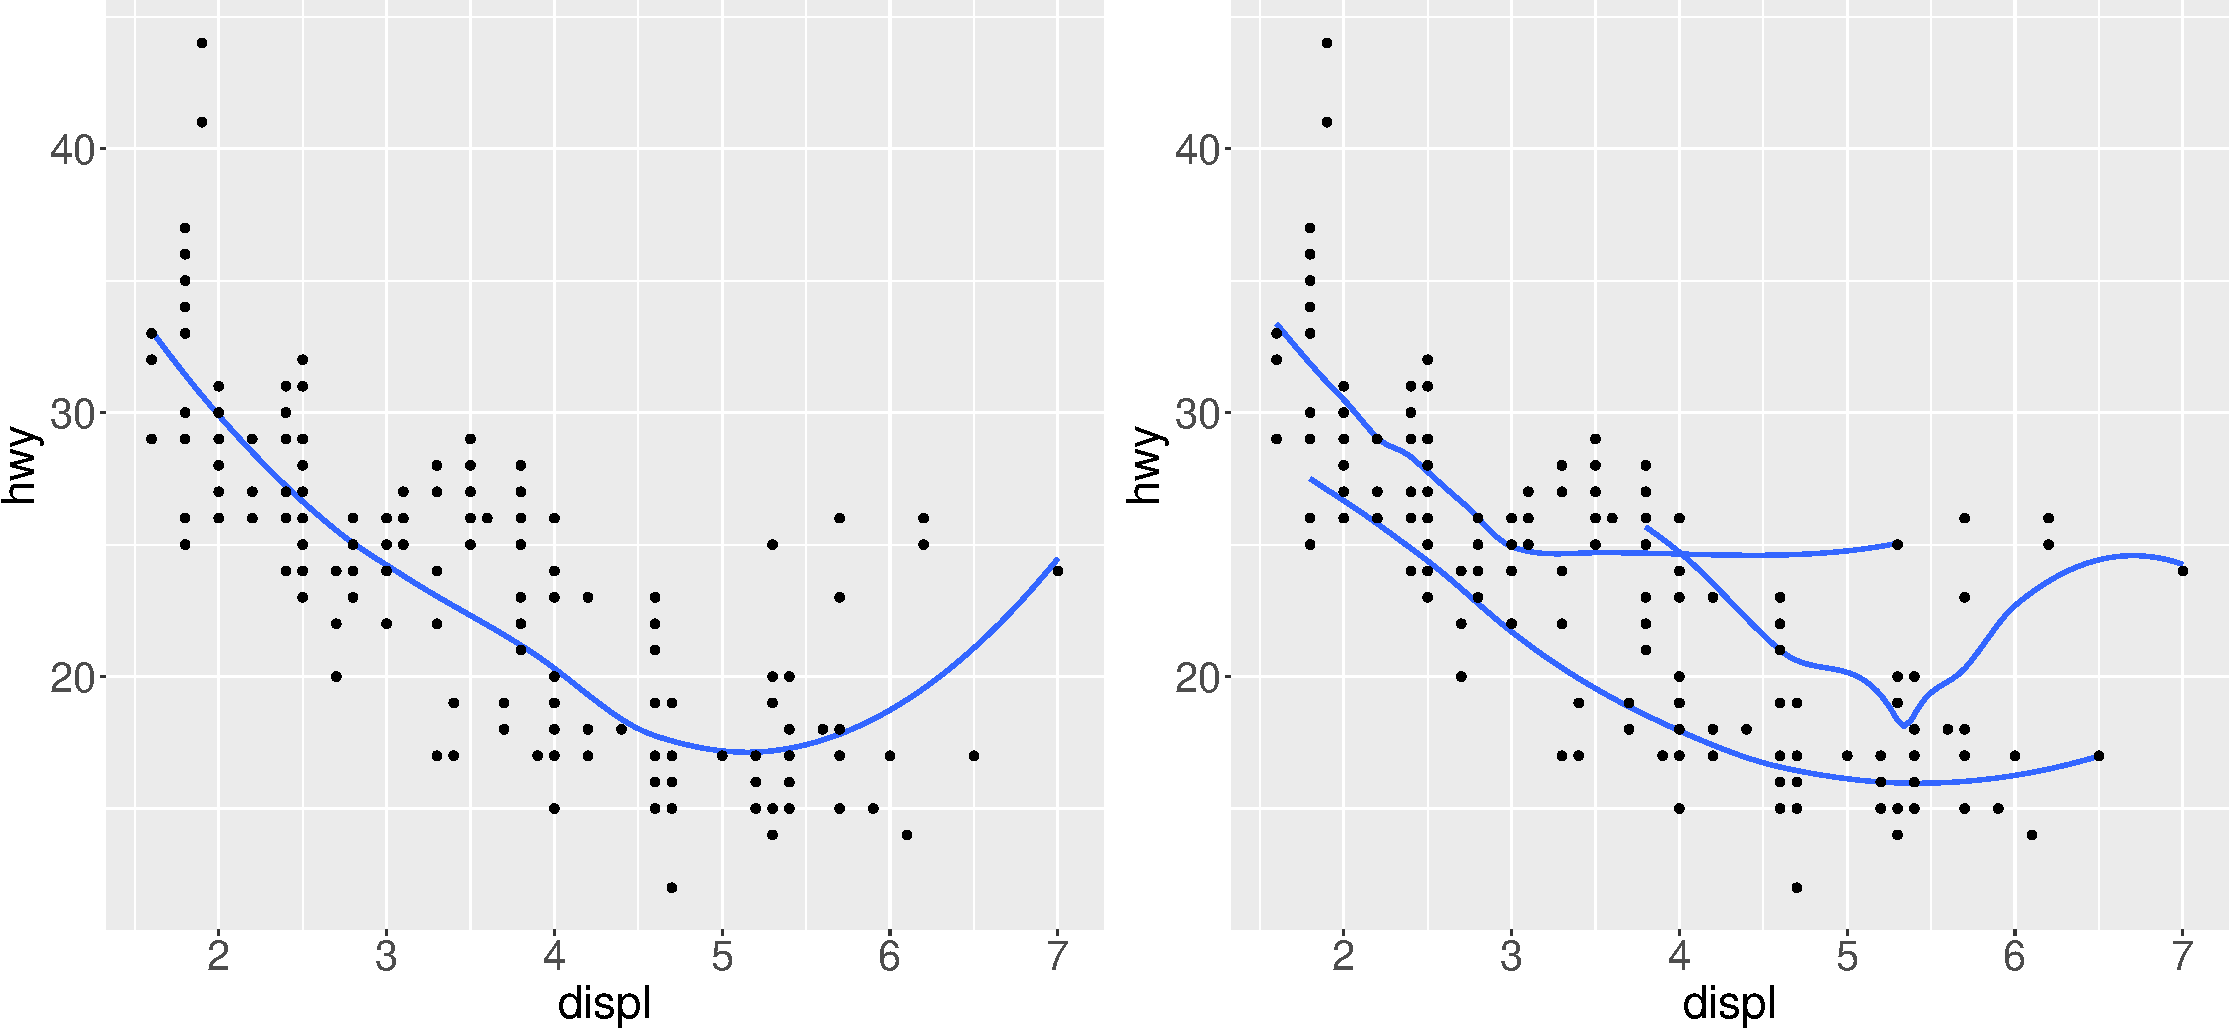
\includegraphics[height=150px]{data-visualization_files/figure-beamer/unnamed-chunk-82-1} \end{center}

\end{frame}

\begin{frame}[fragile]{Multiple geoms}
\protect\hypertarget{multiple-geoms-4}{}

\begin{itemize}
\item
  This, however, induces duplication in our code.
\item
  We built the same aesthetic mapping twice in each graph.
\item
  We can avoid this type of repetition by passing a set of mappings to
  \texttt{ggplot()}.
\item
  ggplot2 will treat these mappings as global mappings that apply to
  each geom in the graph.
\end{itemize}

\end{frame}

\begin{frame}[fragile]{Multiple geoms}
\protect\hypertarget{multiple-geoms-5}{}

These two chunks of code result in the same plot:

\begin{Shaded}
\begin{Highlighting}[]
\KeywordTok{ggplot}\NormalTok{(}\DataTypeTok{data =}\NormalTok{ mpg) }\OperatorTok{+}\StringTok{ }
\StringTok{  }\KeywordTok{geom_point}\NormalTok{(}\KeywordTok{aes}\NormalTok{(}\DataTypeTok{x =}\NormalTok{ displ, }\DataTypeTok{y =}\NormalTok{ hwy)) }\OperatorTok{+}
\StringTok{  }\KeywordTok{geom_smooth}\NormalTok{(}\KeywordTok{aes}\NormalTok{(}\DataTypeTok{x =}\NormalTok{ displ, }\DataTypeTok{y =}\NormalTok{ hwy))}
\end{Highlighting}
\end{Shaded}

\begin{Shaded}
\begin{Highlighting}[]
\KeywordTok{ggplot}\NormalTok{(}\DataTypeTok{data =}\NormalTok{ mpg, }\KeywordTok{aes}\NormalTok{(}\DataTypeTok{x =}\NormalTok{ displ, }\DataTypeTok{y =}\NormalTok{ hwy)) }\OperatorTok{+}\StringTok{ }
\StringTok{  }\KeywordTok{geom_point}\NormalTok{() }\OperatorTok{+}\StringTok{ }
\StringTok{  }\KeywordTok{geom_smooth}\NormalTok{()}
\end{Highlighting}
\end{Shaded}

\end{frame}

\begin{frame}{Multiple geoms}
\protect\hypertarget{multiple-geoms-6}{}

\begin{center}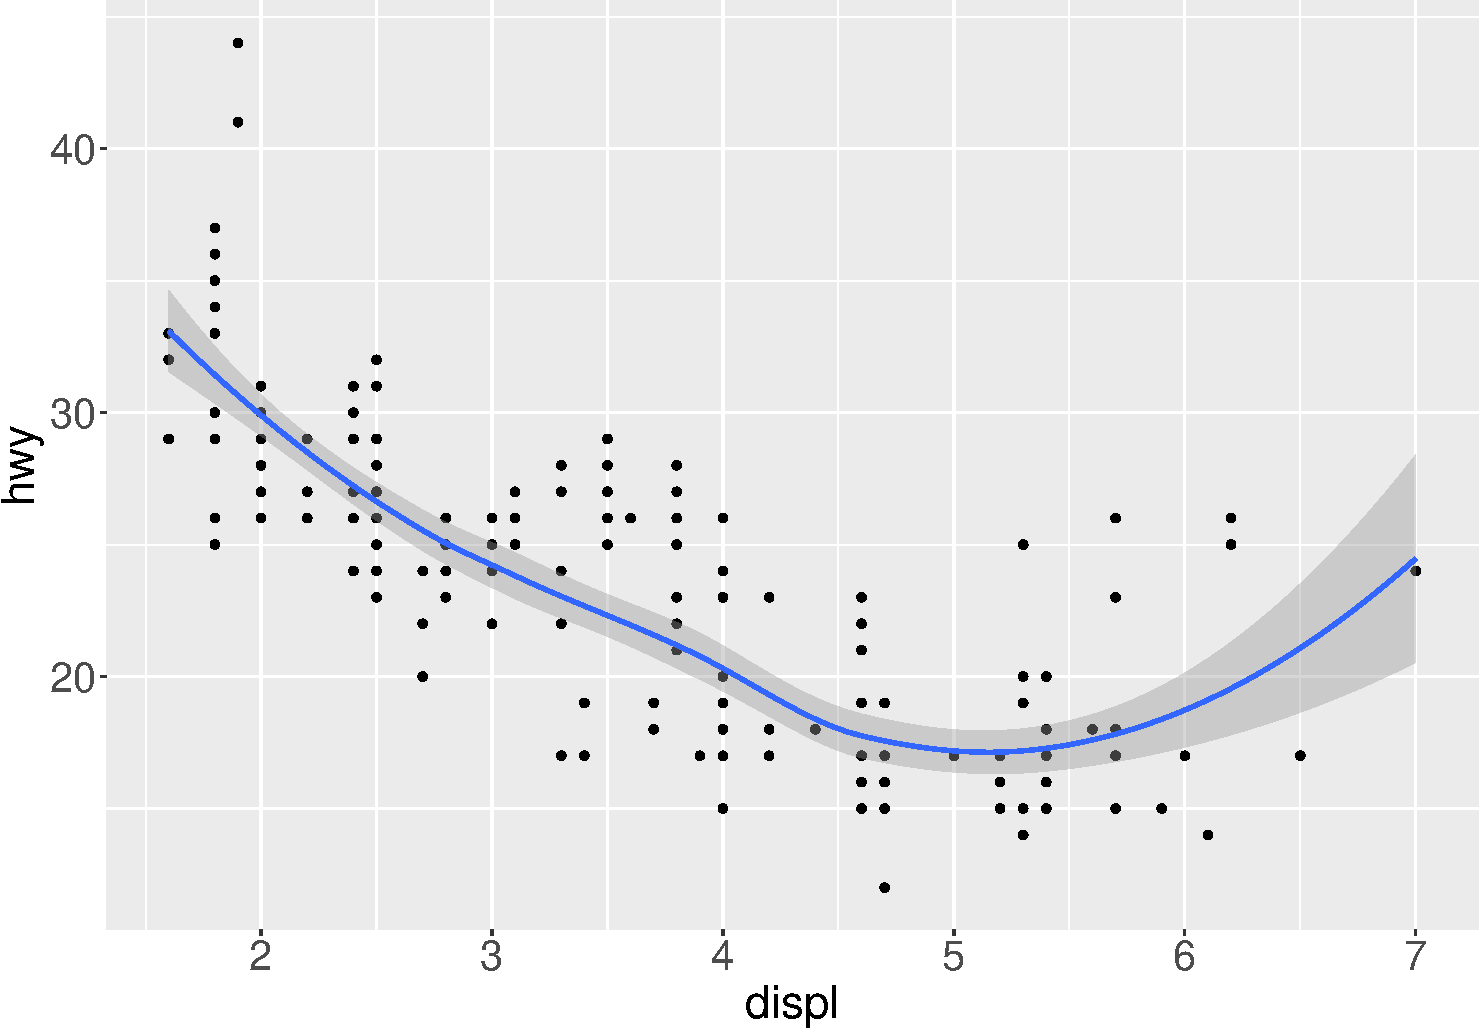
\includegraphics[height=200px]{data-visualization_files/figure-beamer/unnamed-chunk-85-1} \end{center}

\end{frame}

\begin{frame}{Multiple geoms}
\protect\hypertarget{multiple-geoms-7}{}

\begin{itemize}
\item
  If you place mappings in a geom function, ggplot2 will treat them as
  local mappings for that layer.
\item
  It will use these mappings to extend or overwrite the global mappings
  for that layer only.
\item
  This makes it possible to display different aesthetics in different
  layers.
\end{itemize}

\end{frame}

\begin{frame}[fragile]{Multiple geoms}
\protect\hypertarget{multiple-geoms-8}{}

\begin{Shaded}
\begin{Highlighting}[]
\KeywordTok{ggplot}\NormalTok{(}\DataTypeTok{data =}\NormalTok{ mpg, }\KeywordTok{aes}\NormalTok{(}\DataTypeTok{x =}\NormalTok{ displ, }\DataTypeTok{y =}\NormalTok{ hwy)) }\OperatorTok{+}\StringTok{ }
\StringTok{  }\KeywordTok{geom_smooth}\NormalTok{(}\KeywordTok{aes}\NormalTok{(}\DataTypeTok{color =}\NormalTok{ drv), }\DataTypeTok{se =} \OtherTok{FALSE}\NormalTok{) }\OperatorTok{+}
\StringTok{  }\KeywordTok{geom_point}\NormalTok{()}
\end{Highlighting}
\end{Shaded}

\end{frame}

\begin{frame}{Multiple geoms}
\protect\hypertarget{multiple-geoms-9}{}

\begin{center}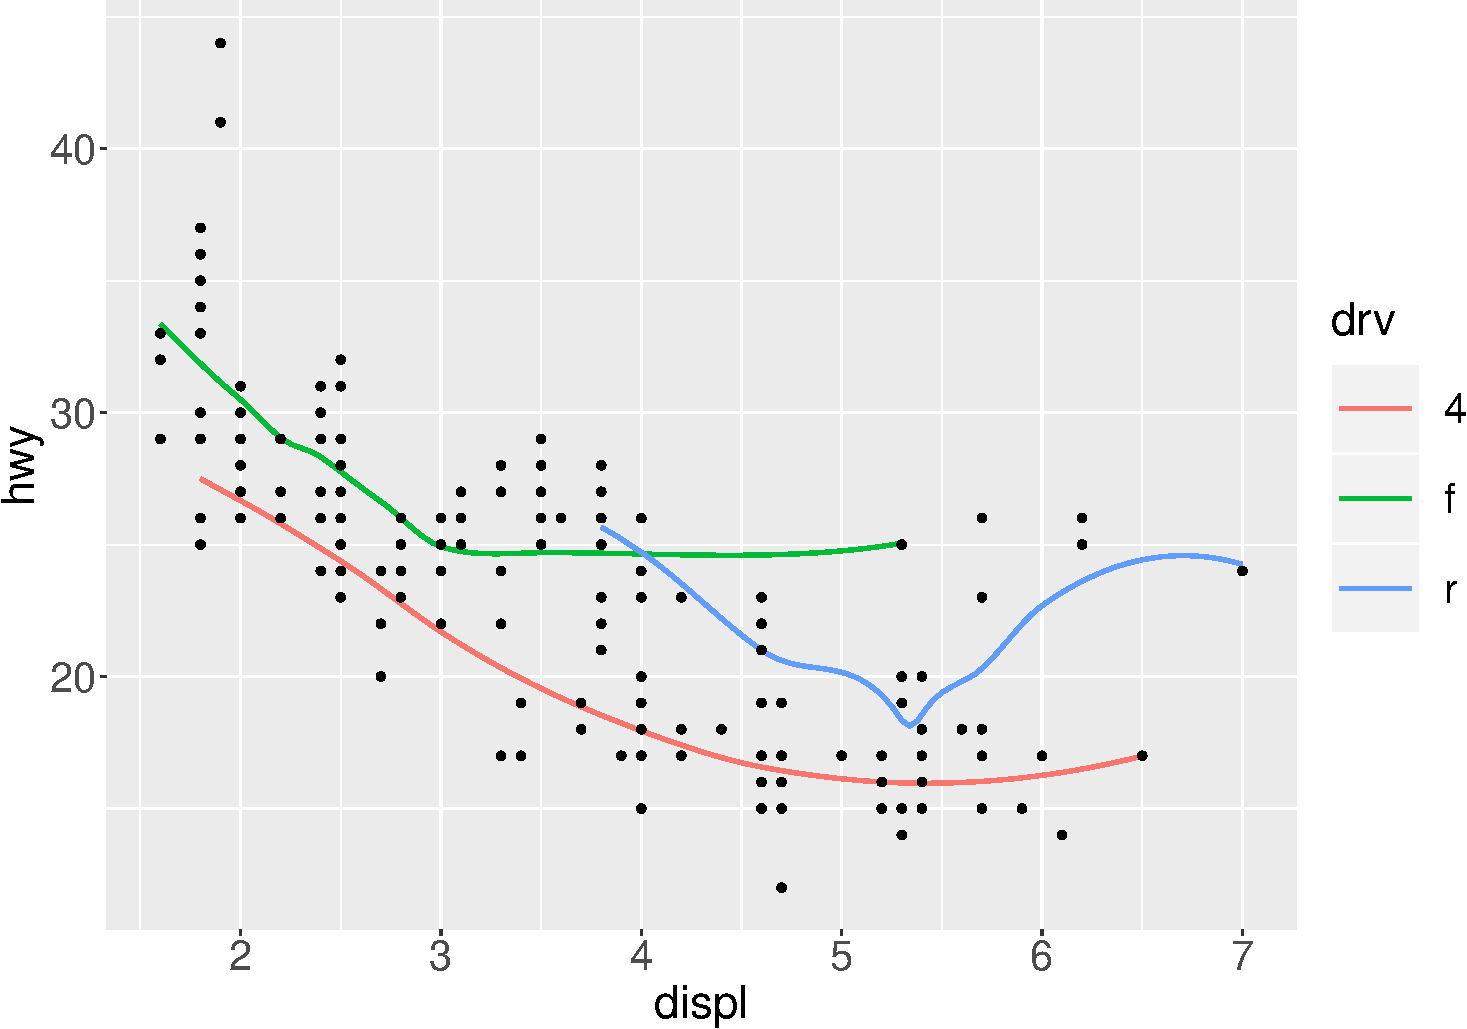
\includegraphics[height=200px]{data-visualization_files/figure-beamer/unnamed-chunk-87-1} \end{center}

\end{frame}

\begin{frame}[fragile]{Multiple geoms}
\protect\hypertarget{multiple-geoms-10}{}

\begin{Shaded}
\begin{Highlighting}[]
\KeywordTok{ggplot}\NormalTok{(}\DataTypeTok{data =}\NormalTok{ mpg, }
       \KeywordTok{aes}\NormalTok{(}\DataTypeTok{x =}\NormalTok{ displ, }\DataTypeTok{y =}\NormalTok{ hwy, }\DataTypeTok{color =}\NormalTok{ drv)) }\OperatorTok{+}\StringTok{ }
\StringTok{  }\KeywordTok{geom_smooth}\NormalTok{(}\DataTypeTok{se =} \OtherTok{FALSE}\NormalTok{) }\OperatorTok{+}
\StringTok{  }\KeywordTok{geom_point}\NormalTok{()}
\end{Highlighting}
\end{Shaded}

\end{frame}

\begin{frame}{Multiple geoms}
\protect\hypertarget{multiple-geoms-11}{}

\begin{center}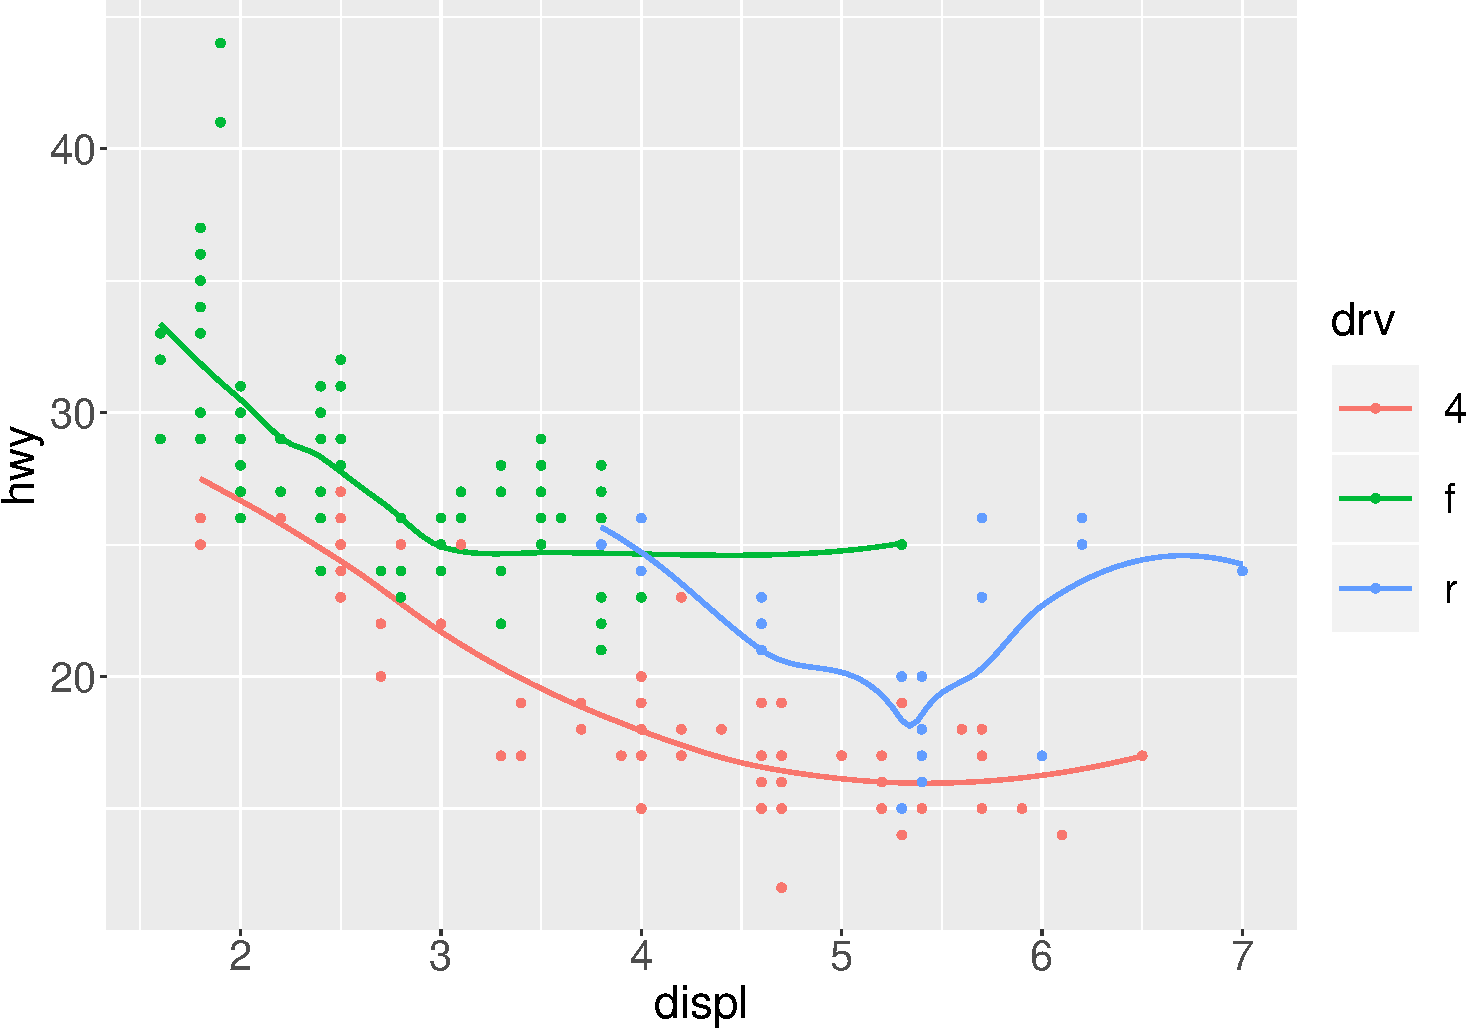
\includegraphics[height=200px]{data-visualization_files/figure-beamer/unnamed-chunk-89-1} \end{center}

\end{frame}

\begin{frame}[fragile]{Multiple geoms}
\protect\hypertarget{multiple-geoms-12}{}

\begin{Shaded}
\begin{Highlighting}[]
\KeywordTok{ggplot}\NormalTok{(}\DataTypeTok{data =}\NormalTok{ mpg, }\KeywordTok{aes}\NormalTok{(}\DataTypeTok{x =}\NormalTok{ displ, }\DataTypeTok{y =}\NormalTok{ hwy)) }\OperatorTok{+}
\StringTok{   }\KeywordTok{geom_smooth}\NormalTok{(}\KeywordTok{aes}\NormalTok{(}\DataTypeTok{linetype =}\NormalTok{ drv), }\DataTypeTok{se =} \OtherTok{FALSE}\NormalTok{) }\OperatorTok{+}
\StringTok{   }\KeywordTok{geom_point}\NormalTok{(}\KeywordTok{aes}\NormalTok{(}\DataTypeTok{color =}\NormalTok{ drv))}
\end{Highlighting}
\end{Shaded}

\end{frame}

\begin{frame}{Multiple geoms}
\protect\hypertarget{multiple-geoms-13}{}

\begin{center}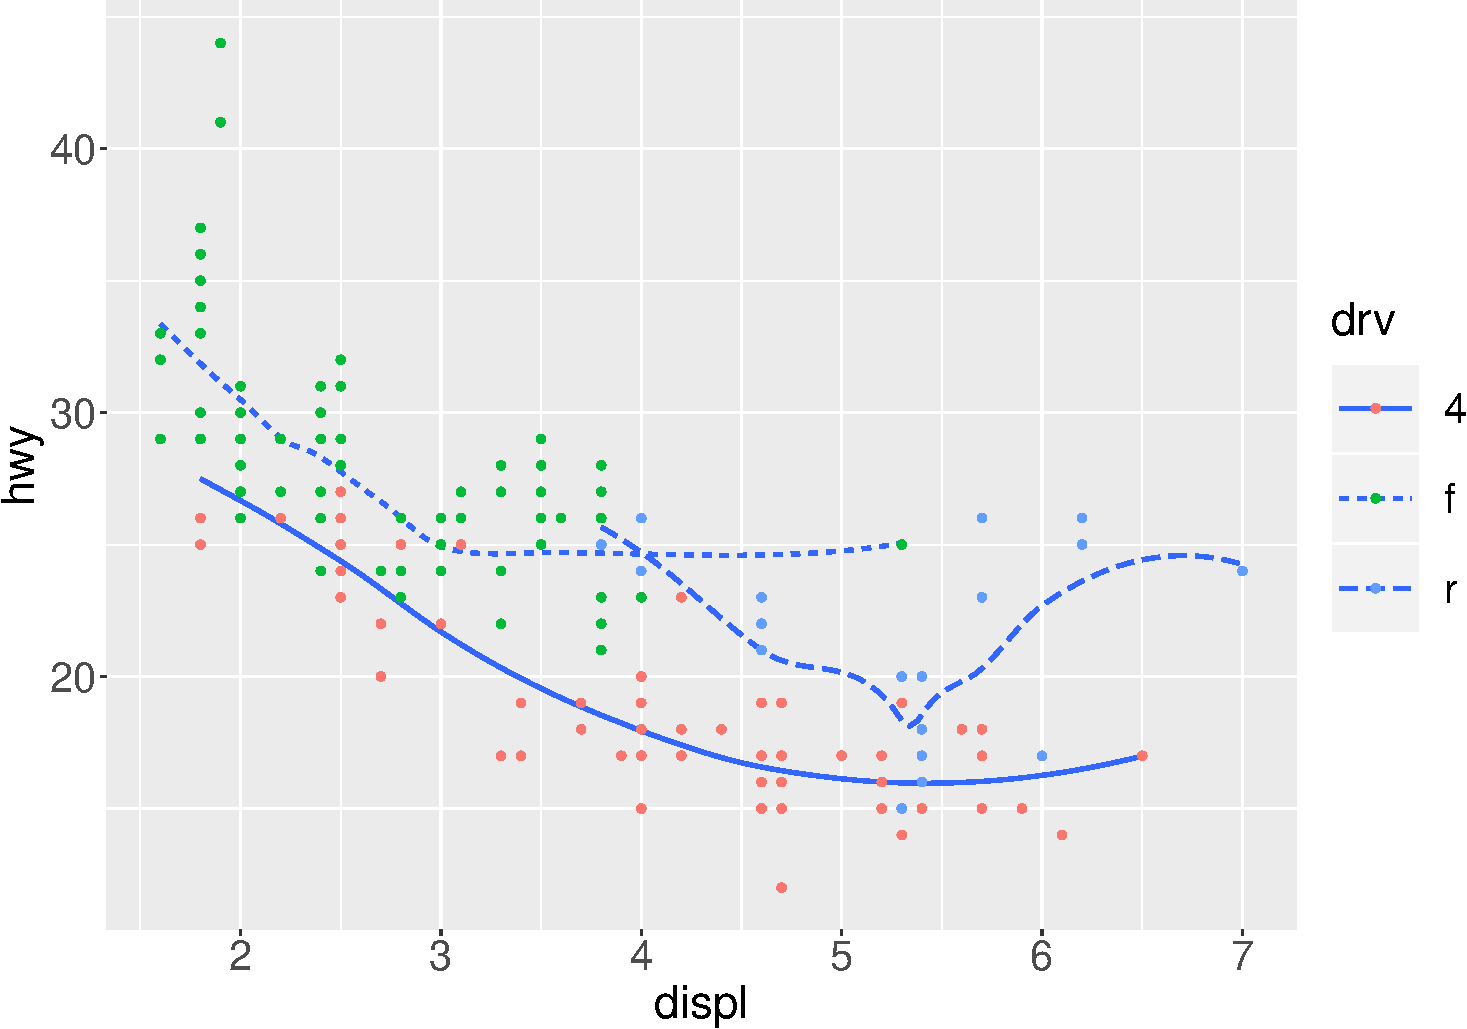
\includegraphics[height=200px]{data-visualization_files/figure-beamer/unnamed-chunk-91-1} \end{center}

\end{frame}

\begin{frame}[fragile]{Multiple geoms}
\protect\hypertarget{multiple-geoms-14}{}

\begin{Shaded}
\begin{Highlighting}[]
\KeywordTok{ggplot}\NormalTok{(}\DataTypeTok{data =}\NormalTok{ mpg, }\KeywordTok{aes}\NormalTok{(}\DataTypeTok{x =}\NormalTok{ displ, }\DataTypeTok{y =}\NormalTok{ hwy, }
                       \DataTypeTok{color =}\NormalTok{ drv)) }\OperatorTok{+}
\StringTok{  }\KeywordTok{geom_smooth}\NormalTok{(}\KeywordTok{aes}\NormalTok{(}\DataTypeTok{linetype =}\NormalTok{ drv), }\DataTypeTok{se =} \OtherTok{FALSE}\NormalTok{) }\OperatorTok{+}
\StringTok{  }\KeywordTok{geom_point}\NormalTok{()}
\end{Highlighting}
\end{Shaded}

\end{frame}

\begin{frame}{Multiple geoms}
\protect\hypertarget{multiple-geoms-15}{}

\begin{center}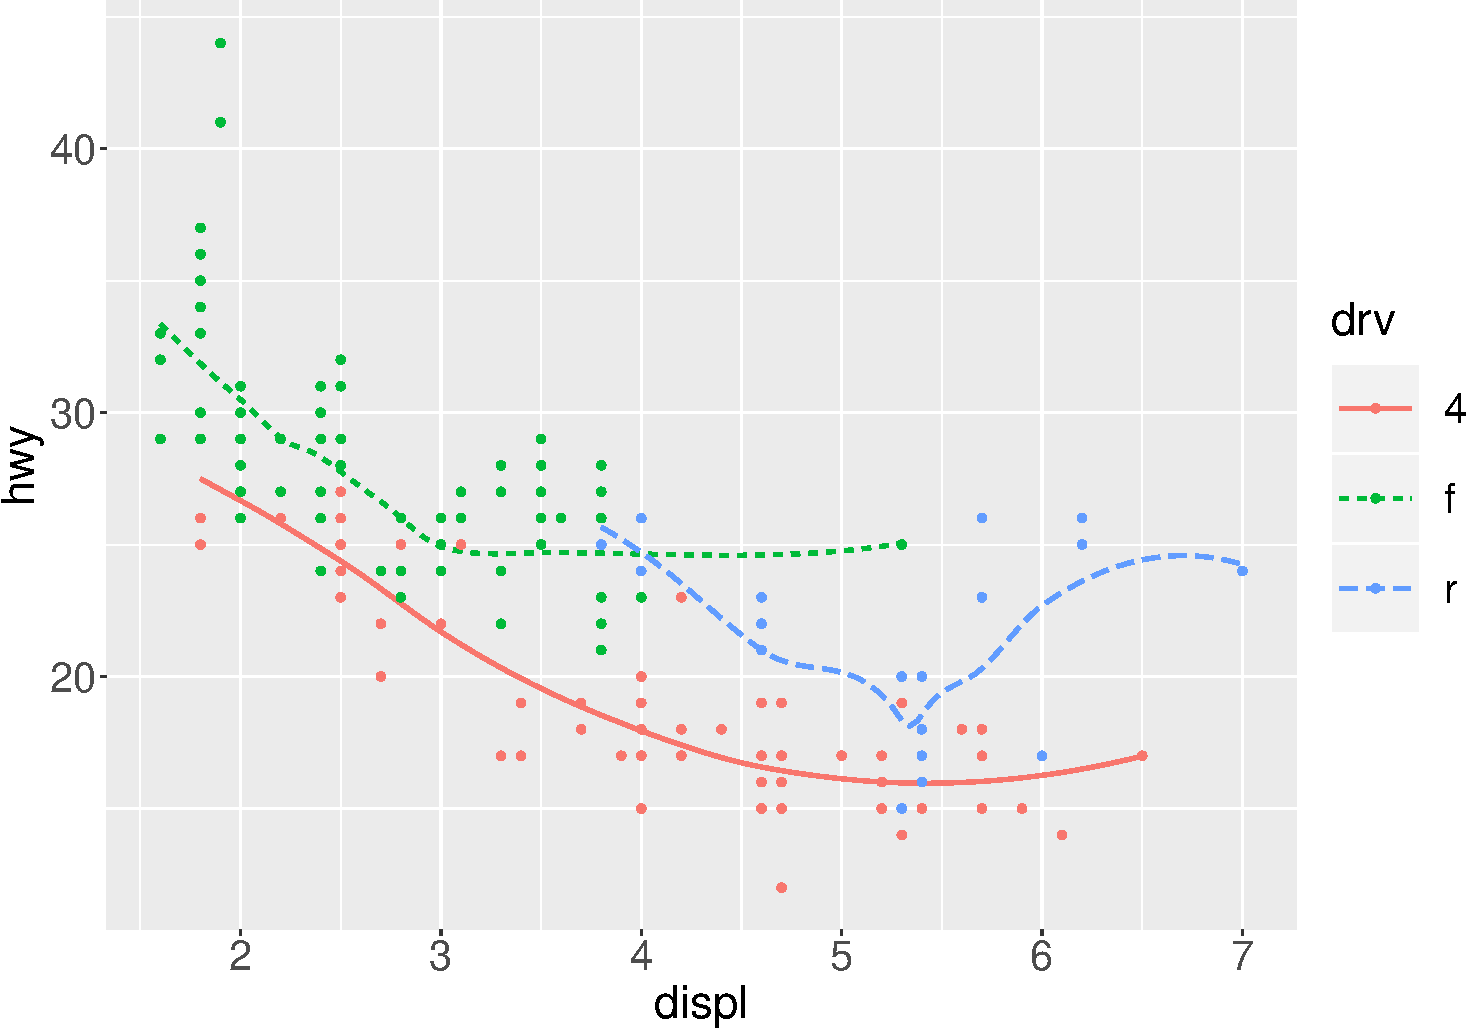
\includegraphics[height=200px]{data-visualization_files/figure-beamer/unnamed-chunk-93-1} \end{center}

\end{frame}

\begin{frame}[fragile]{Multiple geoms}
\protect\hypertarget{multiple-geoms-16}{}

\begin{Shaded}
\begin{Highlighting}[]
\KeywordTok{ggplot}\NormalTok{(}\DataTypeTok{data =}\NormalTok{ mpg, }\KeywordTok{aes}\NormalTok{(}\DataTypeTok{x =}\NormalTok{ displ, }\DataTypeTok{y =}\NormalTok{ hwy)) }\OperatorTok{+}\StringTok{ }
\StringTok{  }\KeywordTok{geom_point}\NormalTok{(}\KeywordTok{aes}\NormalTok{(}\DataTypeTok{color =}\NormalTok{ class)) }\OperatorTok{+}\StringTok{ }
\StringTok{  }\KeywordTok{geom_smooth}\NormalTok{()}
\end{Highlighting}
\end{Shaded}

\end{frame}

\begin{frame}{Multiple geoms}
\protect\hypertarget{multiple-geoms-17}{}

\begin{center}\includegraphics[height=200px]{data-visualization_files/figure-beamer/unnamed-chunk-95-1} \end{center}

\end{frame}

\begin{frame}[fragile]{Multiple geoms}
\protect\hypertarget{multiple-geoms-18}{}

\begin{Shaded}
\begin{Highlighting}[]
\KeywordTok{ggplot}\NormalTok{(}\DataTypeTok{data =}\NormalTok{ mpg, }\KeywordTok{aes}\NormalTok{(}\DataTypeTok{x =}\NormalTok{ displ, }\DataTypeTok{y =}\NormalTok{ hwy)) }\OperatorTok{+}\StringTok{ }
\StringTok{  }\KeywordTok{geom_smooth}\NormalTok{(}\KeywordTok{aes}\NormalTok{(}\DataTypeTok{linetype =}\NormalTok{ drv)) }\OperatorTok{+}
\StringTok{  }\KeywordTok{geom_point}\NormalTok{(}\KeywordTok{aes}\NormalTok{(}\DataTypeTok{color =}\NormalTok{ class))}
\end{Highlighting}
\end{Shaded}

\end{frame}

\begin{frame}{Multiple geoms}
\protect\hypertarget{multiple-geoms-19}{}

\begin{center}\includegraphics[height=200px]{data-visualization_files/figure-beamer/unnamed-chunk-97-1} \end{center}

\end{frame}

\begin{frame}[fragile]{Multiple geoms}
\protect\hypertarget{multiple-geoms-20}{}

\begin{Shaded}
\begin{Highlighting}[]
\KeywordTok{ggplot}\NormalTok{(}\DataTypeTok{data =}\NormalTok{ mpg, }\KeywordTok{aes}\NormalTok{(}\DataTypeTok{x =}\NormalTok{ displ, }\DataTypeTok{y =}\NormalTok{ hwy)) }\OperatorTok{+}\StringTok{ }
\StringTok{  }\KeywordTok{geom_smooth}\NormalTok{(}\KeywordTok{aes}\NormalTok{(}\DataTypeTok{linetype =}\NormalTok{ drv), }\DataTypeTok{se =} \OtherTok{FALSE}\NormalTok{) }\OperatorTok{+}
\StringTok{  }\KeywordTok{geom_point}\NormalTok{(}\KeywordTok{aes}\NormalTok{(}\DataTypeTok{color =}\NormalTok{ class))}
\end{Highlighting}
\end{Shaded}

\end{frame}

\begin{frame}{Multiple geoms}
\protect\hypertarget{multiple-geoms-21}{}

\begin{center}\includegraphics[height=200px]{data-visualization_files/figure-beamer/unnamed-chunk-99-1} \end{center}

\end{frame}

\begin{frame}[fragile]{Multiple geoms}
\protect\hypertarget{multiple-geoms-22}{}

We can also overlap geoms in grids:

\begin{Shaded}
\begin{Highlighting}[]
\KeywordTok{ggplot}\NormalTok{(}\DataTypeTok{data =}\NormalTok{ mpg, }\KeywordTok{aes}\NormalTok{(}\DataTypeTok{x =}\NormalTok{ displ, }\DataTypeTok{y =}\NormalTok{ hwy)) }\OperatorTok{+}\StringTok{ }
\StringTok{  }\KeywordTok{geom_smooth}\NormalTok{(}\DataTypeTok{se =} \OtherTok{FALSE}\NormalTok{) }\OperatorTok{+}\StringTok{ }
\StringTok{  }\KeywordTok{geom_point}\NormalTok{() }\OperatorTok{+}\StringTok{ }
\StringTok{  }\KeywordTok{facet_wrap}\NormalTok{(}\OperatorTok{~}\NormalTok{class, }\DataTypeTok{nrow =} \DecValTok{2}\NormalTok{)}
\end{Highlighting}
\end{Shaded}

\end{frame}

\begin{frame}{Multiple geoms}
\protect\hypertarget{multiple-geoms-23}{}

\begin{center}\includegraphics[height=200px]{data-visualization_files/figure-beamer/unnamed-chunk-101-1} \end{center}

\end{frame}

\begin{frame}[fragile]{Multiple geoms}
\protect\hypertarget{multiple-geoms-24}{}

\begin{Shaded}
\begin{Highlighting}[]
\KeywordTok{ggplot}\NormalTok{(}\DataTypeTok{data =}\NormalTok{ mpg, }\KeywordTok{aes}\NormalTok{(}\DataTypeTok{x =}\NormalTok{ displ, }\DataTypeTok{y =}\NormalTok{ hwy)) }\OperatorTok{+}\StringTok{ }
\StringTok{  }\KeywordTok{geom_point}\NormalTok{() }\OperatorTok{+}\StringTok{ }
\StringTok{  }\KeywordTok{geom_smooth}\NormalTok{(}\DataTypeTok{method =} \StringTok{"lm"}\NormalTok{, }\DataTypeTok{se =} \OtherTok{FALSE}\NormalTok{) }\OperatorTok{+}\StringTok{ }
\StringTok{  }\KeywordTok{facet_wrap}\NormalTok{(}\OperatorTok{~}\NormalTok{class, }\DataTypeTok{nrow =} \DecValTok{2}\NormalTok{)}
\end{Highlighting}
\end{Shaded}

\end{frame}

\begin{frame}{Multiple geoms}
\protect\hypertarget{multiple-geoms-25}{}

\begin{center}\includegraphics[height=200px]{data-visualization_files/figure-beamer/unnamed-chunk-103-1} \end{center}

\end{frame}

\begin{frame}{Multiple geoms}
\protect\hypertarget{multiple-geoms-26}{}

\begin{itemize}
\tightlist
\item
  You can use the same logic to specify a different dataset for each
  layer.
\end{itemize}

\end{frame}

\begin{frame}[fragile]{Multiple geoms}
\protect\hypertarget{multiple-geoms-27}{}

\begin{Shaded}
\begin{Highlighting}[]
\NormalTok{subcompact <-}\StringTok{ }\KeywordTok{subset}\NormalTok{(mpg, class }\OperatorTok{==}\StringTok{ "subcompact"}\NormalTok{)}

\KeywordTok{ggplot}\NormalTok{(}\DataTypeTok{data =}\NormalTok{ mpg, }\KeywordTok{aes}\NormalTok{(}\DataTypeTok{x =}\NormalTok{ displ, }\DataTypeTok{y =}\NormalTok{ hwy)) }\OperatorTok{+}
\StringTok{  }\KeywordTok{geom_point}\NormalTok{(}\KeywordTok{aes}\NormalTok{(}\DataTypeTok{color =}\NormalTok{ class)) }\OperatorTok{+}
\StringTok{  }\KeywordTok{geom_smooth}\NormalTok{(}\DataTypeTok{data =}\NormalTok{ subcompact, }\DataTypeTok{se =} \OtherTok{FALSE}\NormalTok{, }
              \DataTypeTok{method =} \StringTok{"lm"}\NormalTok{)}
\end{Highlighting}
\end{Shaded}

\begin{itemize}
\item
  The straight line displays just a subset of the mpg dataset, the
  subcompact cars.
\item
  The local data argument in geom\_smooth() overrides the global data
  argument in \texttt{ggplot()} for that layer only.
\end{itemize}

\end{frame}

\begin{frame}{Multiple geoms}
\protect\hypertarget{multiple-geoms-28}{}

\begin{center}\includegraphics[height=300px]{data-visualization_files/figure-beamer/unnamed-chunk-105-1} \end{center}

\end{frame}

\begin{frame}[fragile]{Multiple geoms}
\protect\hypertarget{multiple-geoms-29}{}

\begin{Shaded}
\begin{Highlighting}[]
\NormalTok{subcompact <-}\StringTok{ }\KeywordTok{subset}\NormalTok{(mpg, class }\OperatorTok{==}\StringTok{ "subcompact"}\NormalTok{)}
\NormalTok{two_seater <-}\StringTok{ }\KeywordTok{subset}\NormalTok{(mpg, class }\OperatorTok{==}\StringTok{ "2seater"}\NormalTok{)}

\KeywordTok{ggplot}\NormalTok{(}\DataTypeTok{data =}\NormalTok{ mpg, }\KeywordTok{aes}\NormalTok{(}\DataTypeTok{x =}\NormalTok{ displ, }\DataTypeTok{y =}\NormalTok{ hwy)) }\OperatorTok{+}
\StringTok{  }\KeywordTok{geom_point}\NormalTok{(}\KeywordTok{aes}\NormalTok{(}\DataTypeTok{color =}\NormalTok{ class)) }\OperatorTok{+}
\StringTok{  }\KeywordTok{geom_smooth}\NormalTok{(}\DataTypeTok{data =}\NormalTok{ subcompact, }\DataTypeTok{se =} \OtherTok{FALSE}\NormalTok{,}
              \DataTypeTok{method =} \StringTok{"lm"}\NormalTok{) }\OperatorTok{+}
\StringTok{  }\KeywordTok{geom_smooth}\NormalTok{(}\DataTypeTok{data =}\NormalTok{ two_seater, }\DataTypeTok{se =} \OtherTok{FALSE}\NormalTok{,}
              \DataTypeTok{method =} \StringTok{"lm"}\NormalTok{)}
\end{Highlighting}
\end{Shaded}

\end{frame}

\begin{frame}{Multiple geoms}
\protect\hypertarget{multiple-geoms-30}{}

\begin{center}\includegraphics[height=200px]{data-visualization_files/figure-beamer/unnamed-chunk-107-1} \end{center}

\end{frame}

\begin{frame}[fragile]{Multiple geoms}
\protect\hypertarget{multiple-geoms-31}{}

\begin{Shaded}
\begin{Highlighting}[]
\KeywordTok{ggplot}\NormalTok{(}\DataTypeTok{data =}\NormalTok{ mpg, }\KeywordTok{aes}\NormalTok{(}\DataTypeTok{x =}\NormalTok{ displ, }\DataTypeTok{y =}\NormalTok{ hwy)) }\OperatorTok{+}
\StringTok{       }\KeywordTok{geom_point}\NormalTok{(}\KeywordTok{aes}\NormalTok{(}\DataTypeTok{color =}\NormalTok{ class)) }\OperatorTok{+}
\StringTok{       }\KeywordTok{geom_smooth}\NormalTok{(}
         \DataTypeTok{data =} \KeywordTok{subset}\NormalTok{(mpg, class }\OperatorTok{!=}\StringTok{ "2seater"}\NormalTok{),}
         \DataTypeTok{se =} \OtherTok{FALSE}\NormalTok{,}
         \DataTypeTok{method =} \StringTok{"lm"}\NormalTok{)}
\end{Highlighting}
\end{Shaded}

\end{frame}

\begin{frame}{Multiple geoms}
\protect\hypertarget{multiple-geoms-32}{}

\begin{center}\includegraphics[height=300px]{data-visualization_files/figure-beamer/unnamed-chunk-109-1} \end{center}

\end{frame}

\begin{frame}[fragile]{Multiple geoms}
\protect\hypertarget{multiple-geoms-33}{}

\begin{Shaded}
\begin{Highlighting}[]
\NormalTok{corvette <-}\StringTok{ }\KeywordTok{subset}\NormalTok{(mpg, model }\OperatorTok{==}\StringTok{ "corvette"}\NormalTok{)}
\NormalTok{not_corvette <-}\StringTok{ }\KeywordTok{subset}\NormalTok{(mpg, model }\OperatorTok{!=}\StringTok{ "corvette"}\NormalTok{)}

\KeywordTok{ggplot}\NormalTok{(}\DataTypeTok{mapping =} \KeywordTok{aes}\NormalTok{(}\DataTypeTok{x =}\NormalTok{ displ, }\DataTypeTok{y =}\NormalTok{ hwy)) }\OperatorTok{+}\StringTok{ }
\StringTok{  }\KeywordTok{geom_point}\NormalTok{(}\DataTypeTok{data =}\NormalTok{ not_corvette) }\OperatorTok{+}\StringTok{ }
\StringTok{  }\KeywordTok{geom_point}\NormalTok{(}\DataTypeTok{data =}\NormalTok{ corvette,  }\DataTypeTok{color =} \StringTok{"Red"}\NormalTok{)}
\end{Highlighting}
\end{Shaded}

\end{frame}

\begin{frame}{Multiple geoms}
\protect\hypertarget{multiple-geoms-34}{}

\begin{center}\includegraphics[height=300px]{data-visualization_files/figure-beamer/unnamed-chunk-111-1} \end{center}

\end{frame}

\begin{frame}[fragile]{Labels}
\protect\hypertarget{labels}{}

We can add labels to a graph with the \texttt{labs()} function:

\begin{Shaded}
\begin{Highlighting}[]
\KeywordTok{ggplot}\NormalTok{(mpg, }\KeywordTok{aes}\NormalTok{(displ, hwy)) }\OperatorTok{+}
\StringTok{  }\KeywordTok{geom_point}\NormalTok{(}\KeywordTok{aes}\NormalTok{(}\DataTypeTok{color =}\NormalTok{ class)) }\OperatorTok{+}
\StringTok{  }\KeywordTok{geom_smooth}\NormalTok{(}\DataTypeTok{se =} \OtherTok{FALSE}\NormalTok{) }\OperatorTok{+}
\StringTok{  }\KeywordTok{labs}\NormalTok{(}
    \DataTypeTok{title =} \StringTok{"Efficiency decreases with engine size"}\NormalTok{)}
\end{Highlighting}
\end{Shaded}

\end{frame}

\begin{frame}{Labels}
\protect\hypertarget{labels-1}{}

\begin{center}\includegraphics[height=200px]{data-visualization_files/figure-beamer/unnamed-chunk-113-1} \end{center}

\end{frame}

\begin{frame}[fragile]{Labels}
\protect\hypertarget{labels-2}{}

The \texttt{labs()} function can also be used to add a subtitle and/or a
caption:

\begin{Shaded}
\begin{Highlighting}[]
\KeywordTok{ggplot}\NormalTok{(mpg, }\KeywordTok{aes}\NormalTok{(displ, hwy)) }\OperatorTok{+}
\StringTok{  }\KeywordTok{geom_point}\NormalTok{(}\KeywordTok{aes}\NormalTok{(}\DataTypeTok{color =}\NormalTok{ class)) }\OperatorTok{+}
\StringTok{  }\KeywordTok{geom_smooth}\NormalTok{(}\DataTypeTok{se =} \OtherTok{FALSE}\NormalTok{) }\OperatorTok{+}
\StringTok{  }\KeywordTok{labs}\NormalTok{(}
    \DataTypeTok{title =} \StringTok{"Efficiency decreases with engine size"}\NormalTok{,}
    \DataTypeTok{subtitle =} \StringTok{"Two-seaters are an exception"}\NormalTok{,}
    \DataTypeTok{caption =} \StringTok{"Data from fueleconomy.gov"}
\NormalTok{  )}
\end{Highlighting}
\end{Shaded}

\end{frame}

\begin{frame}{Labels}
\protect\hypertarget{labels-3}{}

\begin{center}\includegraphics[height=200px]{data-visualization_files/figure-beamer/unnamed-chunk-115-1} \end{center}

\end{frame}

\begin{frame}{Labels}
\protect\hypertarget{labels-4}{}

\begin{itemize}
\item
  You can also use labs() to replace the axis and legend titles.
\item
  It's usually a good idea to replace short variable names with more
  detailed descriptions, and to include the units.
\end{itemize}

\end{frame}

\begin{frame}[fragile]{Labels}
\protect\hypertarget{labels-5}{}

\begin{Shaded}
\begin{Highlighting}[]
\KeywordTok{ggplot}\NormalTok{(mpg, }\KeywordTok{aes}\NormalTok{(displ, hwy)) }\OperatorTok{+}
\StringTok{  }\KeywordTok{geom_point}\NormalTok{(}\KeywordTok{aes}\NormalTok{(}\DataTypeTok{colour =}\NormalTok{ class)) }\OperatorTok{+}
\StringTok{  }\KeywordTok{geom_smooth}\NormalTok{(}\DataTypeTok{se =} \OtherTok{FALSE}\NormalTok{) }\OperatorTok{+}
\StringTok{  }\KeywordTok{labs}\NormalTok{(}
    \DataTypeTok{x =} \StringTok{"Engine displacement (L)"}\NormalTok{,}
    \DataTypeTok{y =} \StringTok{"Highway fuel economy (mpg)"}\NormalTok{,}
    \DataTypeTok{colour =} \StringTok{"Car type"}
\end{Highlighting}
\end{Shaded}

\end{frame}

\begin{frame}{Labels}
\protect\hypertarget{labels-6}{}

\begin{center}\includegraphics[height=200px]{data-visualization_files/figure-beamer/unnamed-chunk-117-1} \end{center}

\end{frame}

\begin{frame}[fragile]{Labels}
\protect\hypertarget{labels-7}{}

It's possible to use mathematical equations instead of text strings:

\begin{Shaded}
\begin{Highlighting}[]
\NormalTok{df <-}\StringTok{ }\KeywordTok{tibble}\NormalTok{(}
  \DataTypeTok{x =} \KeywordTok{runif}\NormalTok{(}\DecValTok{10}\NormalTok{),}
  \DataTypeTok{y =} \KeywordTok{runif}\NormalTok{(}\DecValTok{10}\NormalTok{))}

\KeywordTok{ggplot}\NormalTok{(df, }\KeywordTok{aes}\NormalTok{(x, y)) }\OperatorTok{+}
\StringTok{  }\KeywordTok{geom_point}\NormalTok{() }\OperatorTok{+}
\StringTok{  }\KeywordTok{labs}\NormalTok{(}
    \DataTypeTok{x =} \KeywordTok{quote}\NormalTok{(}\KeywordTok{sum}\NormalTok{(x[i] }\OperatorTok{^}\StringTok{ }\DecValTok{2}\NormalTok{, i }\OperatorTok{==}\StringTok{ }\DecValTok{1}\NormalTok{, n)),}
    \DataTypeTok{y =} \KeywordTok{quote}\NormalTok{(alpha }\OperatorTok{+}\StringTok{ }\NormalTok{beta }\OperatorTok{+}\StringTok{ }\KeywordTok{frac}\NormalTok{(delta, theta))}
\NormalTok{  )}
\end{Highlighting}
\end{Shaded}

\end{frame}

\begin{frame}{Labels}
\protect\hypertarget{labels-8}{}

\begin{center}\includegraphics[height=200px]{data-visualization_files/figure-beamer/unnamed-chunk-119-1} \end{center}

\end{frame}

\begin{frame}[fragile]{Labels}
\protect\hypertarget{labels-9}{}

To learn more about the mathematical syntax available see:

\begin{Shaded}
\begin{Highlighting}[]
\NormalTok{?plotmath}
\end{Highlighting}
\end{Shaded}

\end{frame}

\begin{frame}{The \texttt{diamonds} dataset}
\protect\hypertarget{the-diamonds-dataset}{}

\begin{itemize}
\item
  Diamonds is a dataset included in the ggplot2 package.
\item
  Contains attributes of almost 54000 diamonds.
\item
  The variables include price, carat, quality of the cut, color and
  clarity
\end{itemize}

\end{frame}

\begin{frame}[fragile]{Bar charts}
\protect\hypertarget{bar-charts}{}

\begin{Shaded}
\begin{Highlighting}[]
\KeywordTok{ggplot}\NormalTok{(}\DataTypeTok{data =}\NormalTok{ diamonds) }\OperatorTok{+}\StringTok{ }
\StringTok{  }\KeywordTok{geom_bar}\NormalTok{(}\KeywordTok{aes}\NormalTok{(}\DataTypeTok{x =}\NormalTok{ cut))}
\end{Highlighting}
\end{Shaded}

\begin{center}\includegraphics[height=150px]{data-visualization_files/figure-beamer/unnamed-chunk-121-1} \end{center}

\end{frame}

\begin{frame}{Statistical transformations}
\protect\hypertarget{statistical-transformations}{}

\begin{itemize}
\item
  On the y-axis, bar charts displays counts.
\item
  But counts are not a variable in diamonds dataset!
\item
  Many graphs, like scatterplots, plot the raw values the dataset.
\item
  Other graphs, like bar charts, calculate new values to plot.
\item
  The algorithm used to calculate new values for a graph is called a
  \textbf{stat}, short for statistical transformation.
\end{itemize}

\end{frame}

\begin{frame}{Statistical transformations}
\protect\hypertarget{statistical-transformations-1}{}

\begin{itemize}
\item
  Bar charts, histograms, and frequency polygons bin your data and then
  plot bin counts.
\item
  Smoothers fit a model to your data and then plot predictions from the
  model.
\item
  Boxplots compute summary statistics and then display them on specially
  formatted box.
\end{itemize}

\end{frame}

\begin{frame}{Statistical transformations}
\protect\hypertarget{statistical-transformations-2}{}

\includegraphics[width=3.125in,height=\textheight]{figures/st1.png}

\end{frame}

\begin{frame}{Statistical transformations}
\protect\hypertarget{statistical-transformations-3}{}

\includegraphics[width=4.16667in,height=\textheight]{figures/st2.png}

\end{frame}

\begin{frame}[fragile]{Statistical transformations}
\protect\hypertarget{statistical-transformations-4}{}

\begin{itemize}
\item
  You can learn which stat a geom function uses by inspecting the
  default value of the \texttt{stat} argument.
\item
  For example, with \texttt{?geom\_bar} we learn that the default
  \texttt{stat} of \texttt{geom\_bar()} is \texttt{count}.
\item
  This means that \texttt{geom\_bar()} uses \texttt{stat\_count()} as
  the default statistical transformation.
\item
  You can generally use geoms and stats interchangeably.
\item
  For example, you can recreate the previous plot using
  \texttt{stat\_count()} instead of \texttt{geom\_bar()}.
\end{itemize}

\end{frame}

\begin{frame}[fragile]{Statistical transformations}
\protect\hypertarget{statistical-transformations-5}{}

\begin{Shaded}
\begin{Highlighting}[]
\KeywordTok{ggplot}\NormalTok{(}\DataTypeTok{data =}\NormalTok{ diamonds) }\OperatorTok{+}\StringTok{ }
\StringTok{  }\KeywordTok{stat_count}\NormalTok{(}\KeywordTok{aes}\NormalTok{(}\DataTypeTok{x =}\NormalTok{ cut))}
\end{Highlighting}
\end{Shaded}

\begin{center}\includegraphics[height=150px]{data-visualization_files/figure-beamer/unnamed-chunk-122-1} \end{center}

\end{frame}

\begin{frame}[fragile]{Statistical transformations}
\protect\hypertarget{statistical-transformations-6}{}

This works because:

\begin{itemize}
\item
  Every geom has a default stat, and every stat has a default geom.
\item
  The default \texttt{stat} of \texttt{geom\_bar()} is \texttt{count}.
\item
  The default \texttt{geom} of \texttt{stat\_count()} is \texttt{bar}.
\end{itemize}

\end{frame}

\begin{frame}[fragile]{Overwrithing the default stat}
\protect\hypertarget{overwrithing-the-default-stat}{}

What if we want a bar chart that plot data as is?

\begin{itemize}
\tightlist
\item
  We may have a column with column heights.
\item
  In that case, we need to change the default statistical
  transformation.
\end{itemize}

\begin{Shaded}
\begin{Highlighting}[]
\NormalTok{tib <-}\StringTok{ }\KeywordTok{tribble}\NormalTok{(}
  \OperatorTok{~}\NormalTok{cut,         }\OperatorTok{~}\NormalTok{freq,}
  \StringTok{"Fair"}\NormalTok{,       }\DecValTok{1610}\NormalTok{,}
  \StringTok{"Good"}\NormalTok{,       }\DecValTok{4906}\NormalTok{,}
  \StringTok{"Very Good"}\NormalTok{,  }\DecValTok{12082}\NormalTok{,}
  \StringTok{"Premium"}\NormalTok{,    }\DecValTok{13791}\NormalTok{,}
  \StringTok{"Ideal"}\NormalTok{,      }\DecValTok{21551}
\NormalTok{)}
\end{Highlighting}
\end{Shaded}

\end{frame}

\begin{frame}[fragile]{Overriding the default stat}
\protect\hypertarget{overriding-the-default-stat}{}

\begin{Shaded}
\begin{Highlighting}[]
\KeywordTok{ggplot}\NormalTok{(}\DataTypeTok{data =}\NormalTok{ tib) }\OperatorTok{+}
\StringTok{  }\KeywordTok{geom_bar}\NormalTok{(}\KeywordTok{aes}\NormalTok{(}\DataTypeTok{x =}\NormalTok{ cut, }\DataTypeTok{y =}\NormalTok{ freq),}
    \DataTypeTok{stat =} \StringTok{"identity"}\NormalTok{)}
\end{Highlighting}
\end{Shaded}

\begin{center}\includegraphics[height=150px]{data-visualization_files/figure-beamer/unnamed-chunk-124-1} \end{center}

\end{frame}

\begin{frame}[fragile]{Overriding the default stat}
\protect\hypertarget{overriding-the-default-stat-1}{}

The default stat of \texttt{stat\_identity()} is \texttt{point}, not
\texttt{bar}:

\begin{Shaded}
\begin{Highlighting}[]
\KeywordTok{ggplot}\NormalTok{(}\DataTypeTok{data =}\NormalTok{ tib) }\OperatorTok{+}
\StringTok{  }\KeywordTok{stat_identity}\NormalTok{(}\KeywordTok{aes}\NormalTok{(}\DataTypeTok{x =}\NormalTok{ cut, }\DataTypeTok{y =}\NormalTok{ freq))}
\end{Highlighting}
\end{Shaded}

\begin{center}\includegraphics[height=150px]{data-visualization_files/figure-beamer/unnamed-chunk-125-1} \end{center}

\end{frame}

\begin{frame}[fragile]{\texttt{geom\_col()}}
\protect\hypertarget{geom_col}{}

\begin{itemize}
\item
  To plot data as is, we can use \texttt{geom\_col()}.
\item
  The default stat of \texttt{geom\_col()} is \texttt{stat\_identity()}.
\item
  \texttt{geom\_col()} expects a column of y values with bar heights.
\end{itemize}

\end{frame}

\begin{frame}[fragile]{\texttt{geom\_col()}}
\protect\hypertarget{geom_col-1}{}

\begin{Shaded}
\begin{Highlighting}[]
\KeywordTok{ggplot}\NormalTok{(}\DataTypeTok{data =}\NormalTok{ tib) }\OperatorTok{+}
\StringTok{  }\KeywordTok{geom_col}\NormalTok{(}\KeywordTok{aes}\NormalTok{(}\DataTypeTok{x =}\NormalTok{ cut, }\DataTypeTok{y =}\NormalTok{ freq))}
\end{Highlighting}
\end{Shaded}

\begin{center}\includegraphics[height=150px]{data-visualization_files/figure-beamer/unnamed-chunk-126-1} \end{center}

\end{frame}

\begin{frame}[fragile]{Statistical transformations}
\protect\hypertarget{statistical-transformations-7}{}

\begin{itemize}
\item
  Stat functions calculate more variables than the ones that end up
  being displayed.
\item
  To find the variables computed by a stat, look for the help section
  titled ``computed variables''.
\item
  From \texttt{?stat\_count} we learn that the computed variables are
  counts and proportions.
\item
  \texttt{ggplot\_build()} let's us see every value that is calculated
  in the process of building a graph.
\end{itemize}

\end{frame}

\begin{frame}[fragile]{Statistical transformations}
\protect\hypertarget{statistical-transformations-8}{}

\begin{Shaded}
\begin{Highlighting}[]
\NormalTok{plt_}\DecValTok{1}\NormalTok{ <-}\StringTok{ }\KeywordTok{ggplot}\NormalTok{(}\DataTypeTok{data =}\NormalTok{ diamonds) }\OperatorTok{+}
\StringTok{  }\KeywordTok{geom_bar}\NormalTok{(}\KeywordTok{aes}\NormalTok{(}\DataTypeTok{x =}\NormalTok{ cut))}

\NormalTok{plt_}\DecValTok{1}\NormalTok{ <-}\StringTok{ }\KeywordTok{ggplot_build}\NormalTok{(plt_}\DecValTok{1}\NormalTok{)}
\NormalTok{plt_}\DecValTok{1}\OperatorTok{$}\NormalTok{data[[}\DecValTok{1}\NormalTok{]][, }\DecValTok{1}\OperatorTok{:}\DecValTok{8}\NormalTok{]}
\end{Highlighting}
\end{Shaded}

\begin{verbatim}
##       y count prop x PANEL group ymin  ymax
## 1  1610  1610    1 1     1     1    0  1610
## 2  4906  4906    1 2     1     2    0  4906
## 3 12082 12082    1 3     1     3    0 12082
## 4 13791 13791    1 4     1     4    0 13791
## 5 21551 21551    1 5     1     5    0 21551
\end{verbatim}

\end{frame}

\begin{frame}{Mapping from transformed variables to aesthetics}
\protect\hypertarget{mapping-from-transformed-variables-to-aesthetics}{}

\begin{itemize}
\item
  We can override the default mapping from transformed variables to
  aesthetics.
\item
  For example, we might want to display a bar chart of proportions
  rather than counts.
\end{itemize}

\end{frame}

\begin{frame}[fragile]{Mapping from transformed variables to aesthetics}
\protect\hypertarget{mapping-from-transformed-variables-to-aesthetics-1}{}

Let´s map proportions, instead of counts, to the y axis:

\begin{Shaded}
\begin{Highlighting}[]
\KeywordTok{ggplot}\NormalTok{(}\DataTypeTok{data =}\NormalTok{ diamonds) }\OperatorTok{+}
\StringTok{  }\KeywordTok{geom_bar}\NormalTok{(}\KeywordTok{aes}\NormalTok{(}\DataTypeTok{x =}\NormalTok{ cut, }\DataTypeTok{y =} \KeywordTok{stat}\NormalTok{(prop)))}
\end{Highlighting}
\end{Shaded}

\begin{center}\includegraphics[height=150px]{data-visualization_files/figure-beamer/unnamed-chunk-128-1} \end{center}

What went wrong?

\end{frame}

\begin{frame}[fragile]{Mapping from transformed variables to aesthetics}
\protect\hypertarget{mapping-from-transformed-variables-to-aesthetics-2}{}

Lets see the computed values:

\begin{Shaded}
\begin{Highlighting}[]
\NormalTok{plt_}\DecValTok{2}\NormalTok{ <-}\StringTok{ }\KeywordTok{ggplot}\NormalTok{(}\DataTypeTok{data =}\NormalTok{ diamonds) }\OperatorTok{+}
\StringTok{  }\KeywordTok{geom_bar}\NormalTok{(}\KeywordTok{aes}\NormalTok{(}\DataTypeTok{x =}\NormalTok{ cut, }\DataTypeTok{y =} \KeywordTok{stat}\NormalTok{(prop)))}

\NormalTok{plt_}\DecValTok{2}\NormalTok{ <-}\StringTok{ }\KeywordTok{ggplot_build}\NormalTok{(plt_}\DecValTok{2}\NormalTok{)}
\NormalTok{plt_}\DecValTok{2}\OperatorTok{$}\NormalTok{data[[}\DecValTok{1}\NormalTok{]][, }\DecValTok{1}\OperatorTok{:}\DecValTok{8}\NormalTok{]}
\end{Highlighting}
\end{Shaded}

\begin{verbatim}
##   y count prop x PANEL group ymin ymax
## 1 1  1610    1 1     1     1    0    1
## 2 1  4906    1 2     1     2    0    1
## 3 1 12082    1 3     1     3    0    1
## 4 1 13791    1 4     1     4    0    1
## 5 1 21551    1 5     1     5    0    1
\end{verbatim}

\end{frame}

\begin{frame}[fragile]{Mapping from transformed variables to aesthetics}
\protect\hypertarget{mapping-from-transformed-variables-to-aesthetics-3}{}

\begin{itemize}
\item
  The \texttt{prop} column is created as \texttt{count} divided by the
  sum of all of the counts that belong to the same group.
\item
  By default, ggplot2 created one group for each level of x, so:

  \begin{itemize}
  \tightlist
  \item
    Each proportion is calculated by dividing the count of each group by
    itself.
  \item
    All the proportions are set to 1.
  \end{itemize}
\item
  To display proportions instead of counts we have to tell ggplot2 that
  there is only one group so that it divides the counts by the total
  number of observations.
\end{itemize}

\end{frame}

\begin{frame}[fragile]{Mapping from transformed variables to aesthetics}
\protect\hypertarget{mapping-from-transformed-variables-to-aesthetics-4}{}

\begin{Shaded}
\begin{Highlighting}[]
\KeywordTok{ggplot}\NormalTok{(}\DataTypeTok{data =}\NormalTok{ diamonds) }\OperatorTok{+}\StringTok{ }
\StringTok{  }\KeywordTok{geom_bar}\NormalTok{(}\KeywordTok{aes}\NormalTok{(}\DataTypeTok{x =}\NormalTok{ cut, }\DataTypeTok{y =} \KeywordTok{stat}\NormalTok{(prop), }\DataTypeTok{group =} \DecValTok{1}\NormalTok{))}
\end{Highlighting}
\end{Shaded}

\begin{center}\includegraphics[height=150px]{data-visualization_files/figure-beamer/unnamed-chunk-130-1} \end{center}

\end{frame}

\begin{frame}[fragile]{Mapping from transformed variables to aesthetics}
\protect\hypertarget{mapping-from-transformed-variables-to-aesthetics-5}{}

\begin{Shaded}
\begin{Highlighting}[]
\NormalTok{plt_}\DecValTok{3}\NormalTok{ <-}\StringTok{ }\KeywordTok{ggplot}\NormalTok{(}\DataTypeTok{data =}\NormalTok{ diamonds) }\OperatorTok{+}
\StringTok{  }\KeywordTok{geom_bar}\NormalTok{(}\KeywordTok{aes}\NormalTok{(}\DataTypeTok{x =}\NormalTok{ cut, }\DataTypeTok{y =} \KeywordTok{stat}\NormalTok{(prop), }\DataTypeTok{group =} \DecValTok{1}\NormalTok{))}
\NormalTok{plt_}\DecValTok{3}\NormalTok{ <-}\StringTok{ }\KeywordTok{ggplot_build}\NormalTok{(plt_}\DecValTok{3}\NormalTok{)}

\NormalTok{plt_}\DecValTok{3}\OperatorTok{$}\NormalTok{data[[}\DecValTok{1}\NormalTok{]][, }\DecValTok{1}\OperatorTok{:}\DecValTok{5}\NormalTok{]}
\end{Highlighting}
\end{Shaded}

\begin{verbatim}
##            y count       prop x group
## 1 0.02984798  1610 0.02984798 1     1
## 2 0.09095291  4906 0.09095291 2     1
## 3 0.22398962 12082 0.22398962 3     1
## 4 0.25567297 13791 0.25567297 4     1
## 5 0.39953652 21551 0.39953652 5     1
\end{verbatim}

\end{frame}

\begin{frame}[fragile]{Aesthetics of bar charts}
\protect\hypertarget{aesthetics-of-bar-charts}{}

You can map the color aesthetic to a grouping variable:

\begin{Shaded}
\begin{Highlighting}[]
\KeywordTok{ggplot}\NormalTok{(}\DataTypeTok{data =}\NormalTok{ diamonds) }\OperatorTok{+}\StringTok{ }
\StringTok{  }\KeywordTok{geom_bar}\NormalTok{(}\KeywordTok{aes}\NormalTok{(}\DataTypeTok{x =}\NormalTok{ cut, }\DataTypeTok{color =}\NormalTok{ cut))}
\end{Highlighting}
\end{Shaded}

\begin{center}\includegraphics[height=150px]{data-visualization_files/figure-beamer/unnamed-chunk-132-1} \end{center}

\end{frame}

\begin{frame}[fragile]{Aesthetics of bar charts}
\protect\hypertarget{aesthetics-of-bar-charts-1}{}

We can also change the default \texttt{fill} color of
\texttt{geom\_bar()}:

\begin{Shaded}
\begin{Highlighting}[]
\KeywordTok{ggplot}\NormalTok{(}\DataTypeTok{data =}\NormalTok{ diamonds) }\OperatorTok{+}\StringTok{ }
\StringTok{  }\KeywordTok{geom_bar}\NormalTok{(}\KeywordTok{aes}\NormalTok{(}\DataTypeTok{x =}\NormalTok{ cut), }\DataTypeTok{fill =} \StringTok{"lightblue"}\NormalTok{)}
\end{Highlighting}
\end{Shaded}

\begin{center}\includegraphics[height=150px]{data-visualization_files/figure-beamer/unnamed-chunk-133-1} \end{center}

\end{frame}

\begin{frame}[fragile]{Aesthetics of bar charts}
\protect\hypertarget{aesthetics-of-bar-charts-2}{}

\begin{Shaded}
\begin{Highlighting}[]
\KeywordTok{ggplot}\NormalTok{(}\DataTypeTok{data =}\NormalTok{ diamonds) }\OperatorTok{+}\StringTok{ }
\StringTok{  }\KeywordTok{geom_bar}\NormalTok{(}\KeywordTok{aes}\NormalTok{(}\DataTypeTok{x =}\NormalTok{ cut, }\DataTypeTok{color =}\NormalTok{ cut), }\DataTypeTok{fill =} \StringTok{"white"}\NormalTok{)}
\end{Highlighting}
\end{Shaded}

\begin{center}\includegraphics[height=150px]{data-visualization_files/figure-beamer/unnamed-chunk-134-1} \end{center}

\end{frame}

\begin{frame}[fragile]{Aesthetics of bar charts}
\protect\hypertarget{aesthetics-of-bar-charts-3}{}

And disable the legend:

\begin{Shaded}
\begin{Highlighting}[]
\KeywordTok{ggplot}\NormalTok{(}\DataTypeTok{data =}\NormalTok{ diamonds) }\OperatorTok{+}\StringTok{ }
\StringTok{  }\KeywordTok{geom_bar}\NormalTok{(}\KeywordTok{aes}\NormalTok{(}\DataTypeTok{x =}\NormalTok{ cut, }\DataTypeTok{color =}\NormalTok{ cut),}
           \DataTypeTok{fill =} \StringTok{"white"}\NormalTok{, }\DataTypeTok{show.legend =} \OtherTok{FALSE}\NormalTok{)}
\end{Highlighting}
\end{Shaded}

\begin{center}\includegraphics[height=150px]{data-visualization_files/figure-beamer/unnamed-chunk-135-1} \end{center}

\end{frame}

\begin{frame}[fragile]{Stacked bar charts}
\protect\hypertarget{stacked-bar-charts}{}

The fill aesthetic can be mapped to variables other than x to add a
dimension to the plot:

\begin{Shaded}
\begin{Highlighting}[]
\KeywordTok{ggplot}\NormalTok{(}\DataTypeTok{data =}\NormalTok{ diamonds) }\OperatorTok{+}\StringTok{ }
\StringTok{  }\KeywordTok{geom_bar}\NormalTok{(}\KeywordTok{aes}\NormalTok{(}\DataTypeTok{x =}\NormalTok{ cut, }\DataTypeTok{fill =}\NormalTok{ clarity))}
\end{Highlighting}
\end{Shaded}

\begin{center}\includegraphics[height=150px]{data-visualization_files/figure-beamer/unnamed-chunk-136-1} \end{center}

\end{frame}

\begin{frame}[fragile]{Position adjustments}
\protect\hypertarget{position-adjustments}{}

\begin{itemize}
\item
  Each colored rectangle represents a combination of cut and clarity.
\item
  The stacking is performed automatically by the position adjustment
  specified in the \texttt{position} argument of the geom function.
\item
  The default value is \texttt{stack}.
\end{itemize}

\end{frame}

\begin{frame}[fragile]{Position adjustments}
\protect\hypertarget{position-adjustments-1}{}

\begin{itemize}
\item
  \texttt{position\ =\ "fill"} works like stacking but makes each set of
  stacked bars the same height.
\item
  This makes it easier to compare proportions across groups.
\end{itemize}

\end{frame}

\begin{frame}[fragile]{Position adjustments}
\protect\hypertarget{position-adjustments-2}{}

\begin{Shaded}
\begin{Highlighting}[]
\KeywordTok{ggplot}\NormalTok{(}\DataTypeTok{data =}\NormalTok{ diamonds) }\OperatorTok{+}\StringTok{ }
\StringTok{  }\KeywordTok{geom_bar}\NormalTok{(}\KeywordTok{aes}\NormalTok{(}\DataTypeTok{x =}\NormalTok{ cut, }\DataTypeTok{fill =}\NormalTok{ clarity), }
           \DataTypeTok{position =} \StringTok{"fill"}\NormalTok{)}
\end{Highlighting}
\end{Shaded}

\begin{center}\includegraphics[height=150px]{data-visualization_files/figure-beamer/unnamed-chunk-137-1} \end{center}

\end{frame}

\begin{frame}[fragile]{Position adjustments}
\protect\hypertarget{position-adjustments-3}{}

Setting \texttt{position\ =\ "dodge"} places overlapping objects
directly beside one another:

\begin{Shaded}
\begin{Highlighting}[]
\KeywordTok{ggplot}\NormalTok{(}\DataTypeTok{data =}\NormalTok{ diamonds) }\OperatorTok{+}\StringTok{ }
\StringTok{  }\KeywordTok{geom_bar}\NormalTok{(}\KeywordTok{aes}\NormalTok{(}\DataTypeTok{x =}\NormalTok{ cut, }\DataTypeTok{fill =}\NormalTok{ clarity), }
           \DataTypeTok{position =} \StringTok{"dodge"}\NormalTok{)}
\end{Highlighting}
\end{Shaded}

\begin{center}\includegraphics[height=150px]{data-visualization_files/figure-beamer/unnamed-chunk-138-1} \end{center}

\end{frame}

\begin{frame}[fragile]{Boxplots}
\protect\hypertarget{boxplots}{}

\begin{Shaded}
\begin{Highlighting}[]
\KeywordTok{ggplot}\NormalTok{(}\DataTypeTok{data =}\NormalTok{ mpg, }\KeywordTok{aes}\NormalTok{(}\DataTypeTok{y =}\NormalTok{ hwy)) }\OperatorTok{+}\StringTok{ }
\StringTok{  }\KeywordTok{geom_boxplot}\NormalTok{()}
\end{Highlighting}
\end{Shaded}

\begin{center}\includegraphics[height=150px]{data-visualization_files/figure-beamer/unnamed-chunk-139-1} \end{center}

\end{frame}

\begin{frame}[fragile]{Boxplots}
\protect\hypertarget{boxplots-1}{}

\begin{Shaded}
\begin{Highlighting}[]
\KeywordTok{ggplot}\NormalTok{(}\DataTypeTok{data =}\NormalTok{ mpg, }\KeywordTok{aes}\NormalTok{(}\DataTypeTok{x =}\NormalTok{ drv, }\DataTypeTok{y =}\NormalTok{ hwy)) }\OperatorTok{+}\StringTok{ }
\StringTok{  }\KeywordTok{geom_boxplot}\NormalTok{()}
\end{Highlighting}
\end{Shaded}

\begin{center}\includegraphics[height=150px]{data-visualization_files/figure-beamer/unnamed-chunk-140-1} \end{center}

\end{frame}

\begin{frame}[fragile]{Boxplots}
\protect\hypertarget{boxplots-2}{}

\begin{Shaded}
\begin{Highlighting}[]
\KeywordTok{ggplot}\NormalTok{(}\DataTypeTok{data =}\NormalTok{ mpg, }
       \KeywordTok{aes}\NormalTok{(}\DataTypeTok{x =}\NormalTok{ drv, }\DataTypeTok{y =}\NormalTok{ hwy, }\DataTypeTok{color =}\NormalTok{ drv)) }\OperatorTok{+}\StringTok{ }
\StringTok{  }\KeywordTok{geom_boxplot}\NormalTok{()}
\end{Highlighting}
\end{Shaded}

\begin{center}\includegraphics[height=150px]{data-visualization_files/figure-beamer/unnamed-chunk-141-1} \end{center}

\end{frame}

\begin{frame}[fragile]{Boxplots}
\protect\hypertarget{boxplots-3}{}

\begin{Shaded}
\begin{Highlighting}[]
\KeywordTok{ggplot}\NormalTok{(}\DataTypeTok{data =}\NormalTok{ mpg, }
       \KeywordTok{aes}\NormalTok{(}\DataTypeTok{x =}\NormalTok{ drv, }\DataTypeTok{y =}\NormalTok{ hwy, }\DataTypeTok{fill =}\NormalTok{ drv)) }\OperatorTok{+}\StringTok{ }
\StringTok{  }\KeywordTok{geom_boxplot}\NormalTok{()}
\end{Highlighting}
\end{Shaded}

\begin{center}\includegraphics[height=150px]{data-visualization_files/figure-beamer/unnamed-chunk-142-1} \end{center}

\end{frame}

\begin{frame}[fragile]{Boxplots}
\protect\hypertarget{boxplots-4}{}

\begin{Shaded}
\begin{Highlighting}[]
\KeywordTok{ggplot}\NormalTok{(}\DataTypeTok{data =}\NormalTok{ mpg, }\KeywordTok{aes}\NormalTok{(}\DataTypeTok{x =}\NormalTok{ class, }\DataTypeTok{y =}\NormalTok{ hwy)) }\OperatorTok{+}\StringTok{ }
\StringTok{  }\KeywordTok{geom_boxplot}\NormalTok{()}
\end{Highlighting}
\end{Shaded}

\begin{center}\includegraphics[height=150px]{data-visualization_files/figure-beamer/unnamed-chunk-143-1} \end{center}

\end{frame}

\begin{frame}[fragile]{Boxplots}
\protect\hypertarget{boxplots-5}{}

\begin{Shaded}
\begin{Highlighting}[]
\KeywordTok{ggplot}\NormalTok{(}\DataTypeTok{data =}\NormalTok{ mpg, }
       \KeywordTok{aes}\NormalTok{(}\DataTypeTok{x =}\NormalTok{ class, }\DataTypeTok{y =}\NormalTok{ hwy, }\DataTypeTok{color =}\NormalTok{ class)) }\OperatorTok{+}\StringTok{ }
\StringTok{  }\KeywordTok{geom_boxplot}\NormalTok{(}\DataTypeTok{show.legend =} \OtherTok{FALSE}\NormalTok{)}
\end{Highlighting}
\end{Shaded}

\begin{center}\includegraphics[height=150px]{data-visualization_files/figure-beamer/unnamed-chunk-144-1} \end{center}

\end{frame}

\begin{frame}[fragile]{Coordinate systems}
\protect\hypertarget{coordinate-systems}{}

\texttt{coord\_flip()} flpis the coordinate system:

\begin{Shaded}
\begin{Highlighting}[]
\KeywordTok{ggplot}\NormalTok{(}\DataTypeTok{data =}\NormalTok{ mpg, }\KeywordTok{aes}\NormalTok{(}\DataTypeTok{x =}\NormalTok{ class, }\DataTypeTok{y =}\NormalTok{ hwy)) }\OperatorTok{+}\StringTok{ }
\StringTok{  }\KeywordTok{geom_boxplot}\NormalTok{() }\OperatorTok{+}
\StringTok{  }\KeywordTok{coord_flip}\NormalTok{()}
\end{Highlighting}
\end{Shaded}

\begin{center}\includegraphics[height=150px]{data-visualization_files/figure-beamer/unnamed-chunk-145-1} \end{center}

\end{frame}

\begin{frame}[fragile]{Coordinate systems}
\protect\hypertarget{coordinate-systems-1}{}

A pie chart is a stacked bar chart with polar coordinates:

\begin{Shaded}
\begin{Highlighting}[]
\KeywordTok{ggplot}\NormalTok{(mpg, }\KeywordTok{aes}\NormalTok{(}\DataTypeTok{x =} \StringTok{""}\NormalTok{, }\DataTypeTok{fill =}\NormalTok{ drv)) }\OperatorTok{+}
\StringTok{  }\KeywordTok{geom_bar}\NormalTok{() }
\end{Highlighting}
\end{Shaded}

\begin{center}\includegraphics[height=150px]{data-visualization_files/figure-beamer/unnamed-chunk-146-1} \end{center}

\end{frame}

\begin{frame}[fragile]{Coordinate systems}
\protect\hypertarget{coordinate-systems-2}{}

\begin{Shaded}
\begin{Highlighting}[]
\KeywordTok{ggplot}\NormalTok{(mpg, }\KeywordTok{aes}\NormalTok{(}\DataTypeTok{x =} \StringTok{""}\NormalTok{, }\DataTypeTok{fill =}\NormalTok{ drv)) }\OperatorTok{+}
\StringTok{  }\KeywordTok{geom_bar}\NormalTok{() }\OperatorTok{+}
\StringTok{  }\KeywordTok{coord_polar}\NormalTok{(}\StringTok{"y"}\NormalTok{)}
\end{Highlighting}
\end{Shaded}

\begin{center}\includegraphics[height=150px]{data-visualization_files/figure-beamer/unnamed-chunk-147-1} \end{center}

\end{frame}

\begin{frame}[fragile]{Coordinate systems}
\protect\hypertarget{coordinate-systems-3}{}

\begin{Shaded}
\begin{Highlighting}[]
\KeywordTok{ggplot}\NormalTok{(mpg, }\KeywordTok{aes}\NormalTok{(}\DataTypeTok{x =} \StringTok{""}\NormalTok{, }\DataTypeTok{fill =}\NormalTok{ class)) }\OperatorTok{+}
\StringTok{  }\KeywordTok{geom_bar}\NormalTok{() }\OperatorTok{+}
\StringTok{  }\KeywordTok{coord_polar}\NormalTok{(}\StringTok{"y"}\NormalTok{)}
\end{Highlighting}
\end{Shaded}

\begin{center}\includegraphics[height=150px]{data-visualization_files/figure-beamer/unnamed-chunk-148-1} \end{center}

\end{frame}

\begin{frame}[fragile]{The ggplot template}
\protect\hypertarget{the-ggplot-template}{}

\begin{Shaded}
\begin{Highlighting}[]
\KeywordTok{ggplot}\NormalTok{(}\DataTypeTok{data =} \OperatorTok{<}\NormalTok{DATA}\OperatorTok{>}\NormalTok{) }\OperatorTok{+}\StringTok{ }
\StringTok{  }\ErrorTok{<}\NormalTok{GEOM_FUNCTION}\OperatorTok{>}\NormalTok{(}
     \DataTypeTok{mapping =} \KeywordTok{aes}\NormalTok{(}\OperatorTok{<}\NormalTok{MAPPINGS}\OperatorTok{>}\NormalTok{),}
     \DataTypeTok{stat =} \OperatorTok{<}\NormalTok{STAT}\OperatorTok{>}\NormalTok{, }
     \DataTypeTok{position =} \OperatorTok{<}\NormalTok{POSITION}\OperatorTok{>}
\StringTok{  }\NormalTok{) }\OperatorTok{+}
\StringTok{  }\ErrorTok{<}\NormalTok{COORDINATE_FUNCTION}\OperatorTok{>}\StringTok{ }\OperatorTok{+}
\StringTok{  }\ErrorTok{<}\NormalTok{FACET_FUNCTION}\OperatorTok{>}
\end{Highlighting}
\end{Shaded}

\end{frame}

\begin{frame}[fragile]{Saving plots}
\protect\hypertarget{saving-plots}{}

Let's build a scatterplot and save it on the working directory:

\begin{Shaded}
\begin{Highlighting}[]
\KeywordTok{ggplot}\NormalTok{(mpg, }\KeywordTok{aes}\NormalTok{(displ, hwy)) }\OperatorTok{+}
\StringTok{  }\KeywordTok{geom_point}\NormalTok{()}

\KeywordTok{ggsave}\NormalTok{(}\StringTok{"my-plot.pdf"}\NormalTok{)}
\end{Highlighting}
\end{Shaded}

\end{frame}

\begin{frame}[fragile]{Saving plots}
\protect\hypertarget{saving-plots-1}{}

You can save graphs in other locations by providing the path to
\texttt{ggsave()}:

\begin{Shaded}
\begin{Highlighting}[]
\KeywordTok{ggplot}\NormalTok{(mpg, }\KeywordTok{aes}\NormalTok{(displ, hwy)) }\OperatorTok{+}
\StringTok{  }\KeywordTok{geom_point}\NormalTok{()}

\KeywordTok{ggsave}\NormalTok{(}\StringTok{"outputs/my-plot.pdf"}\NormalTok{)}
\end{Highlighting}
\end{Shaded}

\end{frame}

\begin{frame}[fragile]{Saving plots}
\protect\hypertarget{saving-plots-2}{}

You can use the \texttt{plot} argument of \texttt{ggsave()} to save any
graph that is assigned to an objects:

\begin{Shaded}
\begin{Highlighting}[]
\NormalTok{my_plot <-}\StringTok{ }\KeywordTok{ggplot}\NormalTok{(mpg, }\KeywordTok{aes}\NormalTok{(displ, hwy)) }\OperatorTok{+}
\StringTok{  }\KeywordTok{geom_point}\NormalTok{()}

\KeywordTok{ggsave}\NormalTok{(}\StringTok{"outputs/my-plot-v2.pdf"}\NormalTok{, }\DataTypeTok{plot =}\NormalTok{ my_plot)}
\end{Highlighting}
\end{Shaded}

The default value of the \texttt{plot} argument is
\texttt{last\_plot()}.

\end{frame}

\begin{frame}{Bibliography}
\protect\hypertarget{bibliography}{}

\hypertarget{refs}{}
\leavevmode\hypertarget{ref-wichkam2016r}{}%
Wichkam, Hadley, and Garrett Grolemund. 2016. ``R for Data Science.''
\emph{O'Reilly}.

\leavevmode\hypertarget{ref-wickham2010layered}{}%
Wickham, Hadley. 2010. ``A Layered Grammar of Graphics.'' \emph{Journal
of Computational and Graphical Statistics} 19 (1). Taylor \& Francis:
3--28.

\end{frame}

\end{document}
